\documentclass[12pt,draft]{report}
\usepackage{graphicx} % Required for inserting images
\usepackage{multirow}
\usepackage{lscape}
\usepackage{pdflscape}
\usepackage{fixltx2e}
\usepackage{geometry}
\usepackage[nointegrals]{wasysym}
% \usepackage{amssymb}
\usepackage{caption}
\usepackage{subcaption}
\usepackage{amsmath}


\newcommand{\head}[1]{\textnormal{\textbf{#1}}}
\newcommand\ion[2]{\text{#1\,\textsc{\lowercase{#2}}}}

\title{\textbf{Voigt profile fitting and Ionisation modelling results}}
% \date{}

\begin{document}

\maketitle

\textbf{System plots} 

\begin{itemize}
    \item Velocity taken to be 0 at $z_{abs}$ given on the title of the plots
    \item Blue dashed curves are the individual components and orange dashed curves are the contamination
\end{itemize}

\textbf{Ionisation modelling} 

\begin{itemize}
    \item PI \textsc{cloudy} models with varying log $n_H \ (cm^{-3})$ from -5 to 1 at constant metallicity of log Z = -1
    \item Column densities are scaled with metallicity
    \item This approximation is valid for metallicities less than around log Z $<1$
    \item If solution from MCMC gives metallicity of around or above log Z = 1, in such cases \textsc{cloudy} models are run at base metallicity of log Z = 1 
    \item $n_H$ and $Z$ values are reported for both excluding and including \ion{O}{vi} cases.
    \item In case if some component doesn't have \ion{O}{vi}, column density of \ion{O}{vi} from other component is taken for the sake of solution
    \item CI : collisional ionisation,  PI : photoionisation
\end{itemize}


\newpage


\begin{landscape}

\begin{figure}
\centering
\vspace{-20mm}
\hspace*{-35mm}
\captionsetup{oneside,margin={0cm,35mm}}
\includegraphics[width=1.25\linewidth]{System-Plots/3C263_z=0.140756_sys_plot.png}
\end{figure}

\end{landscape}


\begin{center}
 
\begin{tabular}{cccc}
        \hline \hline \tabularnewline
       \head{Ion} & \head{v (km s\textsuperscript{$\mathbf{-1}$})} & \head{b (km s\textsuperscript{$\mathbf{-1}$})} & \head{log [N cm\textsuperscript{$\mathbf{-2}$}]} 
       \tabularnewline \tabularnewline \hline \tabularnewline 

\ion{Si}{iii}  &    -18 $\pm$ 8   &    35 $\pm$ 11    &     12.39 $\pm$ 0.09 \\
\ion{C}{iv}   &    -10 $\pm$ 3   &    33 $\pm$ 0    &     13.71 $\pm$ 0.04 \\
\ion{O}{vi}   &    0 $\pm$ 2   &    26 $\pm$ 4    &     13.63 $\pm$ 0.04 \\
\ion{H}{i}   &    -14 $\pm$ 1   &    87 $\pm$ 10    &     13.49 $\pm$ 0.06 \\
\ion{H}{i}   &    0 $\pm$ 1   &    28 $\pm$ 1    &     14.49 $\pm$ 0.02 \\
\tabularnewline \hline \hline \tabularnewline

\end{tabular}

\end{center}

N(\ion{H}{I})=13.49 \\

log $Z_{ref}$ = -1 \\

Excluding \ion{O}{vi} : $n_H$ = -3.88 $\pm$ 0.04 \hspace{10mm} $Z$ = 1.06 $\pm$ 0.05

Including \ion{O}{vi} : $n_H$ = -4.13 $\pm$ 0.02 \hspace{10mm} $Z$ = 0.99 $\pm$ 0.04
\\\\

log $Z_{ref}$ = 1 \\

Excluding \ion{O}{vi} : $n_H$ = -4.14 $\pm$ 0.04 \hspace{10mm} $Z$ = 1.69 $\pm$ 0.08

Including \ion{O}{vi} : $n_H$ = -4.45 $\pm$ 0.01 \hspace{10mm} $Z$ = 1.30 $\pm$ 0.05


\newpage

\begin{figure}[!h]
    \centering
    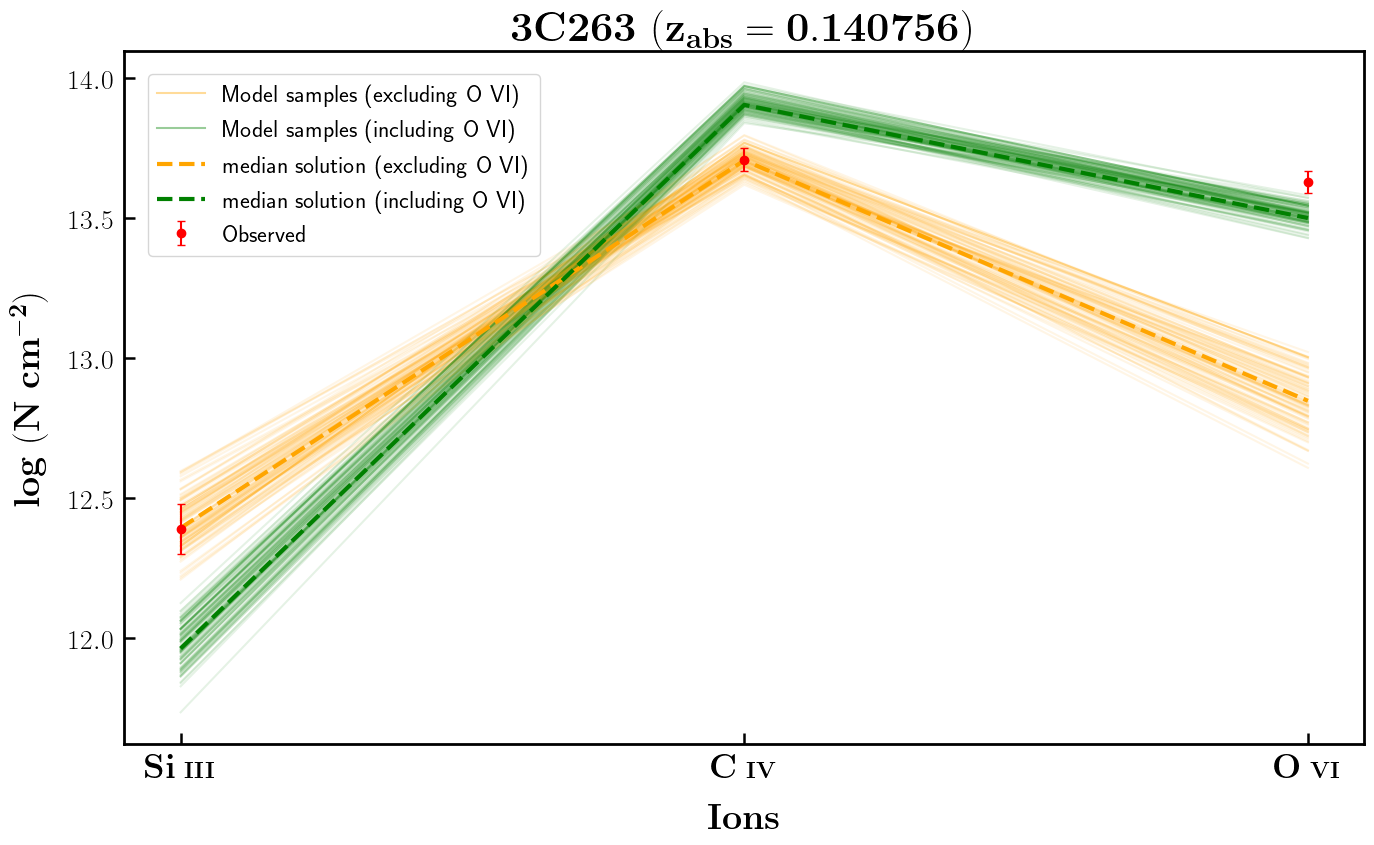
\includegraphics[width=0.85\linewidth]{Ionisation-Modelling-Plots/3c263-z=0.140756-compI_logZ=-1.png}
    \caption{N(\ion{H}{i})=13.49, log $Z_{ref}$=-1}
\end{figure}

\begin{figure}[!b]
    \centering
    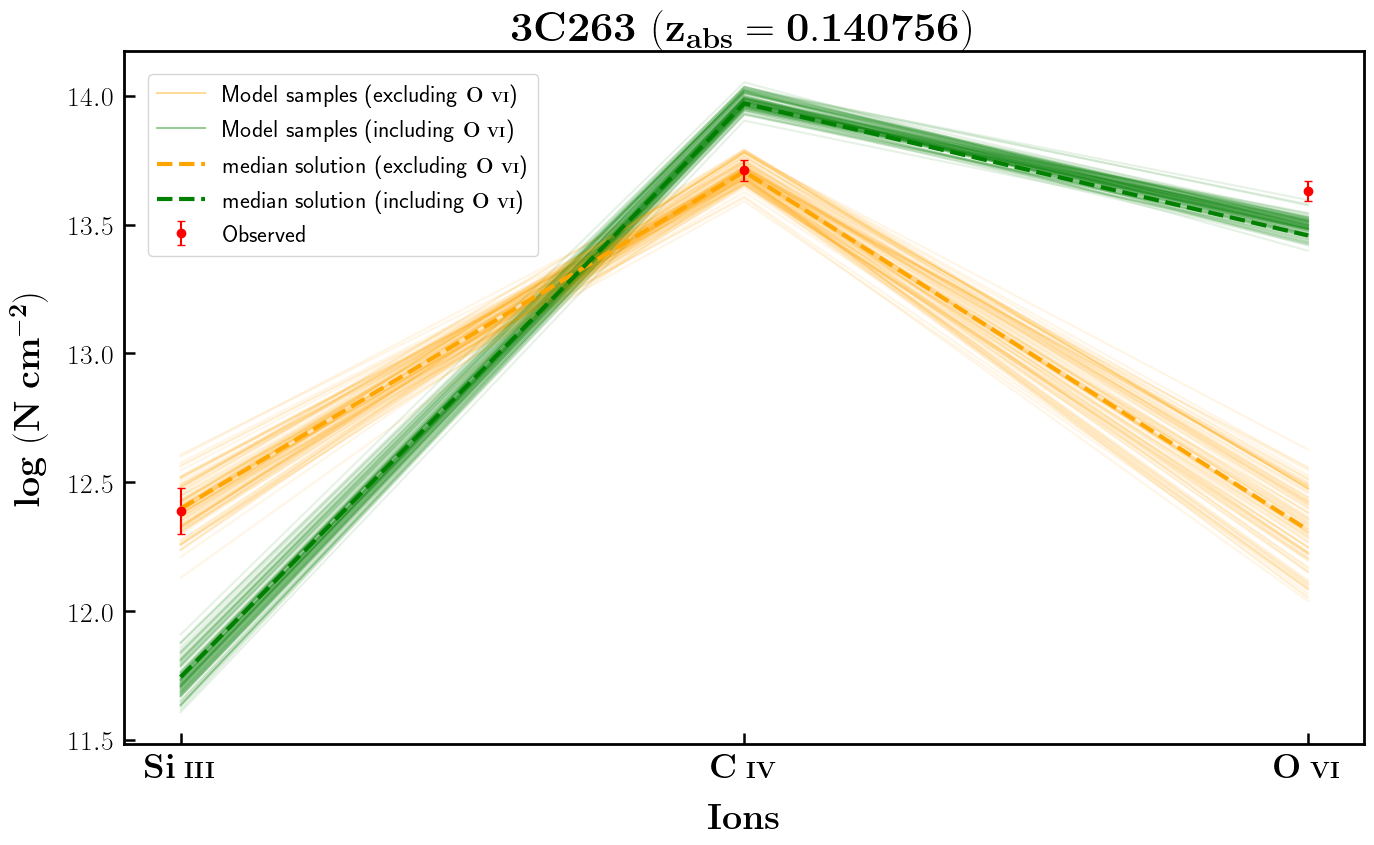
\includegraphics[width=0.85\linewidth]{Ionisation-Modelling-Plots/3c263-z=0.140756-compI_logZ=1.png}
    \caption{N(\ion{H}{i})=13.49, log $Z_{ref}$=1}
\end{figure}

\newpage

\textbf{Non-detections}

\begin{figure}[!h]
    \centering
    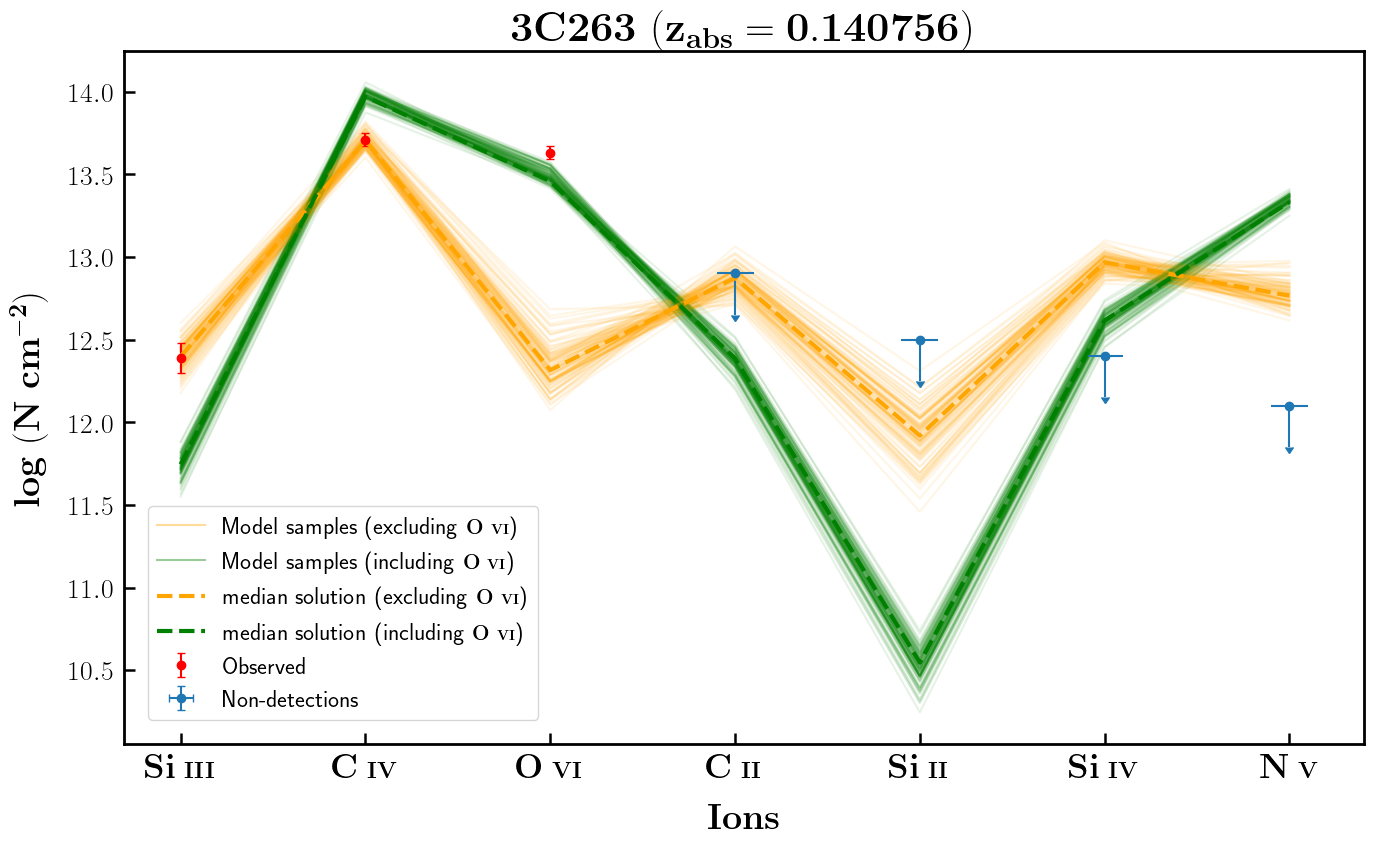
\includegraphics[width=1\linewidth]{Ionisation-Modelling-Plots/3c263-z=0.140756-compI_logZ=1_non_detection.png}
    \caption{N(\ion{H}{i})=13.49, log $Z_{ref}$=1}
\end{figure}



\newpage

\textbf{Comments}
\\
\begin{itemize}
    \item All 3 ions couldn't be explained together
    \item \ion{O}{vi} is underproduced when excluded
    \item Reference metallicity was initially used as logZ=-1, resulted in metallicity to be around 1, so later modelled with reference metallicity of logZ=1. 
    \item Ionisation : CI
    \item BLA : +ve
\end{itemize}




\newpage


\begin{landscape}

    \begin{figure}
    \centering
    \vspace{-20mm}
    \hspace*{-35mm}
    \captionsetup{oneside,margin={0cm,35mm}}
    \includegraphics[width=1.25\linewidth]{System-Plots/PKS0637-752_z=0.161064_sys_plot.png}
    \end{figure}
    
\end{landscape}


\begin{center}
 
\begin{tabular}{cccc}
        \hline \hline \tabularnewline
        \head{Ion} & \head{v (km s\textsuperscript{$\mathbf{-1}$})} & \head{b (km s\textsuperscript{$\mathbf{-1}$})} & \head{log [N cm\textsuperscript{$\mathbf{-2}$}]} 
        \tabularnewline \tabularnewline \hline \tabularnewline 

        \ion{N}{v}   &    -42 $\pm$ 6    &    40 $\pm$ 9    &     13.37 $\pm$ 0.07 \\
        \ion{Si}{iii}   &    11 $\pm$ 4    &    30 $\pm$ 7    &     12.37 $\pm$ 0.06 \\
        \ion{O}{vi}   &    0 $\pm$ 3    &    48 $\pm$ 5    &     14.02 $\pm$ 0.03 \\
        \ion{H}{i}   &    -13 $\pm$ 2    &    162 $\pm$ 21    &     13.6 $\pm$ 0.06 \\
        \ion{H}{i}   &    -1 $\pm$ 1    &    45 $\pm$ 1    &     15.01 $\pm$ 0.02 \\
\tabularnewline \hline \hline \tabularnewline

\end{tabular}

\end{center}

N(\ion{H}{I})=13.60 \\

log $Z_{ref}$ = -1 \\

Excluding \ion{O}{vi} : $n_H$ = -4.05 $\pm$ 0.03 \hspace{10mm} $Z$ = 1.20 $\pm$ 0.05

Including \ion{O}{vi} : $n_H$ = -4.12 $\pm$ 0.01 \hspace{10mm} $Z$ = 1.30 $\pm$ 0.04
\\\\

log $Z_{ref}$ = 1 \\

Excluding \ion{O}{vi} : $n_H$ = -4.29 $\pm$ 0.02 \hspace{10mm} $Z$ = 1.64 $\pm$ 0.05

Including \ion{O}{vi} : $n_H$ = -4.42 $\pm$ 0.01 \hspace{10mm} $Z$ = 1.69 $\pm$ 0.04

\newpage

\begin{figure}[!h]
    \centering
    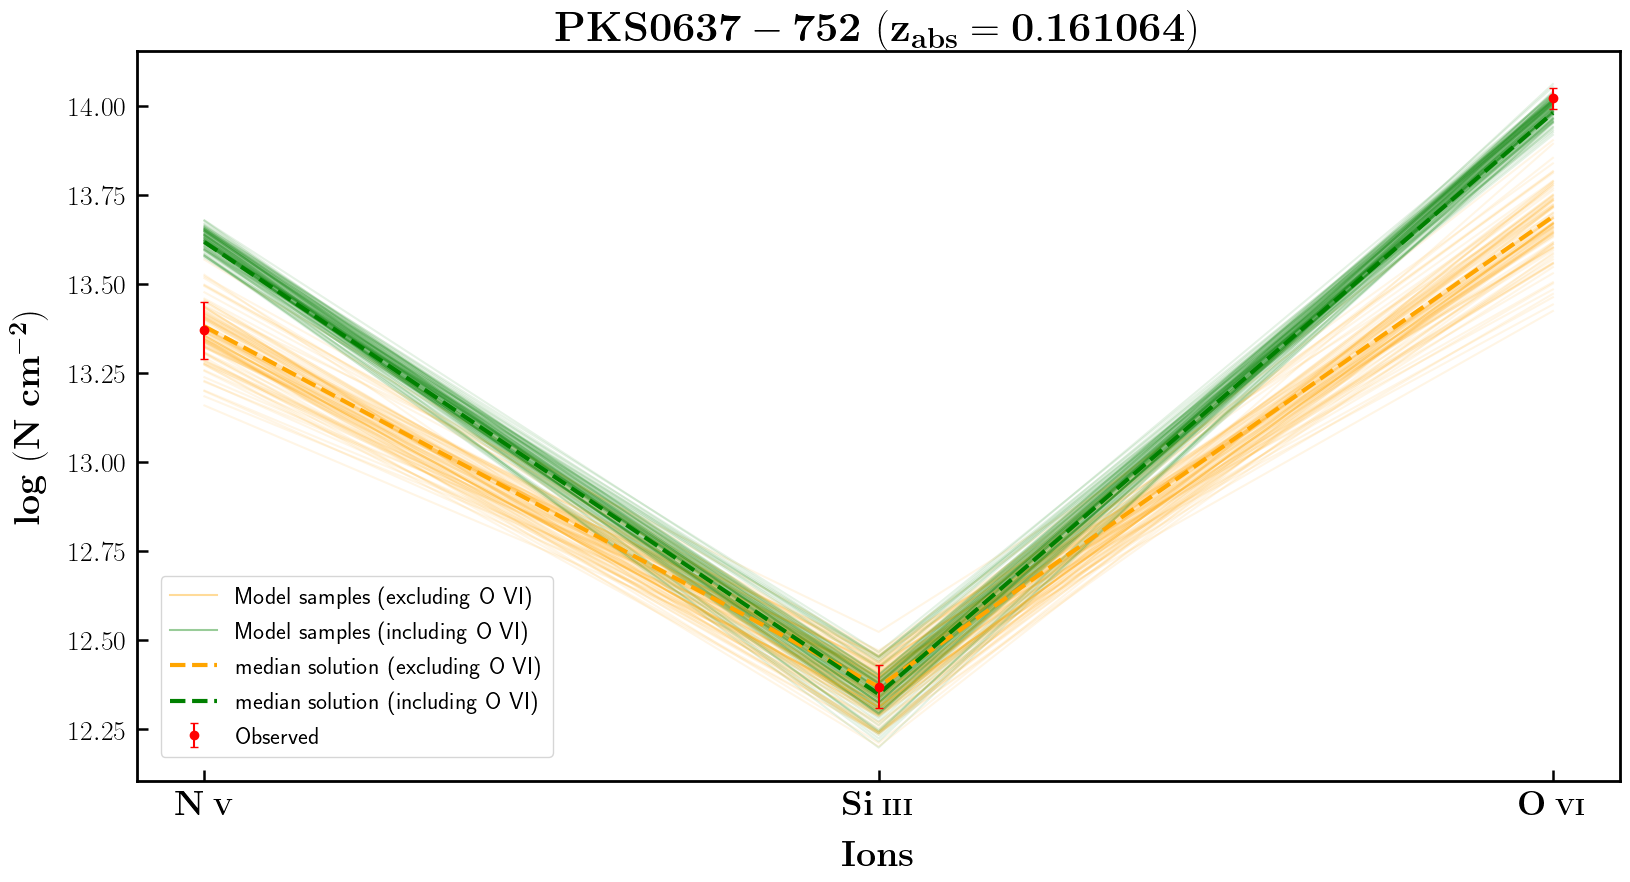
\includegraphics[width=0.85\linewidth]{Ionisation-Modelling-Plots/pks0637-z=0.161064-compI_logZ=-1.png}
    \caption{N(\ion{H}{i})=13.60, log $Z_{ref}$=-1}
\end{figure}

\begin{figure}[!b]
    \centering
    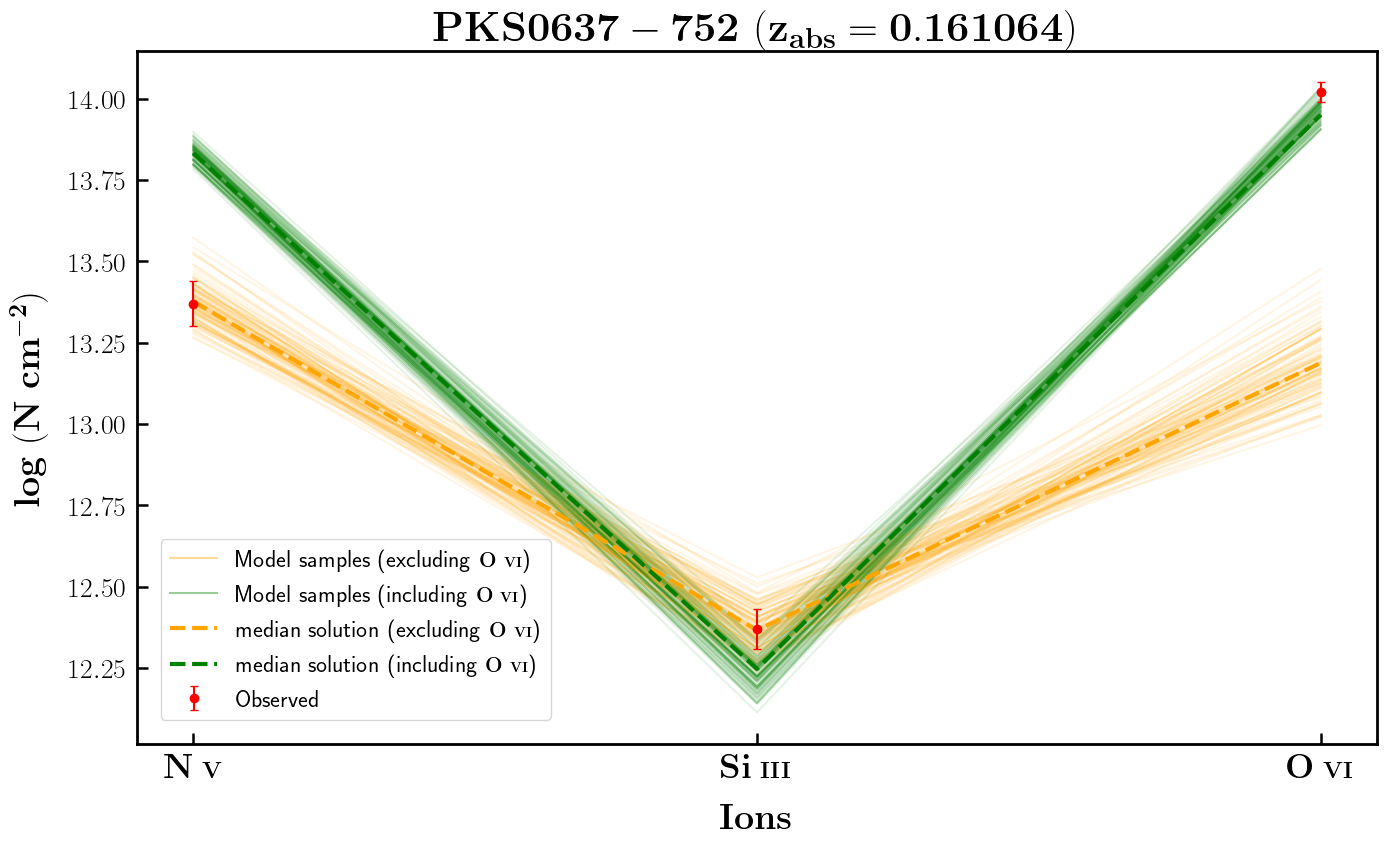
\includegraphics[width=0.85\linewidth]{Ionisation-Modelling-Plots/pks0637-z=0.161064-compI_logZ=1.png}
    \caption{N(\ion{H}{i})=13.60, log $Z_{ref}$=1}
\end{figure}

\newpage

\textbf{Non-detections}

\begin{figure}[!h]
    \centering
    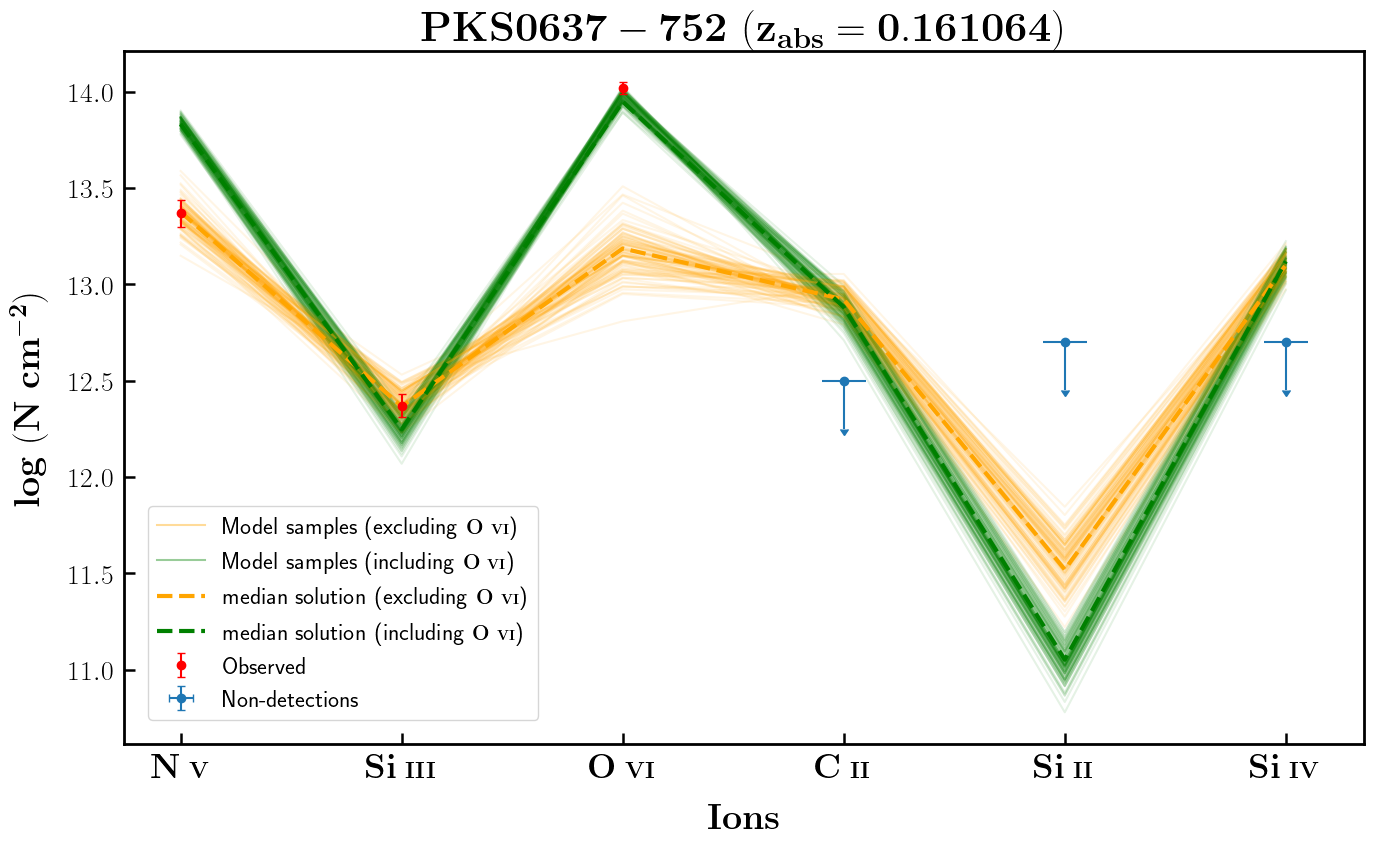
\includegraphics[width=1\linewidth]{Ionisation-Modelling-Plots/pks0637-z=0.161064-compI_logZ=1_non_detection.png}
    \caption{N(\ion{H}{i})=13.60, log $Z_{ref}$=1}
\end{figure}


\newpage

\textbf{Comments}
\\\\
\begin{itemize}
    \item large \emph{b} value
    \item All 3 ions couldn't be explained together
    \item When excluded \ion{O}{vi} is underproduced, but not significantly less, about an order of magnitude
    \item Modelled using both logZ=1 and logZ=-1 
    \item Ionisation : CI
    \item BLA : +ve
\end{itemize}


\newpage


\begin{landscape}

    \begin{figure}
    \centering
    \vspace{-20mm}
    \hspace*{-35mm}
    \captionsetup{oneside,margin={0cm,35mm}}
    \includegraphics[width=1.25\linewidth]{System-Plots/PKS0637-752_z=0.417539_sys_plot.png}
    \end{figure}
    
\end{landscape}


\begin{center}
    
    \begin{tabular}{cccc}
        \hline \hline \tabularnewline
        \head{Ion} & \head{v (km s\textsuperscript{$\mathbf{-1}$})} & \head{b (km s\textsuperscript{$\mathbf{-1}$})} & \head{log [N cm\textsuperscript{$\mathbf{-2}$}]} 
        \tabularnewline \tabularnewline \hline \tabularnewline 
    
        \ion{Si}{iii}   &    -5 $\pm$ 4    &    35 $\pm$ 7    &     12.74 $\pm$ 0.06 \\
        \ion{C}{iii}   &    -4 $\pm$ 1    &    24 $\pm$ 2    &     14.44 $\pm$ 0.15 \\
        \ion{O}{vi}   &    0 $\pm$ 1    &    42 $\pm$ 6    &     14.19 $\pm$ 0.05 \\
        \ion{H}{i}   &    -17 $\pm$ 1    &    30 $\pm$ 1    &     15.41 $\pm$ 0.03 \\
        \ion{H}{i}   &    20 $\pm$ 1    &    46 $\pm$ 4    &     14.61 $\pm$ 0.07 \\
        
        \tabularnewline \hline \hline \tabularnewline
    
    \end{tabular}
    
\end{center}
    
N(\ion{H}{I})=15.41 \\

Excluding \ion{O}{vi} : $n_H$ = -3.54 $\pm$ 0.11 \hspace{10mm} $Z$ = -0.49 $\pm$ 0.11

Including \ion{O}{vi} : $n_H$ = -3.74 $\pm$ 0.02 \hspace{10mm} $Z$ = -0.23 $\pm$ 0.04 \\

NOTE : MCMC walkers initialised near the solution for excluding \ion{O}{vi} case.
\\\\
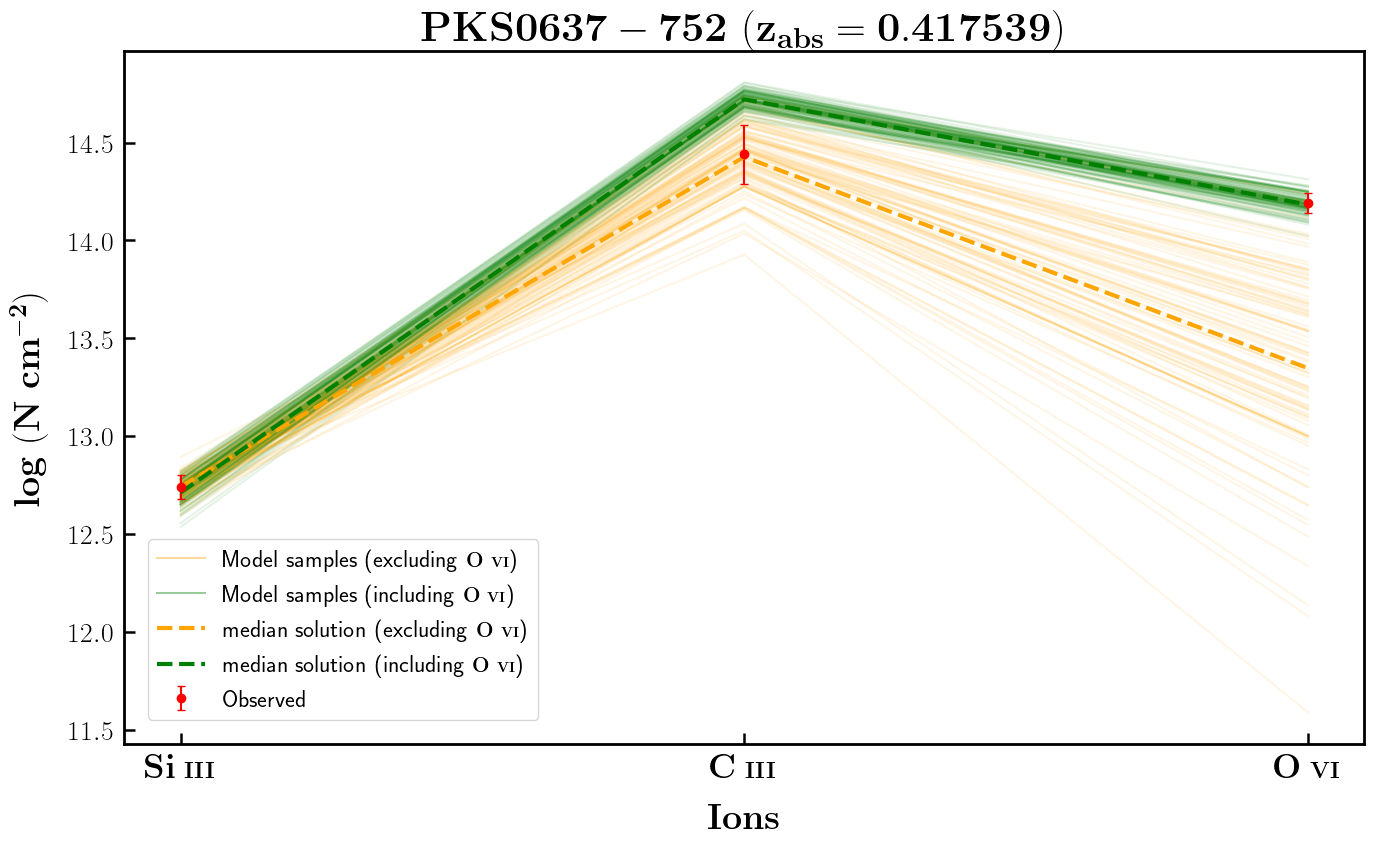
\includegraphics[width=1\linewidth]{Ionisation-Modelling-Plots/pks0637-z=0.417539-compI.png}


\newpage


\textbf{Non-detections}

\begin{figure}[!h]
    \centering
    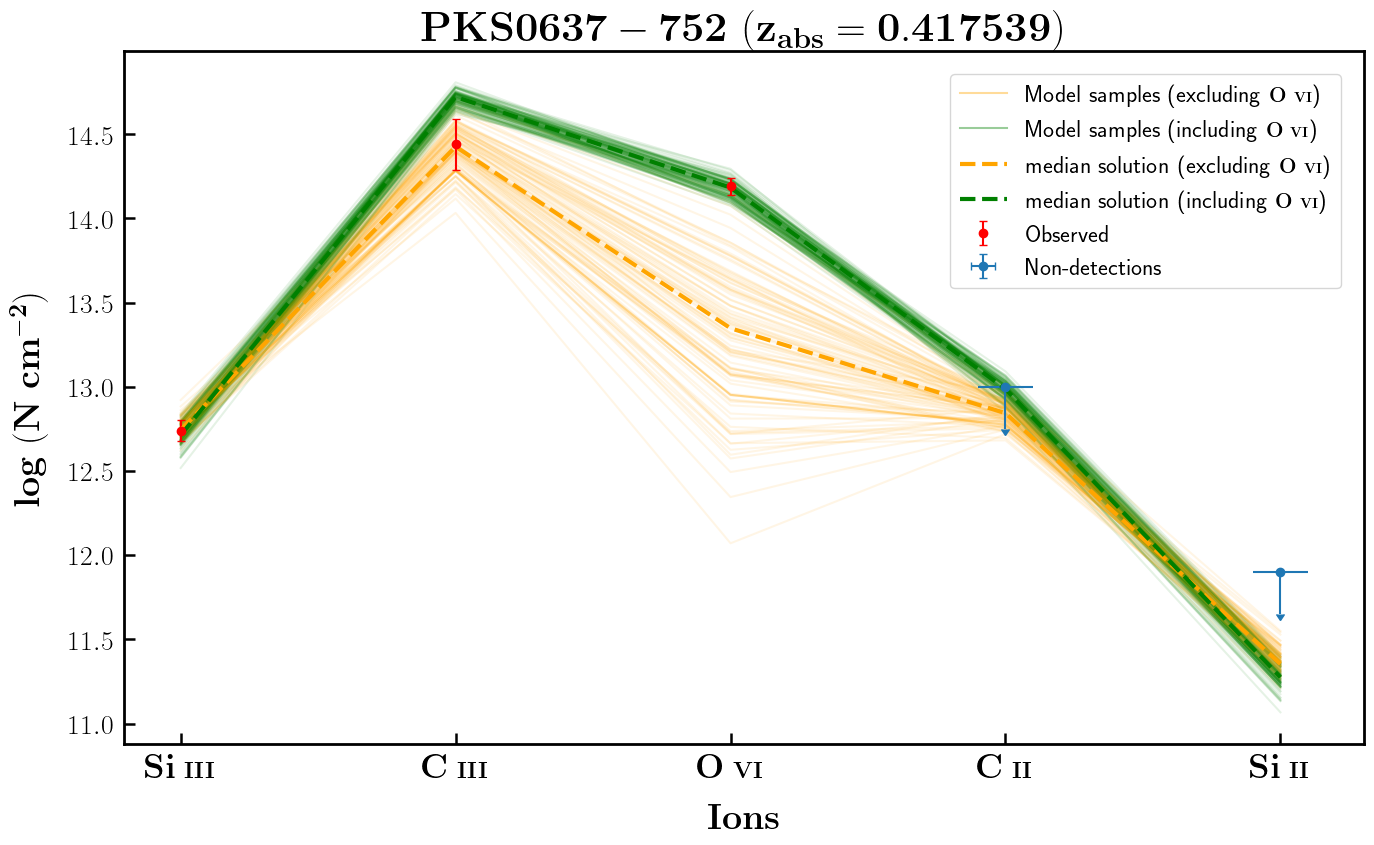
\includegraphics[width=1\linewidth]{Ionisation-Modelling-Plots/pks0637-z=0.417539-compI_logZ=-1_non_detection.png}
    \caption{N(\ion{H}{i})=15.41 , log $Z_{ref}$=-1}
\end{figure}



\newpage

\textbf{Comments}
\\\\
\begin{itemize}
    \item All 3 ions couldn't be explained together
    \item When excluded \ion{O}{vi} is underproduced
    \item Ionisation : CI
    \item BLA : +ve
\end{itemize}


\newpage


\begin{landscape}

    \begin{figure}
    \centering
    \vspace{-20mm}
    \hspace*{-35mm}
    \captionsetup{oneside,margin={0cm,35mm}}
    \includegraphics[width=1.25\linewidth]{System-Plots/PG1424+240_z=0.147104_sys_plot.png}
    \end{figure}
    
\end{landscape}


\begin{center}
    
    \begin{tabular}{cccc}
            \hline \hline \tabularnewline
            \head{Ion} & \head{v (km s\textsuperscript{$\mathbf{-1}$})} & \head{b (km s\textsuperscript{$\mathbf{-1}$})} & \head{log [N cm\textsuperscript{$\mathbf{-2}$}]} 
            \tabularnewline \tabularnewline \hline \tabularnewline 
    
            \ion{C}{iv}   &    -81 $\pm$ 2    &    11 $\pm$ 4    &     13.58 $\pm$ 0.09 \\
            \ion{C}{iv}   &    -18 $\pm$ 2    &    20 $\pm$ 3    &     14.06 $\pm$ 0.05 \\ \tabularnewline
            \ion{Si}{iii}   &    -78 $\pm$ 2    &    15 $\pm$ 3    &     12.58 $\pm$ 0.05 \\
            \ion{Si}{iii}   &    -9 $\pm$ 1    &    16 $\pm$ 2    &     12.87 $\pm$ 0.03 \\ \tabularnewline
            \ion{Si}{iv}   &    -82 $\pm$ 4    &    13 $\pm$ 7    &     12.69 $\pm$ 0.1 \\
            \ion{Si}{iv}   &    -11 $\pm$ 2    &    11 $\pm$ 5    &     12.88 $\pm$ 0.07 \\ \tabularnewline
            \ion{O}{vi}   &    -56 $\pm$ 9    &    39 $\pm$ 13    &     13.77 $\pm$ 0.11 \\
            \ion{O}{vi}   &    4 $\pm$ 4    &    16 $\pm$ 6    &     13.73 $\pm$ 0.11 \\ \tabularnewline
            \ion{H}{i}   &    -454 $\pm$ 3    &    27 $\pm$ 5    &     13.16 $\pm$ 0.05 \\
            \ion{H}{i}   &    -87 $\pm$ 3    &    23 $\pm$ 2    &     14.88 $\pm$ 0.05 \\
            \ion{H}{i}   &    0 $\pm$ 3    &    29 $\pm$ 2    &     15.44 $\pm$ 0.14 \\
            \ion{H}{i}   &    216 $\pm$ 2    &    40 $\pm$ 3    &     13.49 $\pm$ 0.02 \\
            \tabularnewline \hline \hline \tabularnewline
    
    \end{tabular}

\end{center}

N(\ion{H}{I})=15.44 \\

Excluding \ion{O}{vi} : $n_H$ = -3.81 $\pm$ 0.03 \hspace{10mm} $Z$ = -0.46 $\pm$ 0.03

Including \ion{O}{vi} : $n_H$ = -3.88 $\pm$ 0.02 \hspace{10mm} $Z$ = -0.42 $\pm$ 0.02
\\\\

N(\ion{H}{I})=14.88 \\

Excluding \ion{O}{vi} : $n_H$ = -3.74 $\pm$ 0.05 \hspace{10mm} $Z$ = -0.22 $\pm$ 0.04

Including \ion{O}{vi} : $n_H$ = -3.96 $\pm$ 0.03 \hspace{10mm} $Z$ = -0.07 $\pm$ 0.04
\\\\

\newpage

\begin{figure}[!h]
    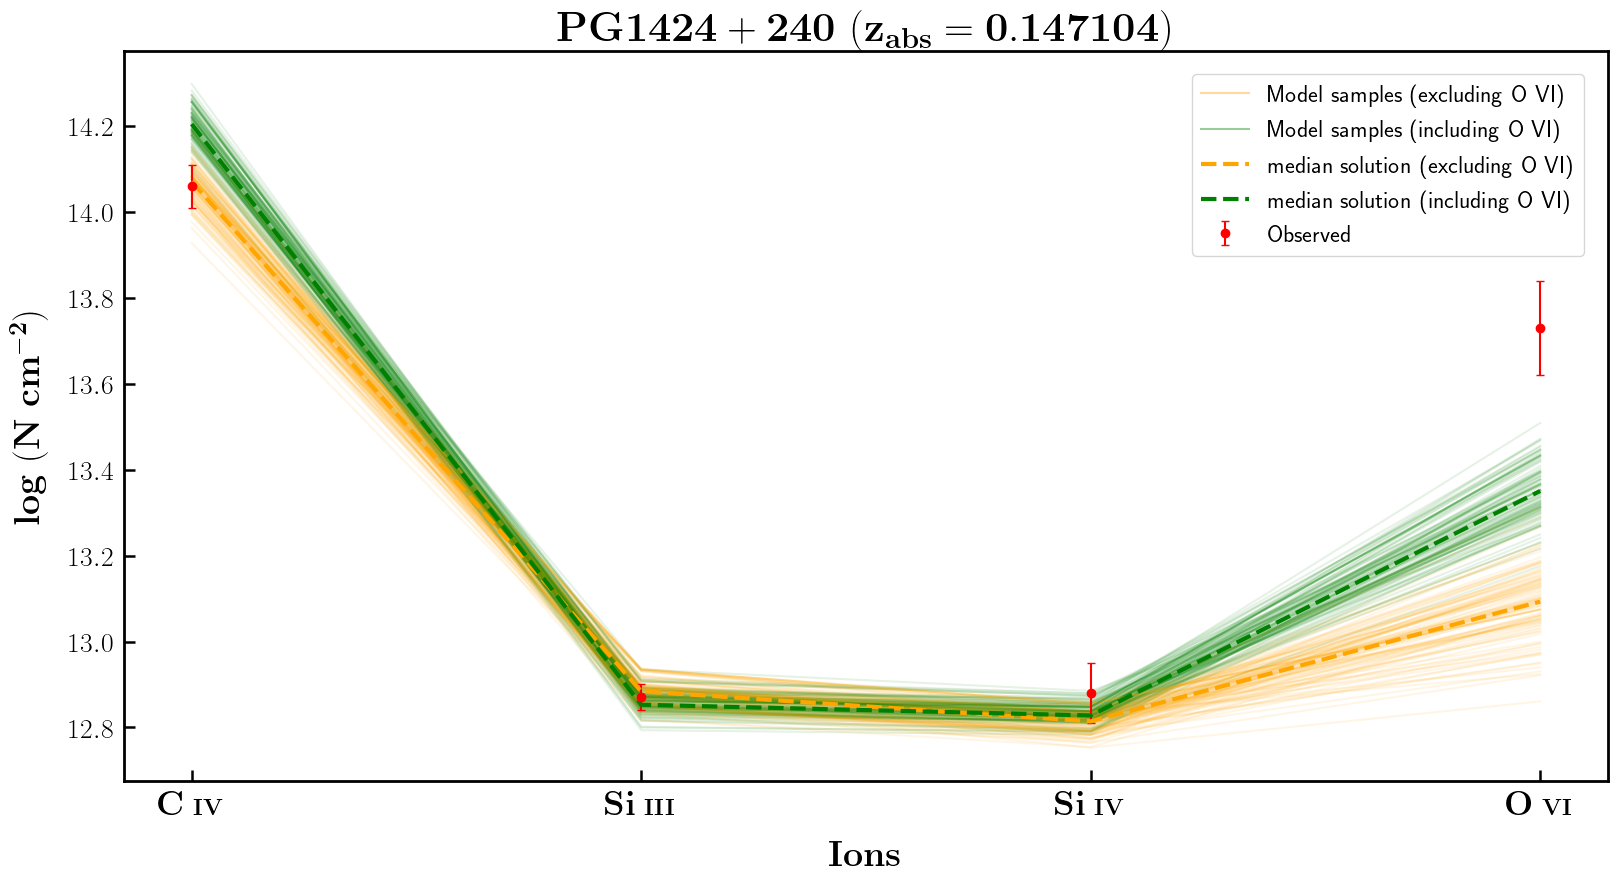
\includegraphics[width=0.8\linewidth]{Ionisation-Modelling-Plots/pg1424-z=0.147104-compIII.png}
    \caption{N(\ion{H}{i})=15.44}
\end{figure}

\begin{figure}[!b]
    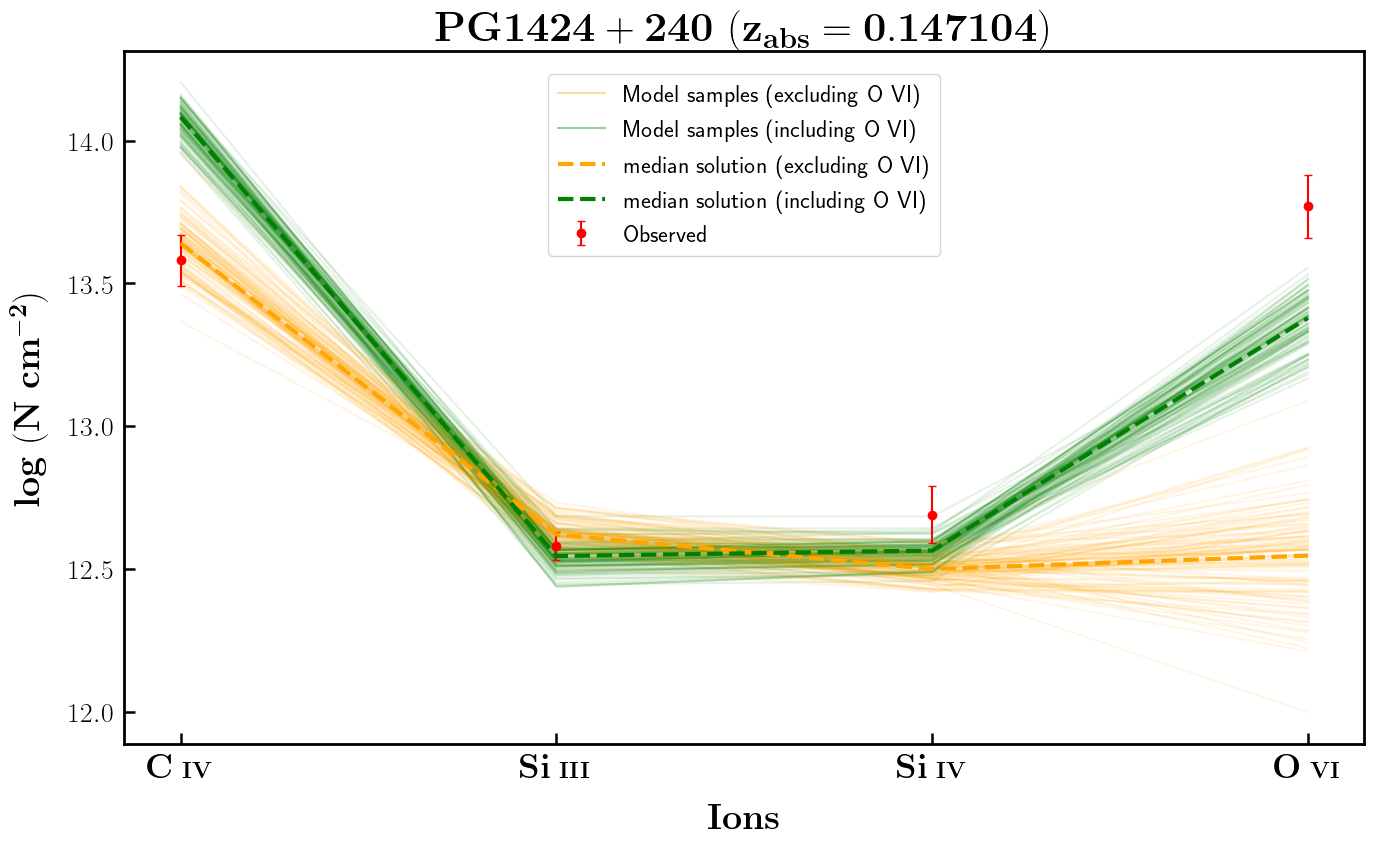
\includegraphics[width=0.8\linewidth]{Ionisation-Modelling-Plots/pg1424-z=0.147104-compII.png}
    \caption{N(\ion{H}{i})=14.88}
\end{figure}

\newpage

\textbf{Non-detections}

\begin{figure}[!h]
    \centering
    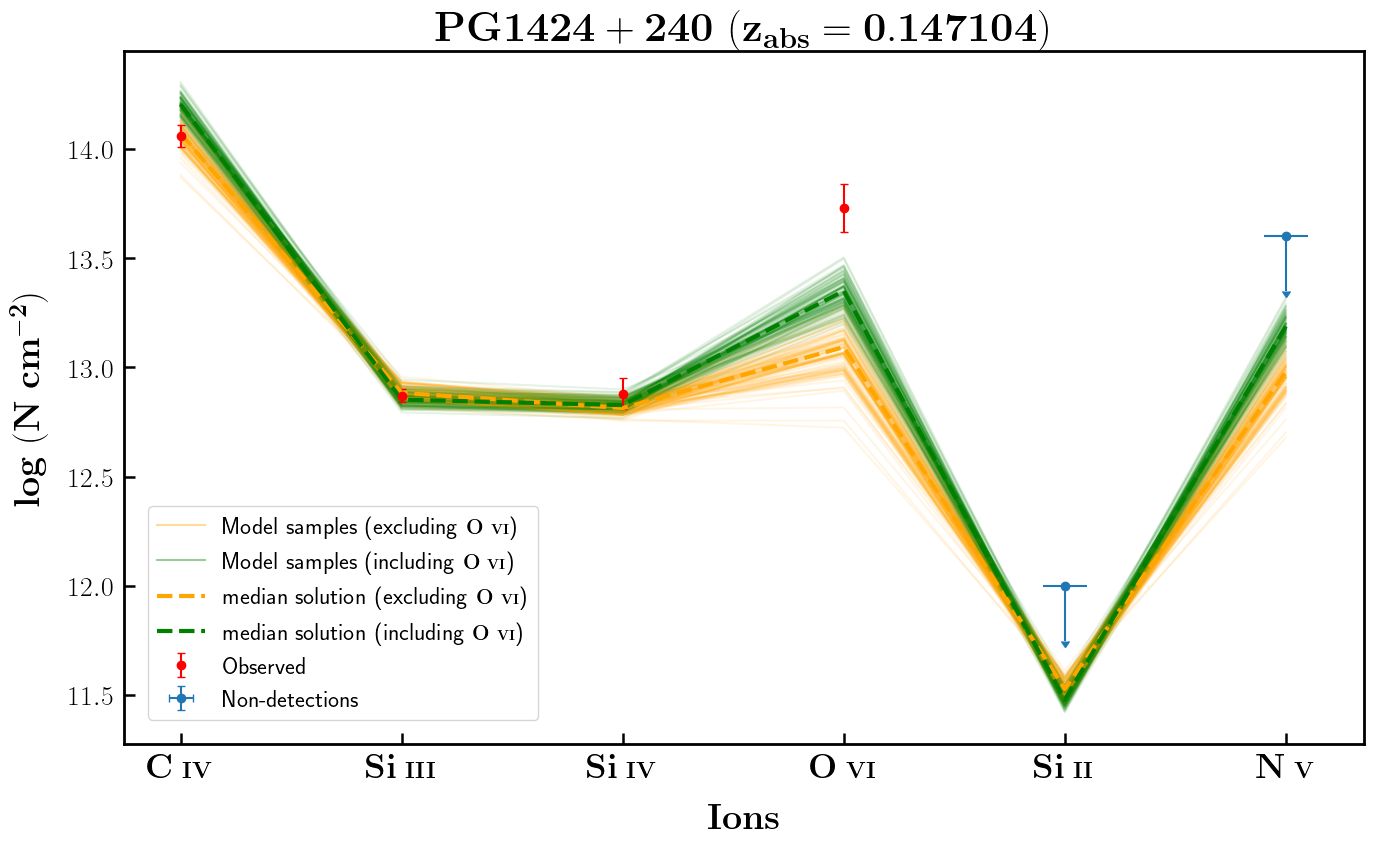
\includegraphics[width=0.85\linewidth]{Ionisation-Modelling-Plots/pg1424-z=0.147104-compIII_logZ=-1_non_detection.png}
    \caption{N(\ion{H}{i})= 15.44, log $Z_{ref}$=-1}
\end{figure}

\begin{figure}[!h]
    \centering
    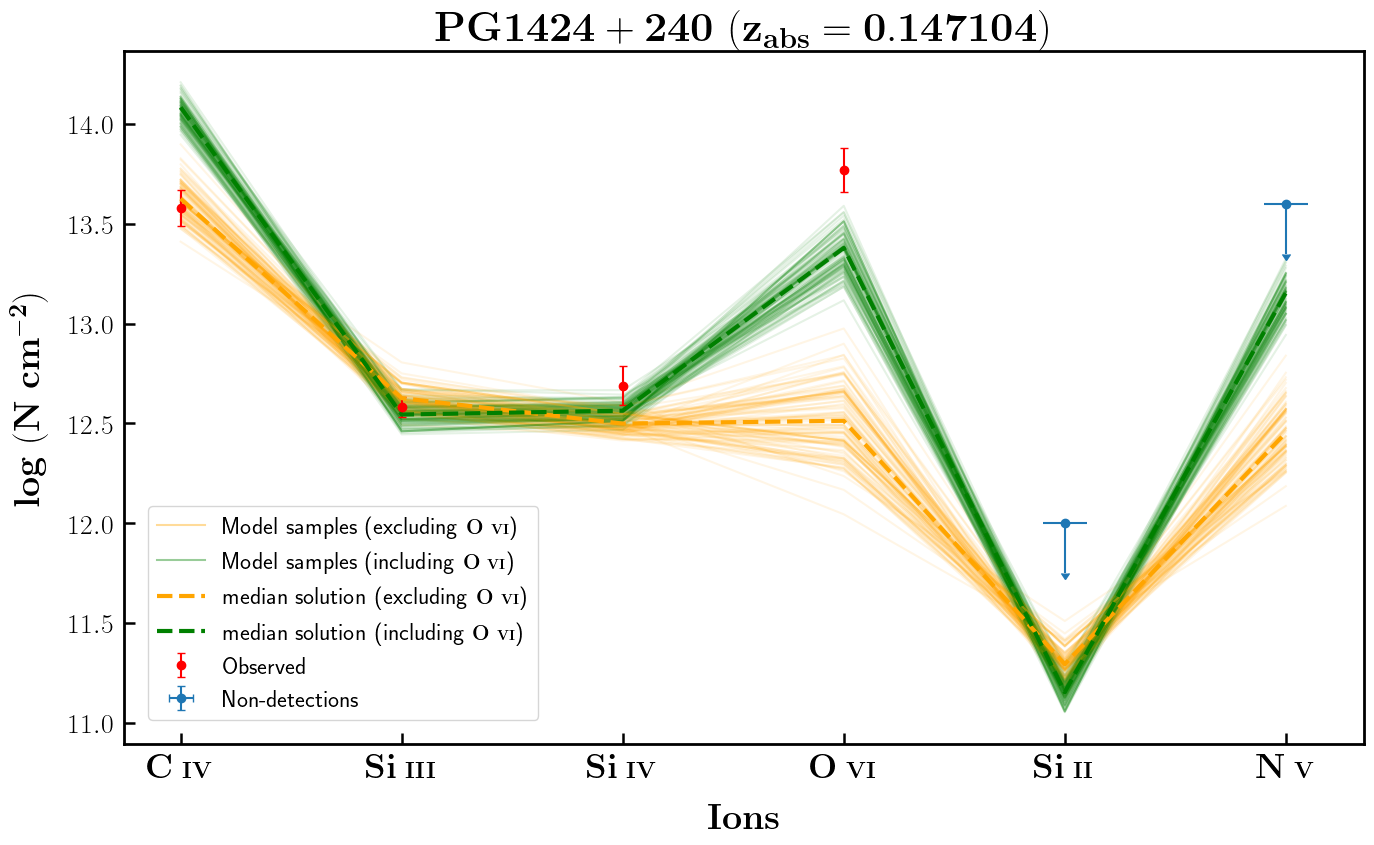
\includegraphics[width=0.85\linewidth]{Ionisation-Modelling-Plots/pg1424-z=0.147104-compII_logZ=-1_non_detection.png}
    \caption{N(\ion{H}{i})=14.88 , log $Z_{ref}$=-1}
\end{figure}



\newpage

\textbf{Comments}
\\\\
\begin{itemize}
    \item Smaller \emph{b} values 23 and 29 km/s
    \item All 4 ions couldn't be explained together
    \item Ions excluding \ion{O}{vi} could be explained together for both the components
    \item Ionisation : CI
    \item BLA : tentative - small b value but collisionally ionised
\end{itemize}


\newpage


\begin{landscape}

    \begin{figure}
    \centering
    \vspace{-20mm}
    \hspace*{-35mm}
    \captionsetup{oneside,margin={0cm,35mm}}
    \includegraphics[width=1.25\linewidth]{System-Plots/PG0003+158_z=0.386089_sys_plot.png}
    \end{figure}
    
\end{landscape}


\begin{center}
    
    \begin{tabular}{cccc}
        \hline \hline \tabularnewline
        \head{Ion} & \head{v (km s\textsuperscript{$\mathbf{-1}$})} & \head{b (km s\textsuperscript{$\mathbf{-1}$})} & \head{log [N cm\textsuperscript{$\mathbf{-2}$}]} 
        \tabularnewline \tabularnewline \hline \tabularnewline 
    
        \ion{O}{iii}   &    -18 $\pm$ 2    &    9 $\pm$ 5    &     13.93 $\pm$ 0.08 \\
        \ion{C}{iii}   &    -11 $\pm$ 1    &    13 $\pm$ 2    &     13.35 $\pm$ 0.05 \\
        \ion{N}{v}   &    -7 $\pm$ 1    &    33 $\pm$ 11    &     13.49 $\pm$ 0.11 \\
        \ion{O}{vi}   &    0 $\pm$ 2    &    25 $\pm$ 3    &     13.87 $\pm$ 0.04 \\
        \ion{O}{vi}   &    54 $\pm$ 3    &    25 $\pm$ 4    &     13.71 $\pm$ 0.06 \\
        \ion{H}{i}   &    -10 $\pm$ 1    &    29 $\pm$ 0    &     14.81 $\pm$ 0.03 \\
        \ion{H}{i}   &    40 $\pm$ 9    &    40 $\pm$ 4    &     14.1 $\pm$ 0.05 \\

        \tabularnewline \hline \hline \tabularnewline
    
    \end{tabular}
    
\end{center}
    
N(\ion{H}{I})=14.81 \\

Excluding \ion{O}{vi} : $n_H$ = -4.12 $\pm$ 0.06 \hspace{10mm} $Z$ = -0.65 $\pm$ 0.04

Including \ion{O}{vi} : $n_H$ = -4.07 $\pm$ 0.02 \hspace{10mm} $Z$ = -0.68 $\pm$ 0.03
\\\\
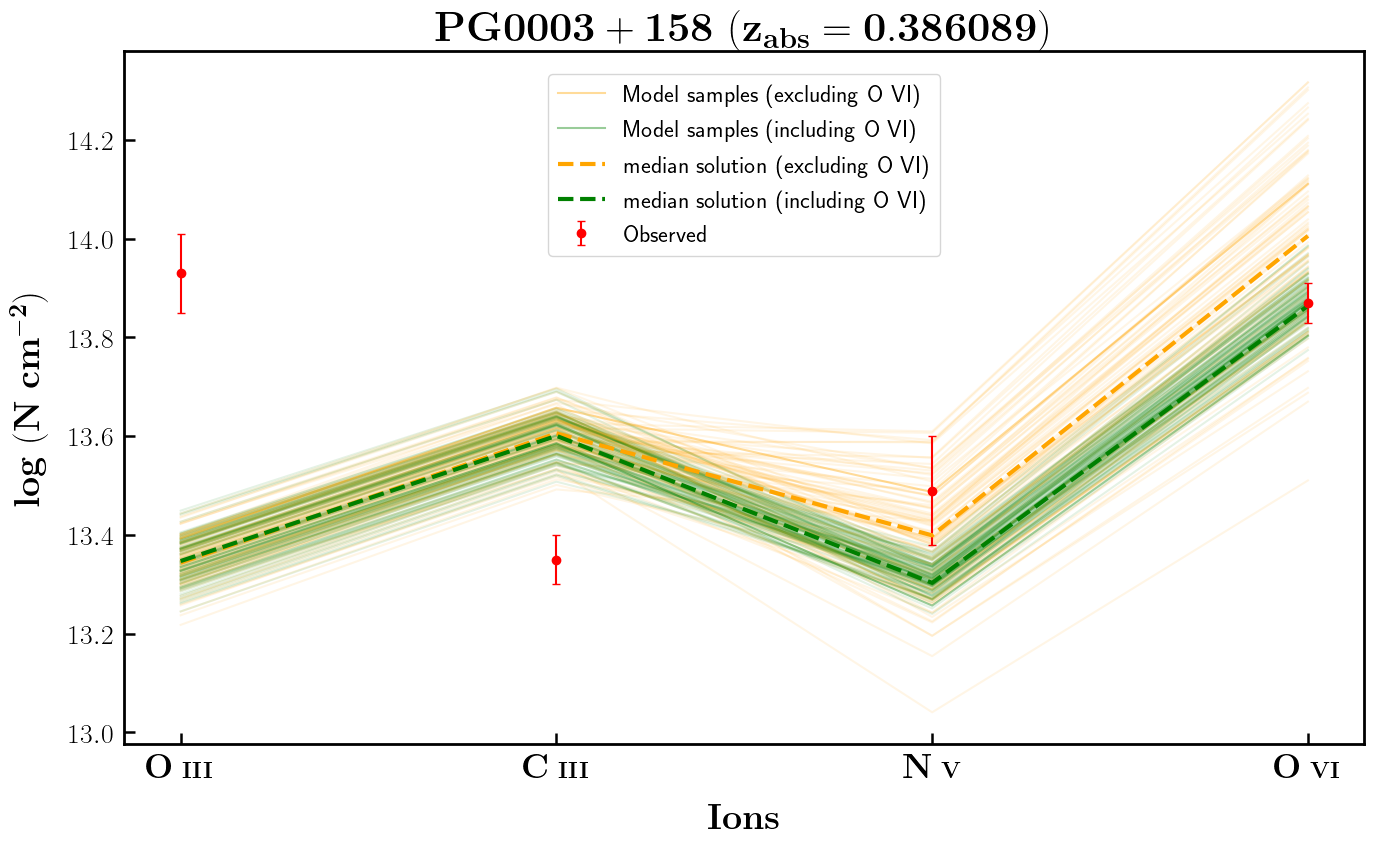
\includegraphics[width=1\linewidth]{Ionisation-Modelling-Plots/pg0003-z=0.386089-compI.png}


\newpage

\textbf{Non-detections}

\begin{figure}[!h]
    \centering
    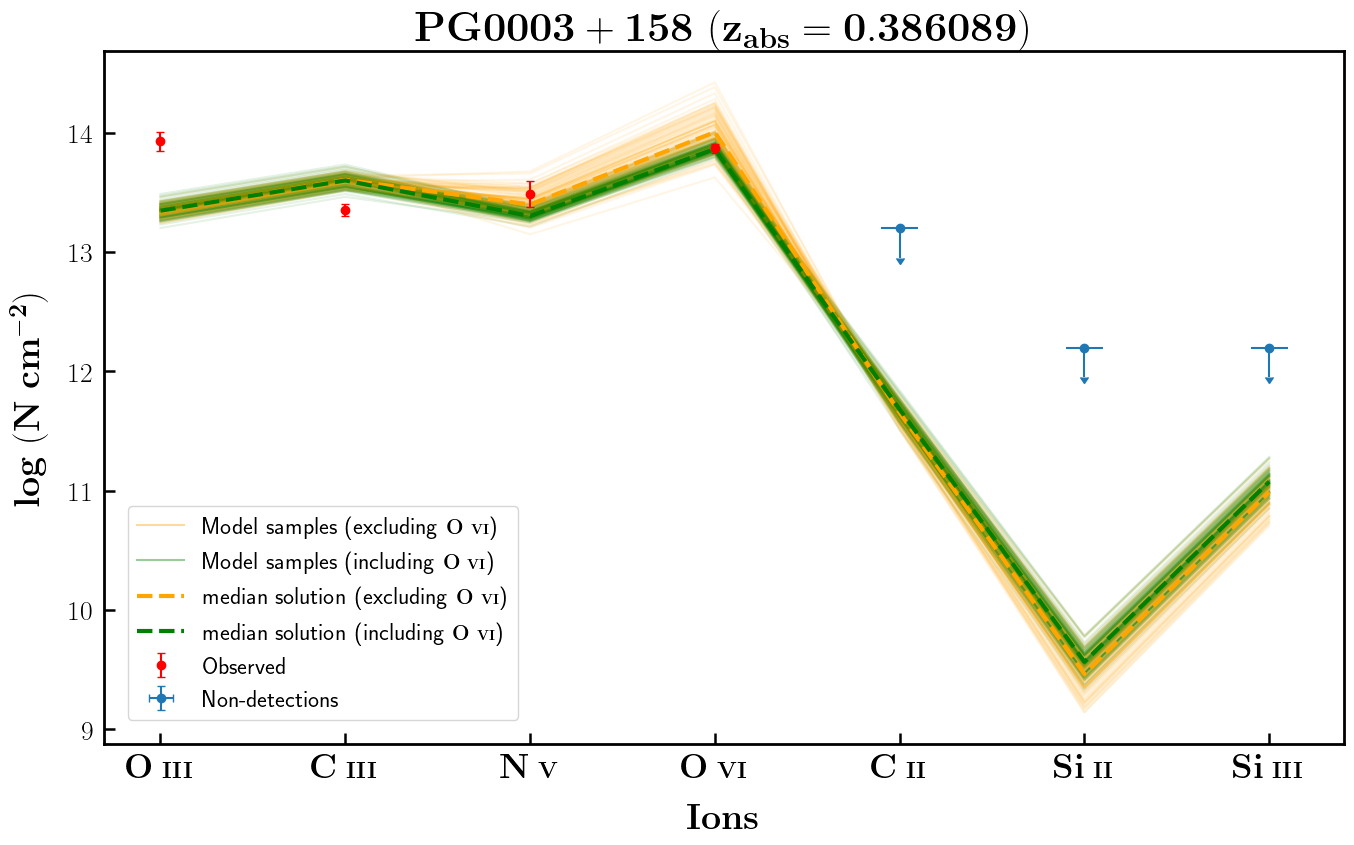
\includegraphics[width=1\linewidth]{Ionisation-Modelling-Plots/pg0003-z=0.386089-compI_logZ=-1_non_detection.png}
    \caption{N(\ion{H}{i})=14.81 , log $Z_{ref}$=-1}
\end{figure}



\newpage

\textbf{Comments}
\\\\
\begin{itemize}
    \item Not a good solution
    \item Ionisation : can't comment
    \item BLA : +ve
\end{itemize}



\newpage


\begin{landscape}

    \begin{figure}
    \centering
    \vspace{-20mm}
    \hspace*{-35mm}
    \captionsetup{oneside,margin={0cm,35mm}}
    \includegraphics[width=1.25\linewidth]{System-Plots/PG0003+158_z=0.421923_sys_plot.png}
    \end{figure}
    
\end{landscape}


\begin{center}
    
    \begin{tabular}{cccc}
        \hline \hline \tabularnewline
        \head{Ion} & \head{v (km s\textsuperscript{$\mathbf{-1}$})} & \head{b (km s\textsuperscript{$\mathbf{-1}$})} & \head{log [N cm\textsuperscript{$\mathbf{-2}$}]} 
        \tabularnewline \tabularnewline \hline \tabularnewline 
    
        \ion{C}{iii}   &    -9 $\pm$ 1    &    13 $\pm$ 1    &     13.35 $\pm$ 0.04 \\
        \ion{O}{iii}   &    -1 $\pm$ 2    &    7 $\pm$ 5    &     13.83 $\pm$ 0.13 \\
        \ion{O}{vi}   &    0 $\pm$ 1    &    27 $\pm$ 1    &     14.27 $\pm$ 0.02 \\
        \ion{H}{i}   &    -272 $\pm$ 6    &    66 $\pm$ 10    &     13.37 $\pm$ 0.05 \\
        \ion{H}{i}   &    -16 $\pm$ 1    &    64 $\pm$ 3    &     14.17 $\pm$ 0.04 \\
        \ion{H}{i}   &    -2 $\pm$ 1    &    26 $\pm$ 1    &     14.71 $\pm$ 0.02 \\
    
        \tabularnewline \hline \hline \tabularnewline
    
    \end{tabular}
    
\end{center}
    
N(\ion{H}{I})=14.17 \\

Excluding \ion{O}{vi} : $n_H$ = -2.66 $\pm$ 0.22 \hspace{10mm} $Z$ = 0.42 $\pm$ 0.23

Including \ion{O}{vi} : $n_H$ = -4.24 $\pm$ 0.02 \hspace{10mm} $Z$ = -0.09 $\pm$ 0.03 \\

NOTE : Convergence is not good for excluding \ion{O}{vi} case
\\\\
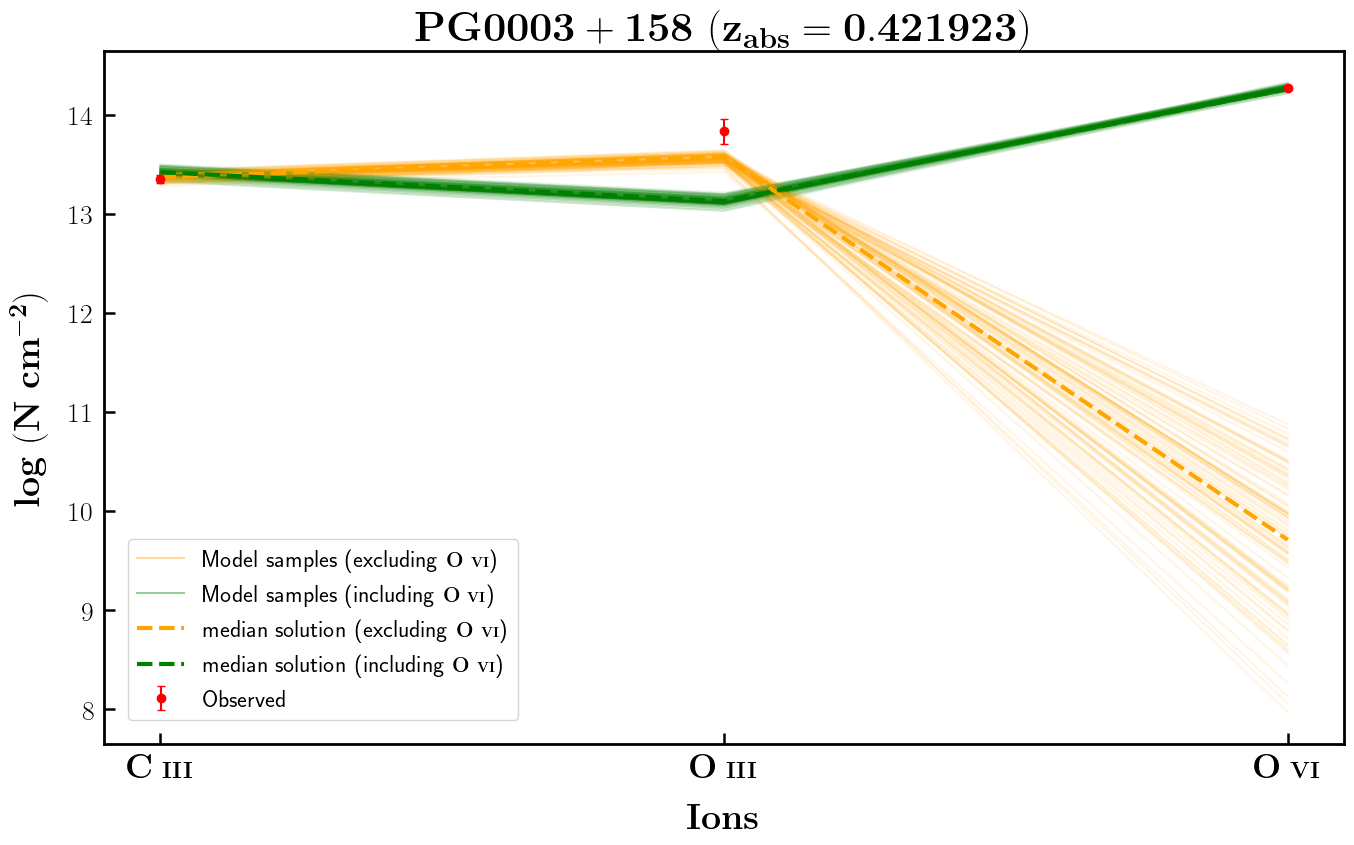
\includegraphics[width=1\linewidth]{Ionisation-Modelling-Plots/pg0003-z=0.421923-compII.png}
    

\newpage

\textbf{Non-detections}

\begin{figure}[!h]
    \centering
    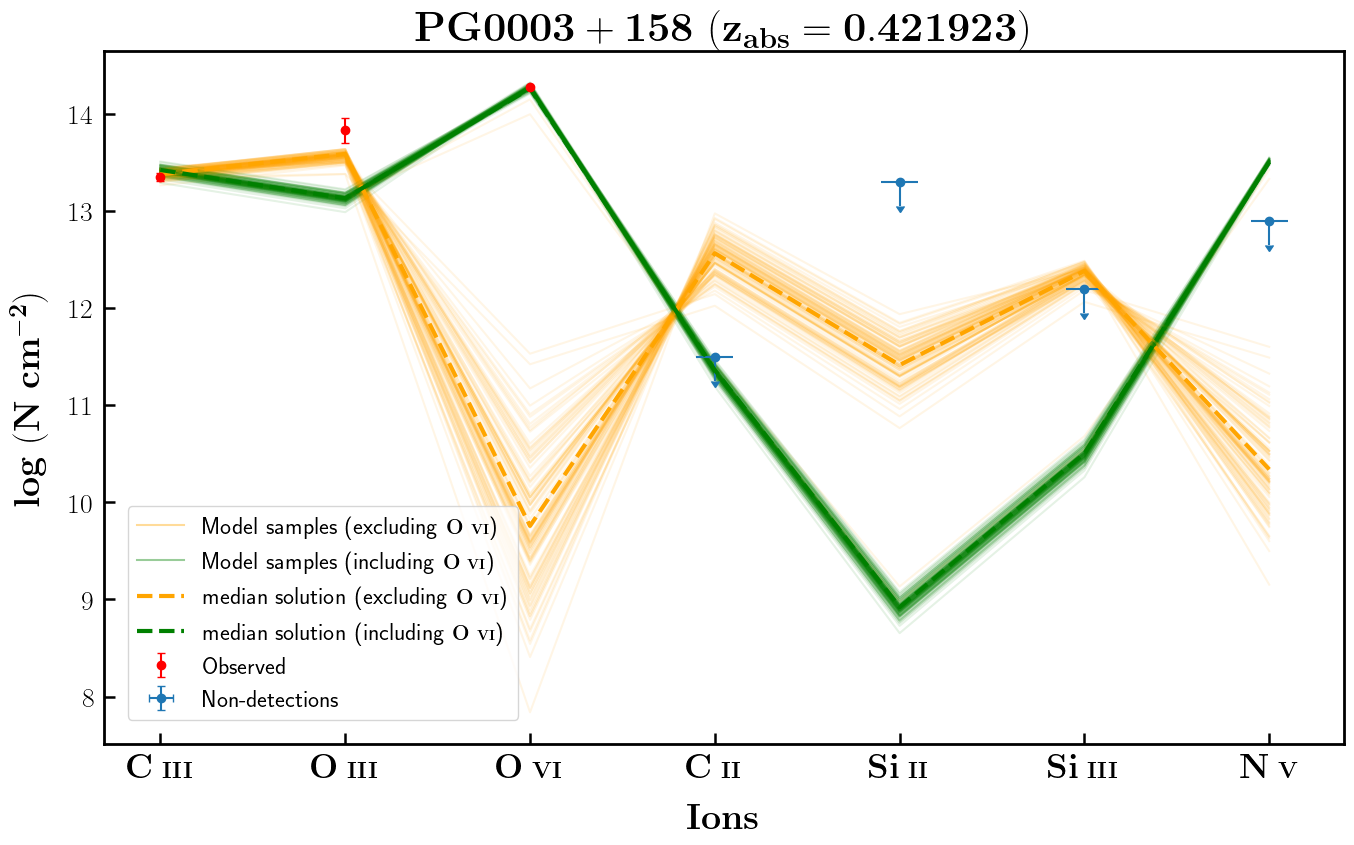
\includegraphics[width=1\linewidth]{Ionisation-Modelling-Plots/pg0003-z=0.421923-compII_logZ=-1_non_detection.png}
    \caption{N(\ion{H}{i})=14.17 , log $Z_{ref}$=-1}
\end{figure}


\newpage

\textbf{Comments}
\\\\
\begin{itemize}
    \item All 3 ions couldn't be explained together
    \item When excluded \ion{O}{vi} is heavily underproduced
    \item Convergence is not good for excluding \ion{O}{vi} case
    \item Ionisation : CI
    \item BLA : +ve
\end{itemize}



\newpage


\begin{landscape}

    \begin{figure}
    \centering
    \vspace{-20mm}
    \hspace*{-35mm}
    \captionsetup{oneside,margin={0cm,35mm}}
    \includegraphics[width=1.25\linewidth]{System-Plots/PG1216+069_z=0.282286_sys_plot.png}
    \end{figure}
    
\end{landscape}


\begin{center}
 
\begin{tabular}{cccc}
        \hline \hline \tabularnewline
        \head{Ion} & \head{v (km s\textsuperscript{$\mathbf{-1}$})} & \head{b (km s\textsuperscript{$\mathbf{-1}$})} & \head{log [N cm\textsuperscript{$\mathbf{-2}$}]} 
        \tabularnewline \tabularnewline \hline \tabularnewline 

        \ion{Si}{iii}   &    0 $\pm$ 1    &    14 $\pm$ 3    &     12.92 $\pm$ 0.05 \\
        \ion{C}{iii}   &    -51 $\pm$ 3    &    32 $\pm$ 5    &     13.33 $\pm$ 0.05 \\
        \ion{C}{iii}   &    5 $\pm$ 1    &    16 $\pm$ 2    &     13.76 $\pm$ 0.07 \\
        \ion{O}{vi}   &    -64 $\pm$ 6    &    58 $\pm$ 9    &     13.93 $\pm$ 0.05 \\
        \ion{O}{vi}   &    19 $\pm$ 2    &    12 $\pm$ 5    &     13.54 $\pm$ 0.09 \\
        \ion{H}{i}   &    -31 $\pm$ 1    &    52 $\pm$ 3    &     15.1 $\pm$ 0.05 \\
        \ion{H}{i}   &    7 $\pm$ 1    &    22 $\pm$ 1    &     16.4 $\pm$ 0.03 \\
        \ion{H}{i}   &    169 $\pm$ 22    &    53 $\pm$ 10    &     13.15 $\pm$ 0.18 \\

        \tabularnewline \hline \hline \tabularnewline

\end{tabular}
    
\end{center}
    
N(\ion{H}{I})=15.10 \\

Excluding \ion{O}{vi} : $n_H$ = -2.13 $\pm$ 0.15 \hspace{10mm} $Z$ = 0.65 $\pm$ 0.22

Including \ion{O}{vi} : $n_H$ = -3.86 $\pm$ 0.02 \hspace{10mm} $Z$ = -0.37 $\pm$ 0.03 \\

NOTE : Convergence is not much good for excluding \ion{O}{vi} case
\\\\

N(\ion{H}{I})=16.40 \\

Excluding \ion{O}{vi} : $n_H$ = -2.08 $\pm$ 0.43 \hspace{10mm} $Z$ = -0.37 $\pm$ 0.59

Including \ion{O}{vi} : $n_H$ = -3.68 $\pm$ 0.02 \hspace{10mm} $Z$ = -1.55 $\pm$ 0.04 \\

NOTE : Convergence is not much good for excluding \ion{O}{vi} case


\newpage


\begin{figure}[!h]
    \centering
    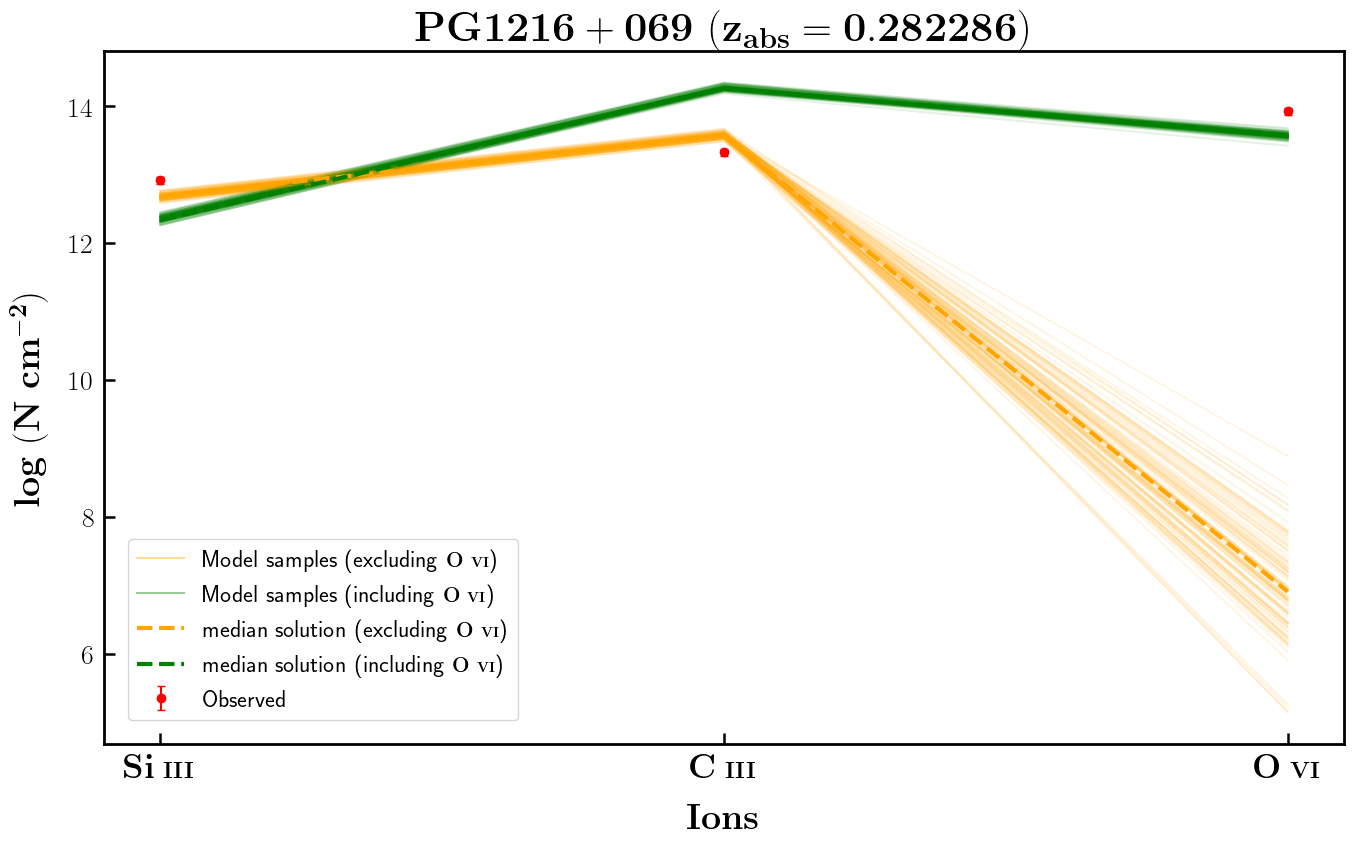
\includegraphics[width=0.85\linewidth]{Ionisation-Modelling-Plots/pg1216-z=0.282286-compI.png}
    \caption{N(\ion{H}{i})=15.10}
\end{figure}

\begin{figure}[!b]
    \centering
    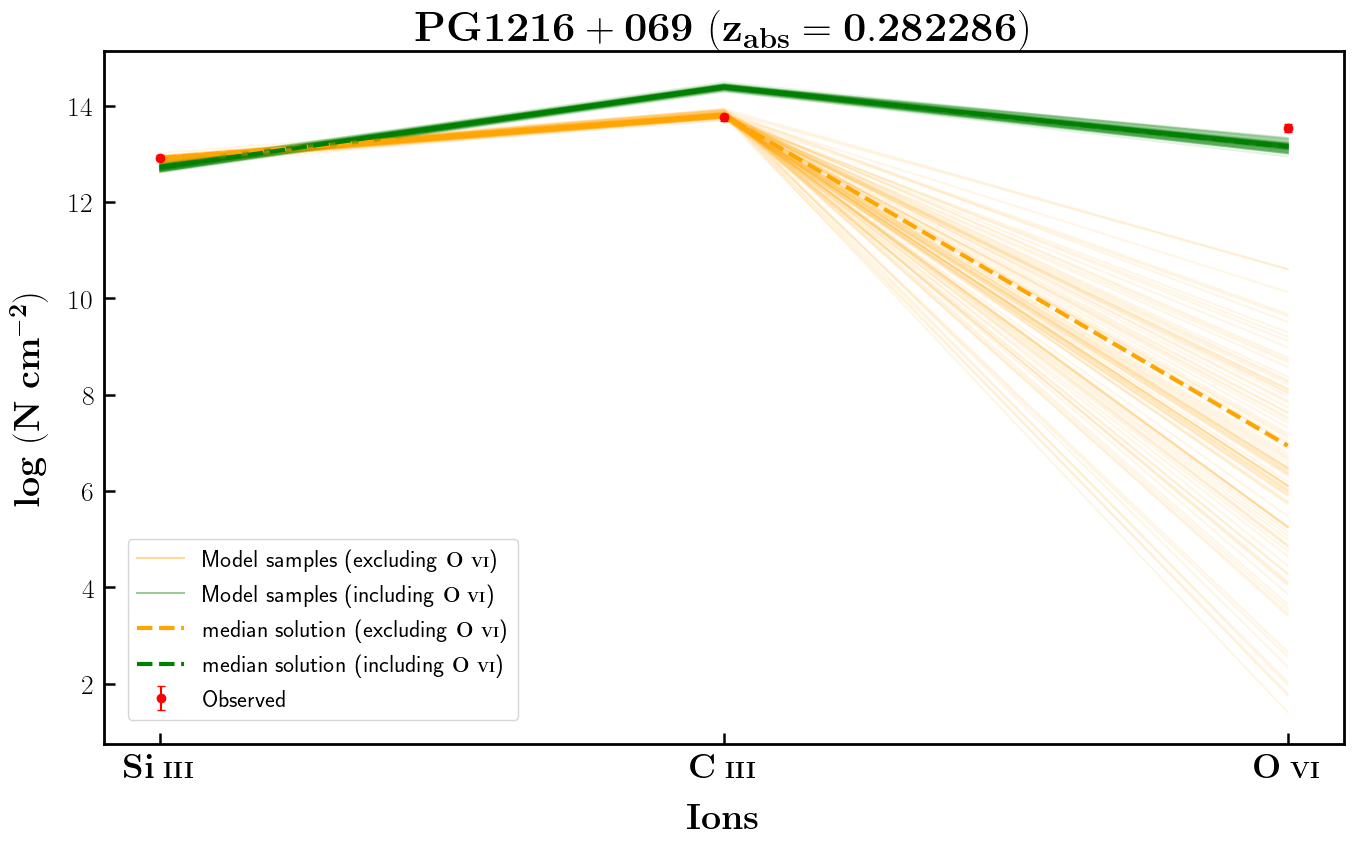
\includegraphics[width=0.85\linewidth]{Ionisation-Modelling-Plots/pg1216-z=0.282286-compII.png}
    \caption{N(\ion{H}{i})=16.40}
\end{figure}


\newpage

\textbf{Non-detections}

\begin{figure}[!h]
    \centering
    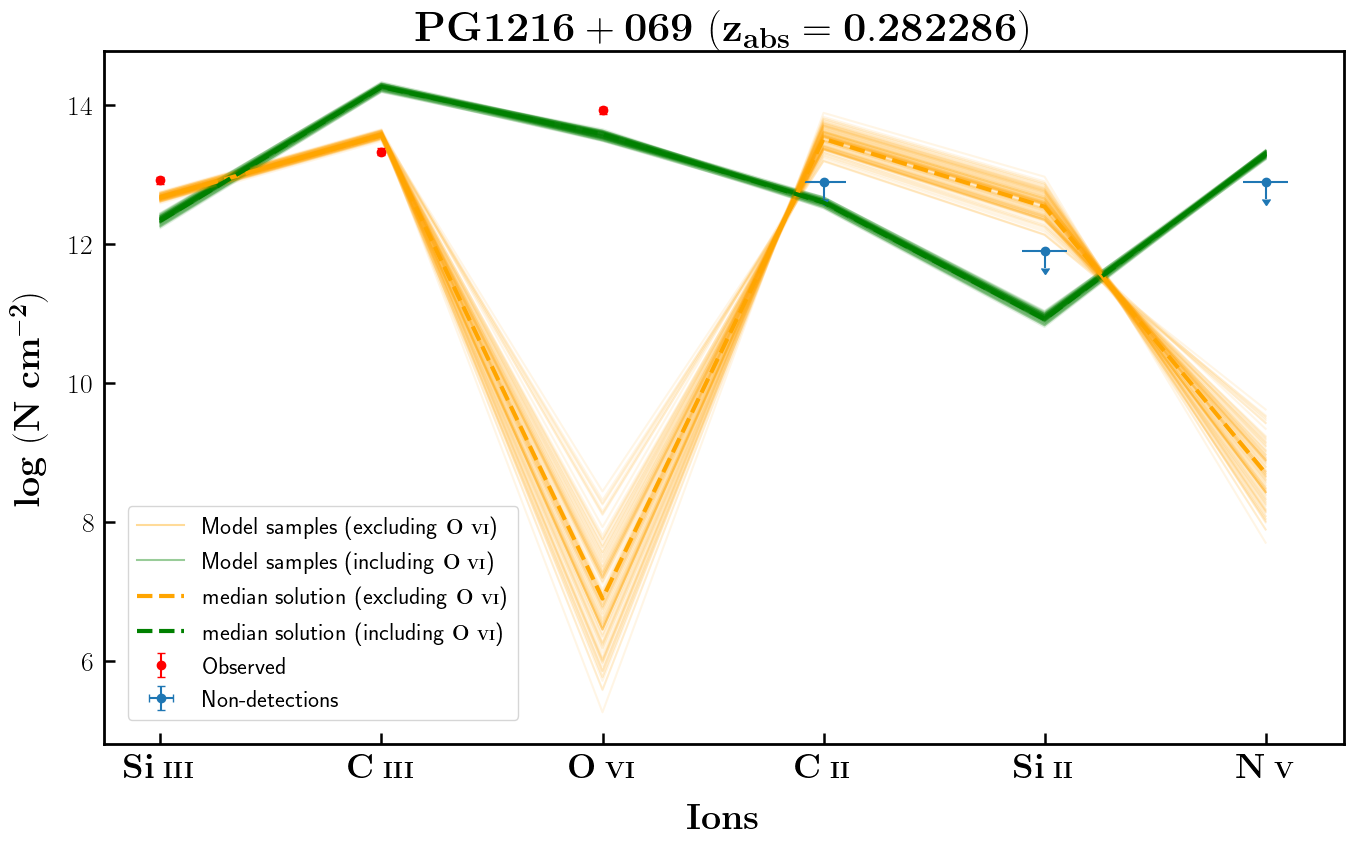
\includegraphics[width=0.85\linewidth]{Ionisation-Modelling-Plots/pg1216-z=0.282286-compI_logZ=-1_non_detection.png}
    \caption{N(\ion{H}{i})=15.10, log $Z_{ref}$=-1}
\end{figure}

\begin{figure}[!h]
    \centering
    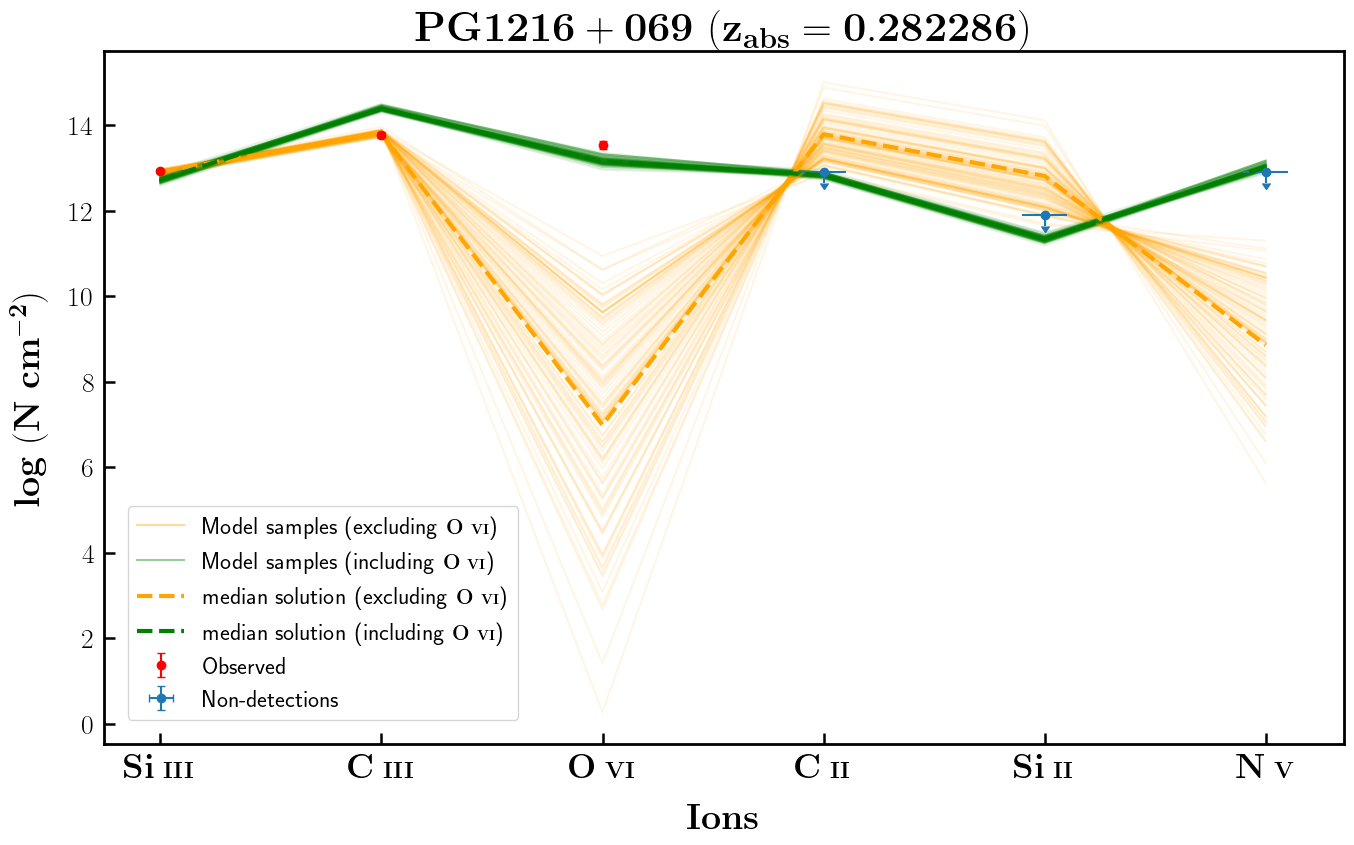
\includegraphics[width=0.85\linewidth]{Ionisation-Modelling-Plots/pg1216-z=0.282286-compII_logZ=-1_non_detection.png}
    \caption{N(\ion{H}{i})=16.40, log $Z_{ref}$=-1}
\end{figure}


\newpage

\textbf{Comments}
\\\\
\begin{itemize}
    \item Results similar for both the components
    \item All 3 ions couldn't be explained together
    \item When excluded \ion{O}{vi} is heavily underproduced
    \item Convergence is not much good for excluding \ion{O}{vi} case
    \item Ionisation : CI
    \item BLA : +ve
\end{itemize}


\newpage

\begin{landscape}

\begin{figure}
    \centering
    \vspace{-20mm}
    \hspace*{-35mm}
    \captionsetup{oneside,margin={0cm,35mm}}
    \includegraphics[width=1.25\linewidth]{System-Plots/SDSSJ135712.61+170444_z=0.097869_sys_plot.png}
\end{figure}

\end{landscape}


\begin{center} 

\begin{tabular}{cccc} 

    \hline \hline \tabularnewline 
    \head{Ion} & \head{v (km s\textsuperscript{$\mathbf{-1}$})} & \head{b (km s\textsuperscript{$\mathbf{-1}$})} & \head{log [N cm\textsuperscript{$\mathbf{-2}$}]}
    \tabularnewline \tabularnewline \hline \tabularnewline 
 
    \ion{Si}{iii}   &    -62 $\pm$ 2    &    17 $\pm$ 3    &     12.94 $\pm$ 0.05 \\
    \ion{Si}{iii}   &    4 $\pm$ 1    &    13 $\pm$ 10    &     14.67 $\pm$ 2.87 \\
    \ion{C}{iv}   &    -74 $\pm$ 6    &    33 $\pm$ 1    &     13.82 $\pm$ 0.09 \\
    \ion{C}{iv}   &    -7 $\pm$ 8    &    32 $\pm$ 12    &     13.63 $\pm$ 0.12 \\
    \ion{Si}{iv}   &    -66 $\pm$ 4    &    18 $\pm$ 6    &     13.02 $\pm$ 0.08 \\
    \ion{Si}{iv}   &    0 $\pm$ 4    &    29 $\pm$ 5    &     13.3 $\pm$ 0.05 \\
    \ion{C}{ii}   &    -79 $\pm$ 8    &    19 $\pm$ 14    &     13.17 $\pm$ 0.16 \\
    \ion{C}{ii}   &    -1 $\pm$ 2    &    22 $\pm$ 3    &     13.92 $\pm$ 0.04 \\
    \ion{O}{vi}   &    -96 $\pm$ 10    &    43 $\pm$ 16    &     14.3 $\pm$ 0.11 \\
    \ion{H}{i}   &    -536 $\pm$ 3    &    29 $\pm$ 5    &     13.36 $\pm$ 0.05 \\
    \ion{H}{i}   &    -66 $\pm$ 0    &    29 $\pm$ 8    &     16.49 $\pm$ 0.12 \\
    \ion{H}{i}   &    0 $\pm$ 0    &    46 $\pm$ 4    &     15.01 $\pm$ 0.16 \\
    \ion{H}{i}   &    424 $\pm$ 3    &    34 $\pm$ 4    &     13.52 $\pm$ 0.04 \\

    \tabularnewline \hline \hline \tabularnewline 

\end{tabular}

\end{center}


N(\ion{H}{I})=16.49  (log $Z_{ref}$=-1) \\

Excluding \ion{O}{vi} : $n_H$ = -3.76 $\pm$ 0.05 \hspace{10mm} $Z$ = -1.49 $\pm$ 0.04

Including \ion{O}{vi} : $n_H$ = -4.06 $\pm$ 0.02 \hspace{10mm} $Z$ = -1.32 $\pm$ 0.04
\\\\

N(\ion{H}{I})=15.01 \\

log $Z_{ref}$=-1 

Excluding \ion{O}{vi} : $n_H$ = -3.25 $\pm$ 0.04 \hspace{10mm} $Z$ = 0.93 $\pm$ 0.04

Including \ion{O}{vi} : $n_H$ = -3.84 $\pm$ 0.03 \hspace{10mm} $Z$ = 0.75 $\pm$ 0.03  \\

log $Z_{ref}$=1 

Excluding \ion{O}{vi} : $n_H$ = -3.7 $\pm$ 0.03 \hspace{10mm} $Z$ = 1.35 $\pm$ 0.04

Including \ion{O}{vi} : $n_H$ = -4.30 $\pm$ 0.03 \hspace{10mm} $Z$ = 1.00 $\pm$ 0.03 \\

NOTE : Using \ion{O}{vi} column density from other component to compare.

\newpage


\begin{figure}[!h]
    \centering
    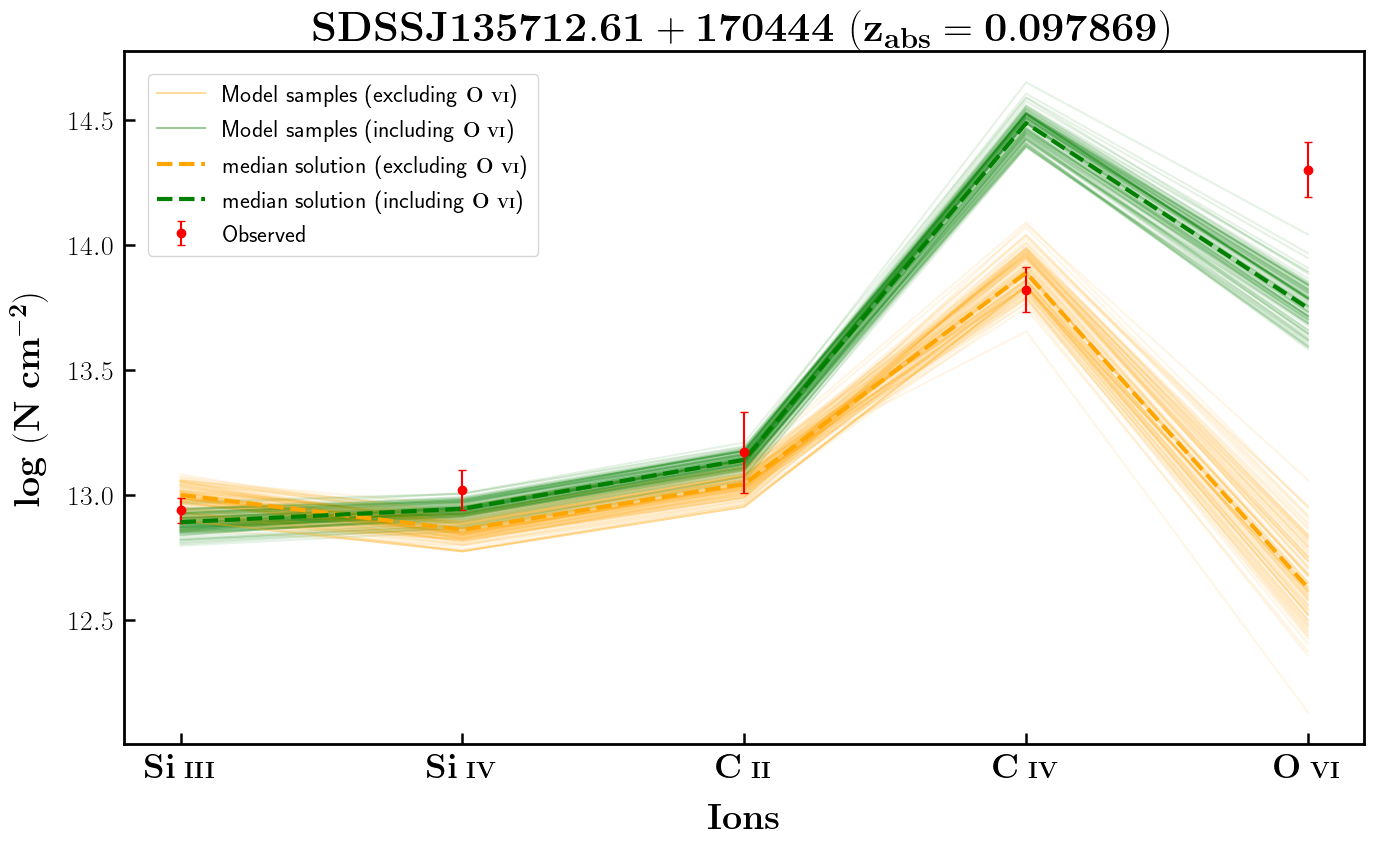
\includegraphics[width=0.85\linewidth]{Ionisation-Modelling-Plots/s135712-z=0.097869-compII.png}
    \caption{N(\ion{H}{i})=16.49, log $Z_{ref}$=-1}
\end{figure}

\begin{figure}[!b]
    \centering
    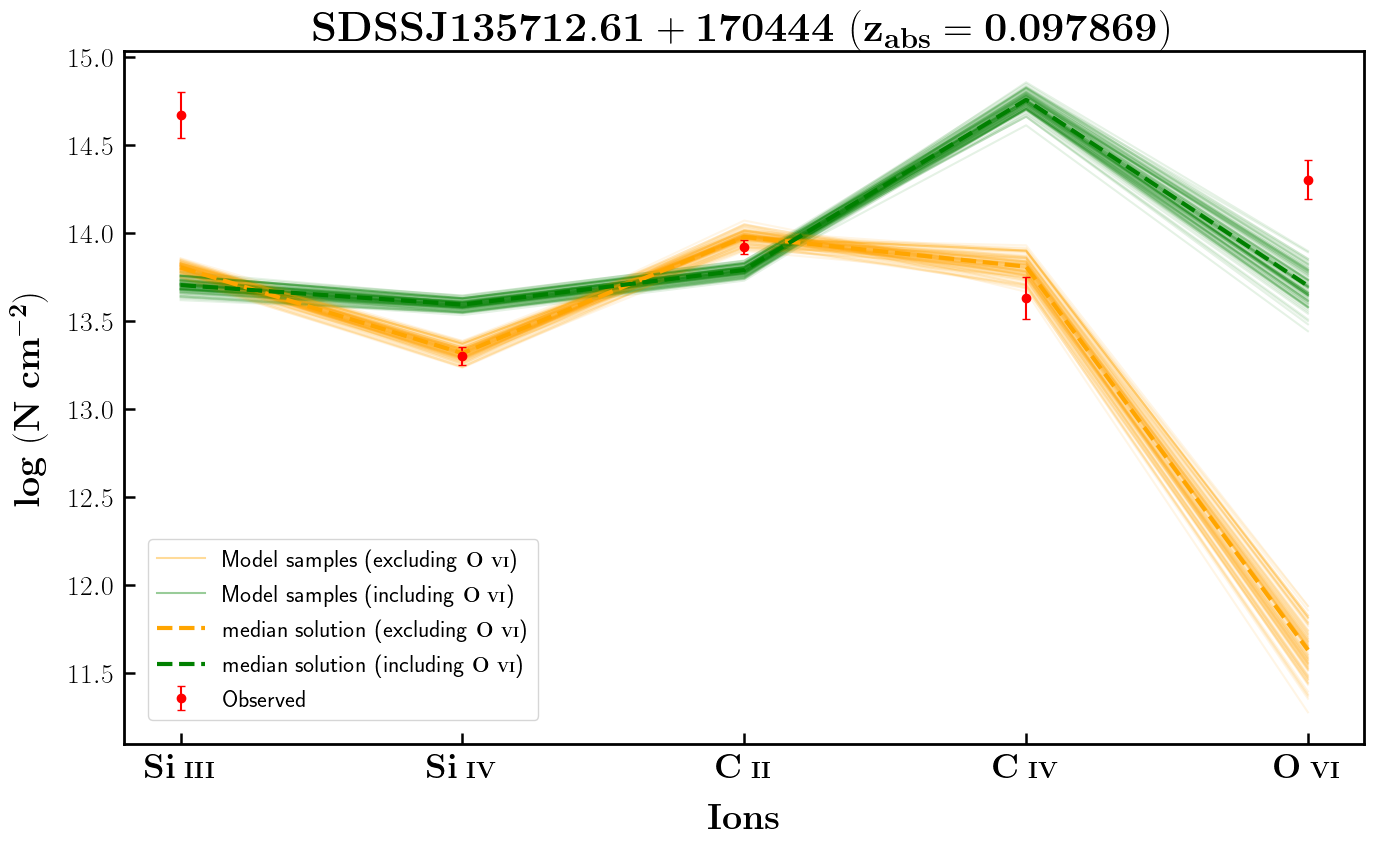
\includegraphics[width=0.85\linewidth]{Ionisation-Modelling-Plots/s135712-z=0.097869-compIII_logZ=-1.png}
    \caption{N(\ion{H}{i})=15.01, log $Z_{ref}$=-1}
\end{figure}

\newpage

\begin{figure}[!h]
    \centering
    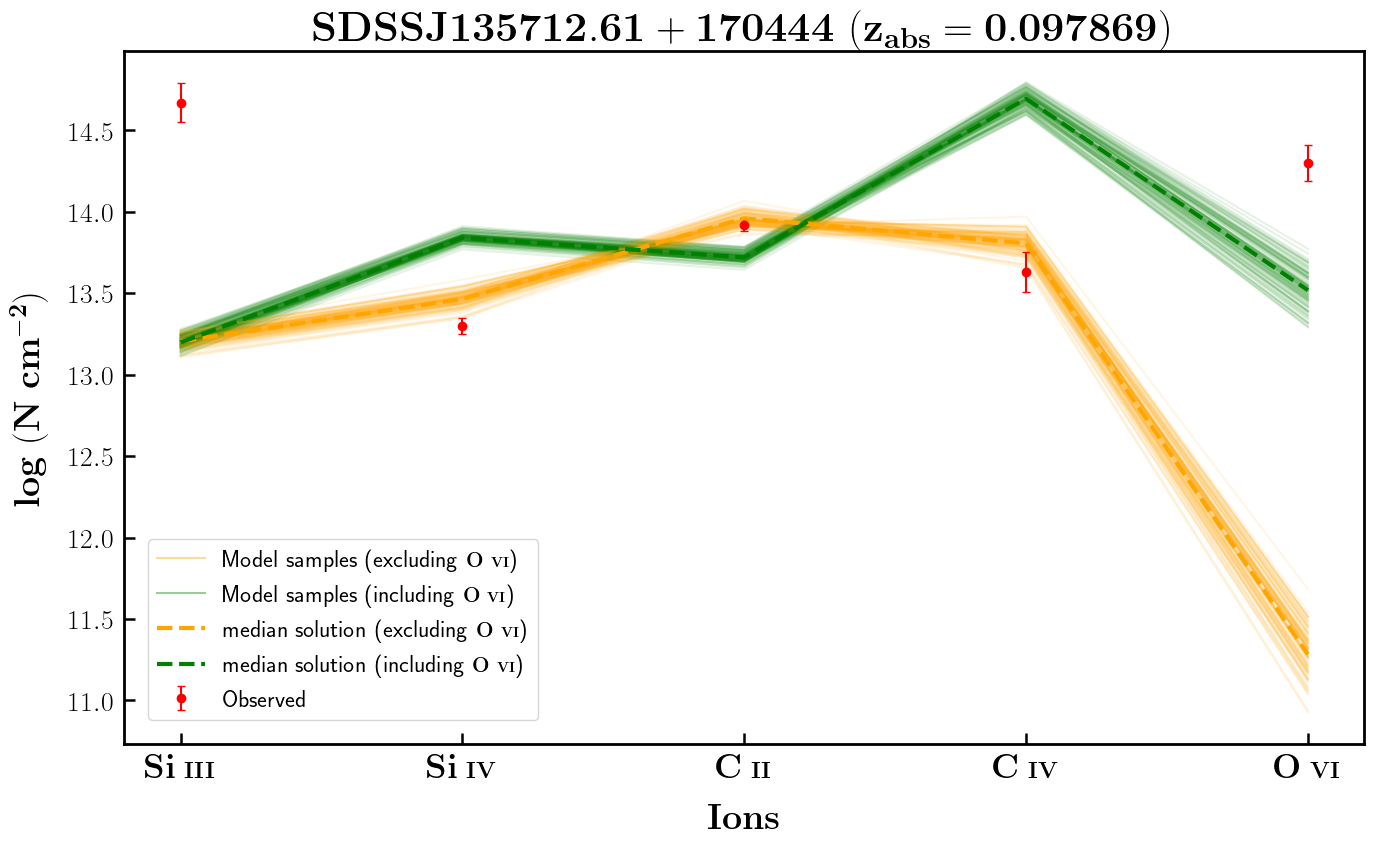
\includegraphics[width=0.85\linewidth]{Ionisation-Modelling-Plots/s135712-z=0.097869-compIII_logZ=1.png}
    \caption{N(\ion{H}{i})=15.01, log $Z_{ref}$=1}
\end{figure}


\newpage

\textbf{Non-detections}

\begin{figure}[!h]
    \centering
    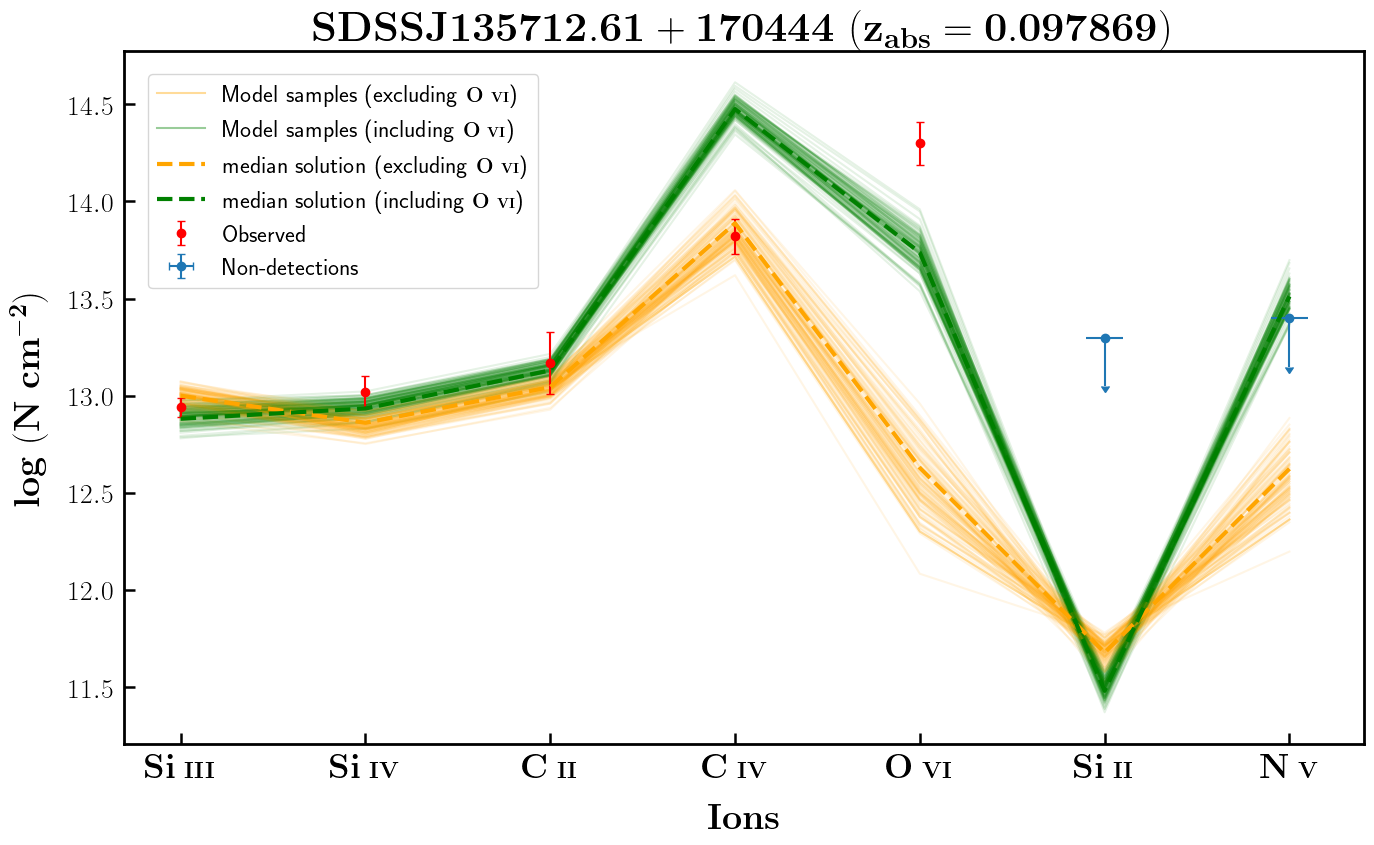
\includegraphics[width=0.85\linewidth]{Ionisation-Modelling-Plots/s135712-z=0.097869-compII_logZ=-1_non_detection.png}
    \caption{N(\ion{H}{i})=16.49, log $Z_{ref}$=-1}
\end{figure}

\begin{figure}[!h]
    \centering
    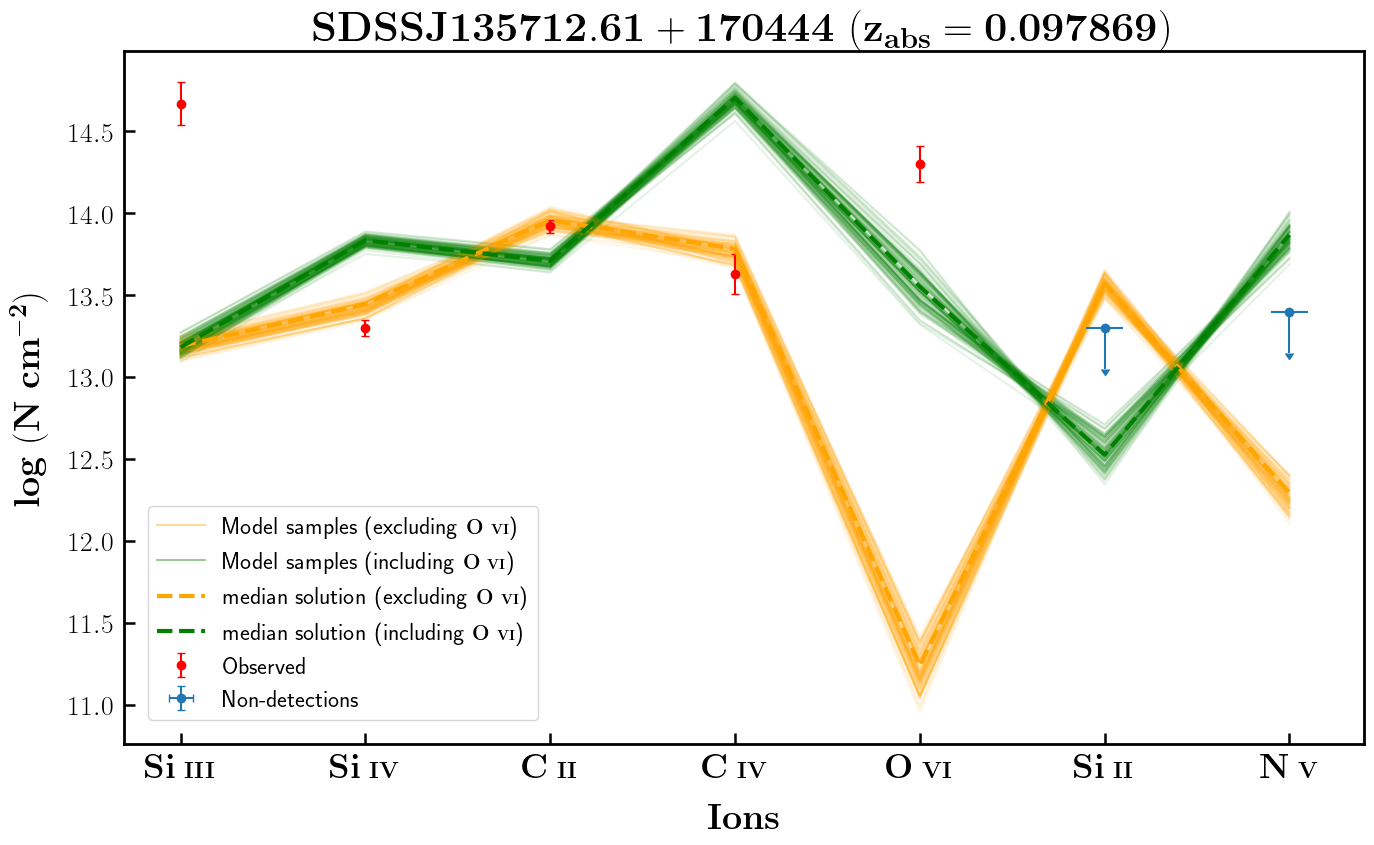
\includegraphics[width=0.85\linewidth]{Ionisation-Modelling-Plots/s135712-z=0.097869-compIII_logZ=1_non_detection.png}
    \caption{N(\ion{H}{i})=15.01, log $Z_{ref}$=1}
\end{figure}

\newpage

\textbf{Comments}
\\\\
\begin{itemize}
    \item Good solution II component (N(\ion{H}{i})=16.49) : small \emph{b} value - 29 km/s
    \item All other 4 ions could be explained together except \ion{O}{vi}
    \item When excluded \ion{O}{vi} is heavily underproduced
    \item For III component (N(\ion{H}{i})=15.01), model can't predict column density of \ion{Si}{iii} for the excluding \ion{O}{vi} case. 
    \item Ionisation : CI
    \item BLA : +ve
\end{itemize}


\newpage

\begin{landscape}

\begin{figure}
    \centering
    \vspace{-20mm}
    \hspace*{-35mm}
    \captionsetup{oneside,margin={0cm,35mm}}
    \includegraphics[width=1.25\linewidth]{System-Plots/1ES1553+113_z=0.187764_sys_plot.png}
\end{figure}

\end{landscape}


\begin{center} 

\begin{tabular}{cccc} 

    \hline \hline \tabularnewline 
    \head{Ion} & \head{v (km s\textsuperscript{$\mathbf{-1}$})} & \head{b (km s\textsuperscript{$\mathbf{-1}$})} & \head{log [N cm\textsuperscript{$\mathbf{-2}$}]}
    \tabularnewline \tabularnewline \hline \tabularnewline 
 
    \ion{C}{iii}   &    -46 $\pm$ 1    &    5 $\pm$ 4    &     13.17 $\pm$ 0.46 \\
    \ion{C}{iii}   &    -6 $\pm$ 1    &    13 $\pm$ 2    &     13.21 $\pm$ 0.03 \\
    \ion{N}{v}   &    -47 $\pm$ 2    &    17 $\pm$ 0    &     13.43 $\pm$ 0.05 \\
    \ion{N}{v}   &    -5 $\pm$ 2    &    16 $\pm$ 4    &     13.33 $\pm$ 0.06 \\
    \ion{O}{vi}   &    -42 $\pm$ 1    &    3 $\pm$ 1    &     14.23 $\pm$ 0.33 \\
    \ion{O}{vi}   &    0 $\pm$ 1    &    15 $\pm$ 3    &     13.71 $\pm$ 0.03 \\
    \ion{O}{vi}   &    511 $\pm$ 3    &    28 $\pm$ 5    &     13.49 $\pm$ 0.05 \\
    \ion{H}{i}   &    -52 $\pm$ 3    &    8 $\pm$ 6    &     12.76 $\pm$ 0.15 \\
    \ion{H}{i}   &    -28 $\pm$ 1    &    51 $\pm$ 1    &     13.88 $\pm$ 0.01 \\
    \ion{H}{i}   &    425 $\pm$ 3    &    25 $\pm$ 5    &     13.02 $\pm$ 0.07 \\
    \ion{H}{i}   &    496 $\pm$ 2    &    37 $\pm$ 3    &     13.46 $\pm$ 0.03 \\

    \tabularnewline \hline \hline \tabularnewline 

\end{tabular}

\end{center}

N(\ion{H}{I})=12.76 \\

Excluding \ion{O}{vi} : $n_H$ = -4.62 $\pm$ 0.04 \hspace{10mm} $Z$ = 1.37 $\pm$ 0.06

Including \ion{O}{vi} : $n_H$ = -4.63 $\pm$ 0.03 \hspace{10mm} $Z$ = 1.37 $\pm$ 0.06
\\\\
NOTE : Reference metallicity at log Z = 1. Low N(\ion{H}{I}), and error for column density for \ion{C}{iii} and \ion{O}{vi} for component I were obtained from $\chi^2$, else they were large and convergence was not good. Nearly similar solution for both the cases. \\

N(\ion{H}{I})=13.88 \\

Excluding \ion{O}{vi} : $n_H$ = -4.6 $\pm$ 0.04 \hspace{10mm} $Z$ = 0.03 $\pm$ 0.03

Including \ion{O}{vi} : $n_H$ = -4.44 $\pm$ 0.02 \hspace{10mm} $Z$ = -0.06 $\pm$ 0.02
\\\\


\newpage


\begin{figure}[!h]
    \centering
    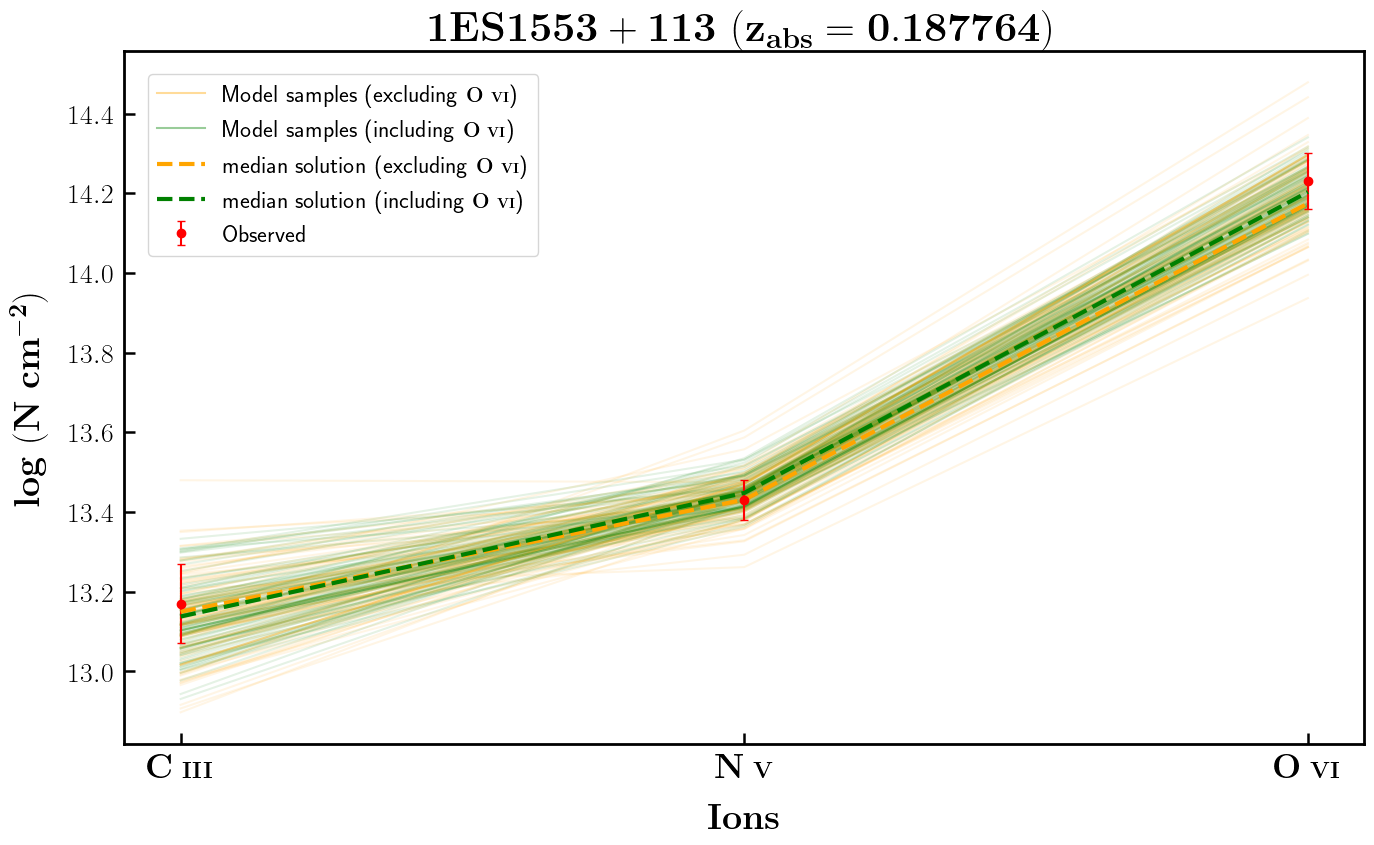
\includegraphics[width=0.85\linewidth]{Ionisation-Modelling-Plots/1es1553-z=0.187764-compI.png}
    \caption{N(\ion{H}{i})=12.76}
\end{figure}

\begin{figure}[!b]
    \centering
    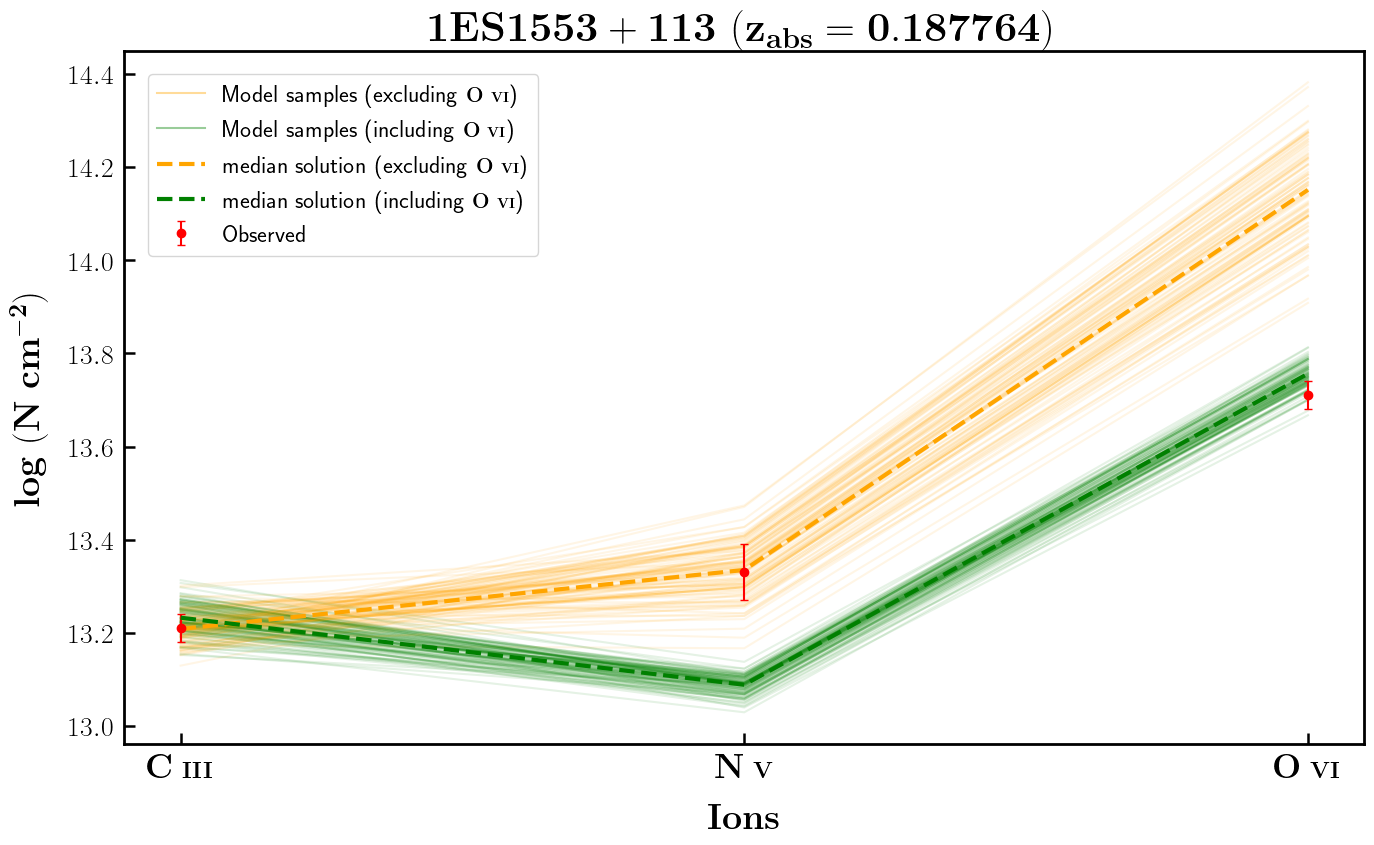
\includegraphics[width=0.85\linewidth]{Ionisation-Modelling-Plots/1es1553-z=0.187764-compII.png}
    \caption{N(\ion{H}{i})=13.88}
\end{figure}


\newpage

\textbf{Non-detections}

\begin{figure}[!h]
    \centering
    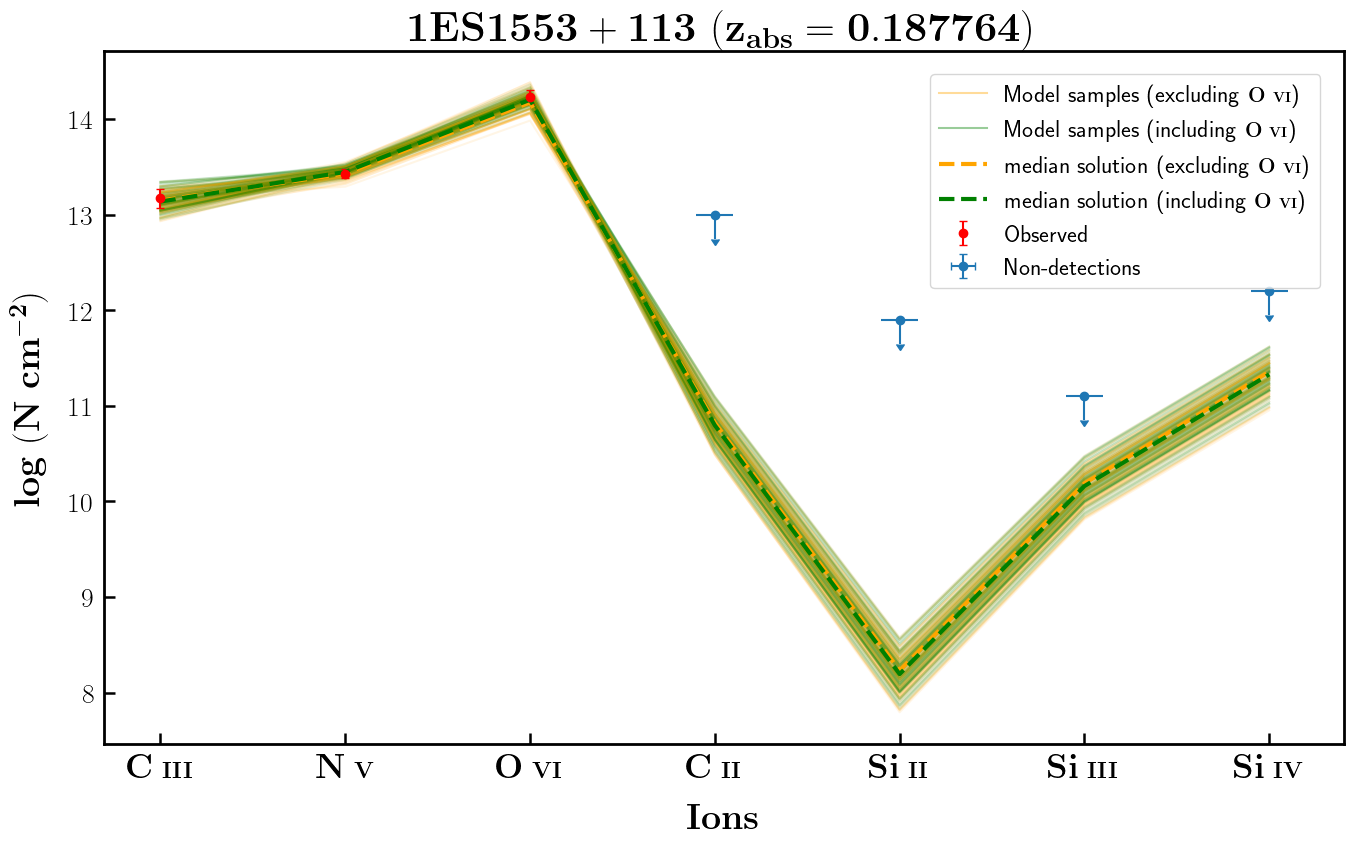
\includegraphics[width=0.8\linewidth]{Ionisation-Modelling-Plots/1es1553-z=0.187764-compI_logZ=1_non_detection.png}
    \caption{N(\ion{H}{i})=12.76, log $Z_{ref}$=1}
\end{figure}

\begin{figure}[!h]
    \centering
    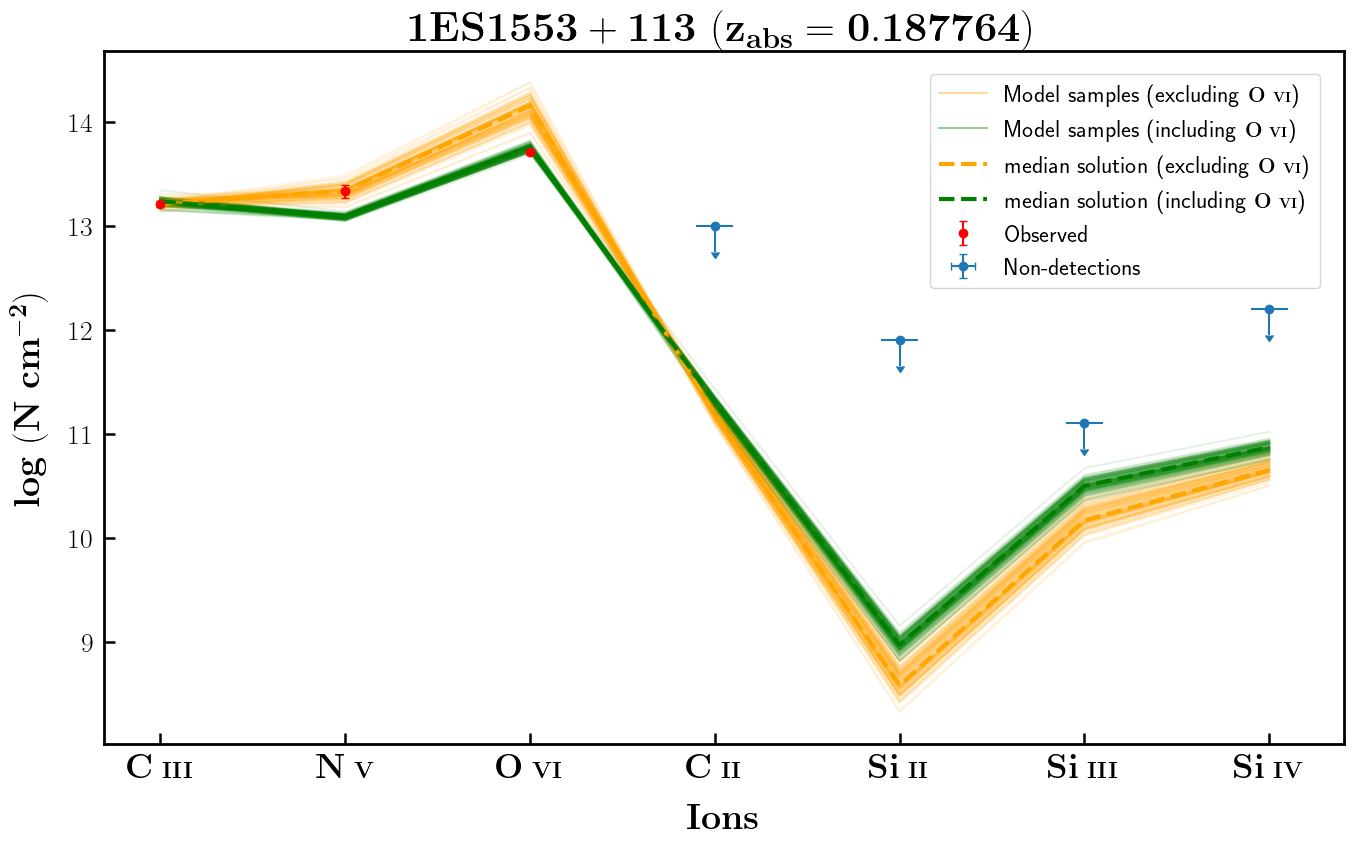
\includegraphics[width=0.8\linewidth]{Ionisation-Modelling-Plots/1es1553-z=0.187764-compII_logZ=-1_non_detection.png}
    \caption{N(\ion{H}{i})=13.88, log $Z_{ref}$=-1}
\end{figure}


\newpage

\textbf{Comments}
\\\\
\begin{itemize}
    \item Same solution for  I component (N(\ion{H}{i})=12.76) : all ions explained in both the cases : PI
    \item For II component (N(\ion{H}{i})=13.02), all 3 ions couldn't be explained together, \ion{O}{vi} is overproduced. 
    \item Ionisation : PI in component I and CI for component II
    \item BLA : +ve
\end{itemize}



\newpage

\begin{landscape}

\begin{figure}
    \centering
    \vspace{-20mm}
    \hspace*{-35mm}
    \captionsetup{oneside,margin={0cm,35mm}}
    \includegraphics[width=1.25\linewidth]{System-Plots/SBS1108+560_z=0.463207_sys_plot.png}
\end{figure}

\end{landscape}


\begin{center} 

\begin{tabular}{cccc} 

    \hline \hline \tabularnewline 
    \head{Ion} & \head{v (km s\textsuperscript{$\mathbf{-1}$})} & \head{b (km s\textsuperscript{$\mathbf{-1}$})} & \head{log [N cm\textsuperscript{$\mathbf{-2}$}]}
    \tabularnewline \tabularnewline \hline \tabularnewline 
 
    \ion{O}{i}   &    25 $\pm$ 2    &    18 $\pm$ 4    &     14.13 $\pm$ 0.05 \\
    \ion{Si}{iii}   &    -23 $\pm$ 9    &    39 $\pm$ 12    &     13.26 $\pm$ 0.12 \\
    \ion{Si}{iii}   &    21 $\pm$ 2    &    13 $\pm$ 15    &     14.61 $\pm$ 0.24 \\
    \ion{C}{ii}   &    12 $\pm$ 9    &    31 $\pm$ 4    &     14.15 $\pm$ 0.05 \\
    \ion{C}{ii}   &    34 $\pm$ 2    &    12 $\pm$ 5    &     14.67 $\pm$ 0.1 \\
    \ion{C}{iii}   &    -48 $\pm$ 3    &    15 $\pm$ 1    &     13.66 $\pm$ 0.08 \\
    \ion{C}{iii}   &    -10 $\pm$ 3    &    26 $\pm$ 7    &     14.16 $\pm$ 0.07 \\
    \ion{C}{iii}   &    28 $\pm$ 3    &    24 $\pm$ 1    &     13.95 $\pm$ 0.05 \\
    \ion{N}{iii}   &    -22 $\pm$ 59    &    67 $\pm$ 61    &     13.77 $\pm$ 0.1 \\
    \ion{N}{iii}   &    32 $\pm$ 2    &    26 $\pm$ 4    &     14.49 $\pm$ 0.09 \\
    \ion{Si}{ii}   &    25 $\pm$ 1    &    15 $\pm$ 1    &     13.57 $\pm$ 0.08 \\
    \ion{O}{vi}   &    0 $\pm$ 6    &    45 $\pm$ 10    &     13.71 $\pm$ 0.07 \\
    \ion{H}{i}   &    -48 $\pm$ 0    &    22 $\pm$ 2    &     15.77 $\pm$ 0.02 \\
    \ion{H}{i}   &    -10 $\pm$ 2    &    16 $\pm$ 0    &     15.79 $\pm$ 0.11 \\
    \ion{H}{i}   &    28 $\pm$ 1    &    16 $\pm$ 1    &     18.1 $\pm$ 0.12 \\
    
    \tabularnewline \hline \hline \tabularnewline 

\end{tabular}

\end{center}

log $Z_{ref}$=-1

N(\ion{H}{I})=18.10 \\

Excluding \ion{O}{vi} : $n_H$ = -1.88 $\pm$ 0.03 \hspace{10mm} $Z$ = 1.07 $\pm$ 0.04

Including \ion{O}{vi} : $n_H$ = -2.83 $\pm$ 0.02 \hspace{10mm} $Z$ = 0.89 $\pm$ 0.03
\\\\
NOTE : Using \ion{O}{vi} from other component to compare
\\\\
N(\ion{H}{I})=15.79 \\

Excluding \ion{O}{vi} : $n_H$ = -2.65 $\pm$ 0.22 \hspace{10mm} $Z$ = 1.6 $\pm$ 0.22

Including \ion{O}{vi} : $n_H$ = -3.56 $\pm$ 0.03 \hspace{10mm} $Z$ = 1.16 $\pm$ 0.05
\\\\

log $Z_{ref}$=1

N(\ion{H}{I})=18.10   \\ 

Excluding \ion{O}{vi} : $n_H$ = -2.55 $\pm$ 0.03 \hspace{10mm} $Z$ = -0.83 $\pm$ 0.04

Including \ion{O}{vi} : $n_H$ = -3.49 $\pm$ 0.01 \hspace{10mm} $Z$ = -0.92 $\pm$ 0.03
\\\\
N(\ion{H}{I})=15.79   \\ 

Excluding \ion{O}{vi} : $n_H$ = -3.33 $\pm$ 0.10 \hspace{10mm} $Z$ = -0.02 $\pm$ 0.12

Including \ion{O}{vi} : $n_H$ = -3.99 $\pm$ 0.02 \hspace{10mm} $Z$ = -0.44 $\pm$ 0.05
\\\\
NOTE : With log $Z_{ref}=1$, logZ is coming -ve for both the components



\newpage

\begin{figure}[!h]
    \centering
    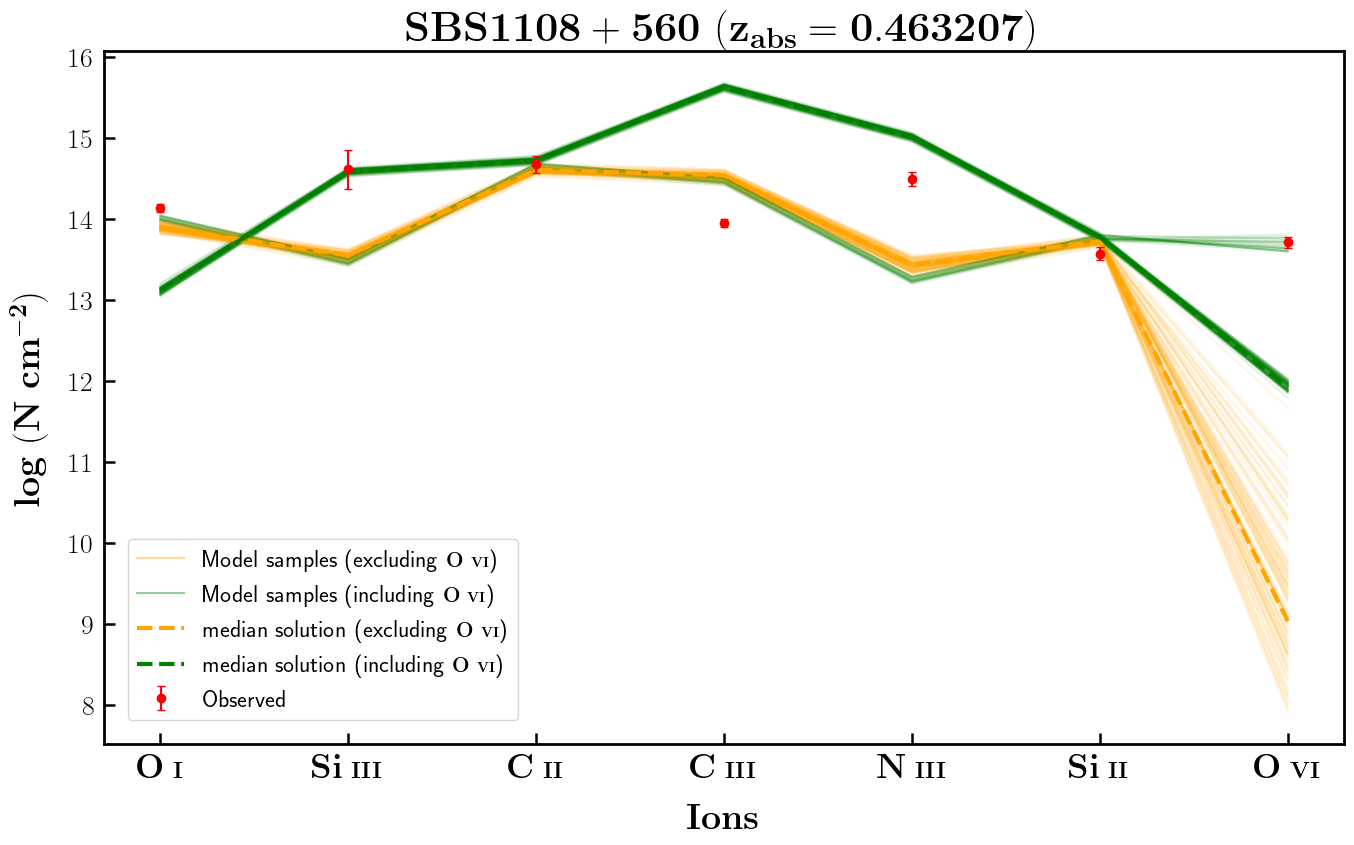
\includegraphics[width=0.85\linewidth]{Ionisation-Modelling-Plots/sbs1108-z=0.463207-compIII_logZ=-1.png}
    \caption{N(\ion{H}{i})=18.10, log $Z_{ref}$=-1}
\end{figure}


\begin{figure}[!b]
    \centering
    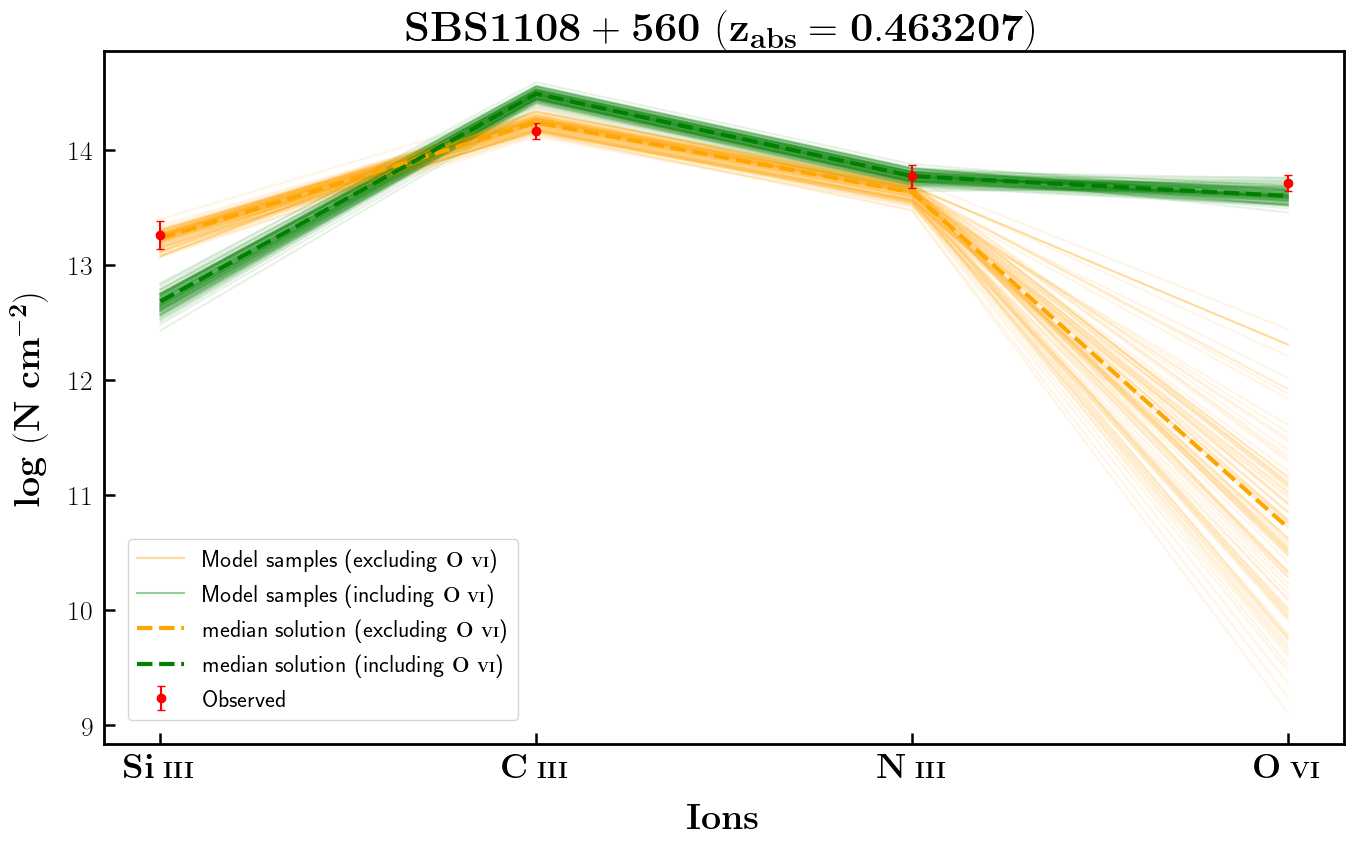
\includegraphics[width=0.85\linewidth]{Ionisation-Modelling-Plots/sbs1108-z=0.463207-compII_logZ=-1.png}
    \caption{N(\ion{H}{i})=15.79, log $Z_{ref}$=-1}
\end{figure}

\newpage

\begin{figure}[!h]
    \centering
    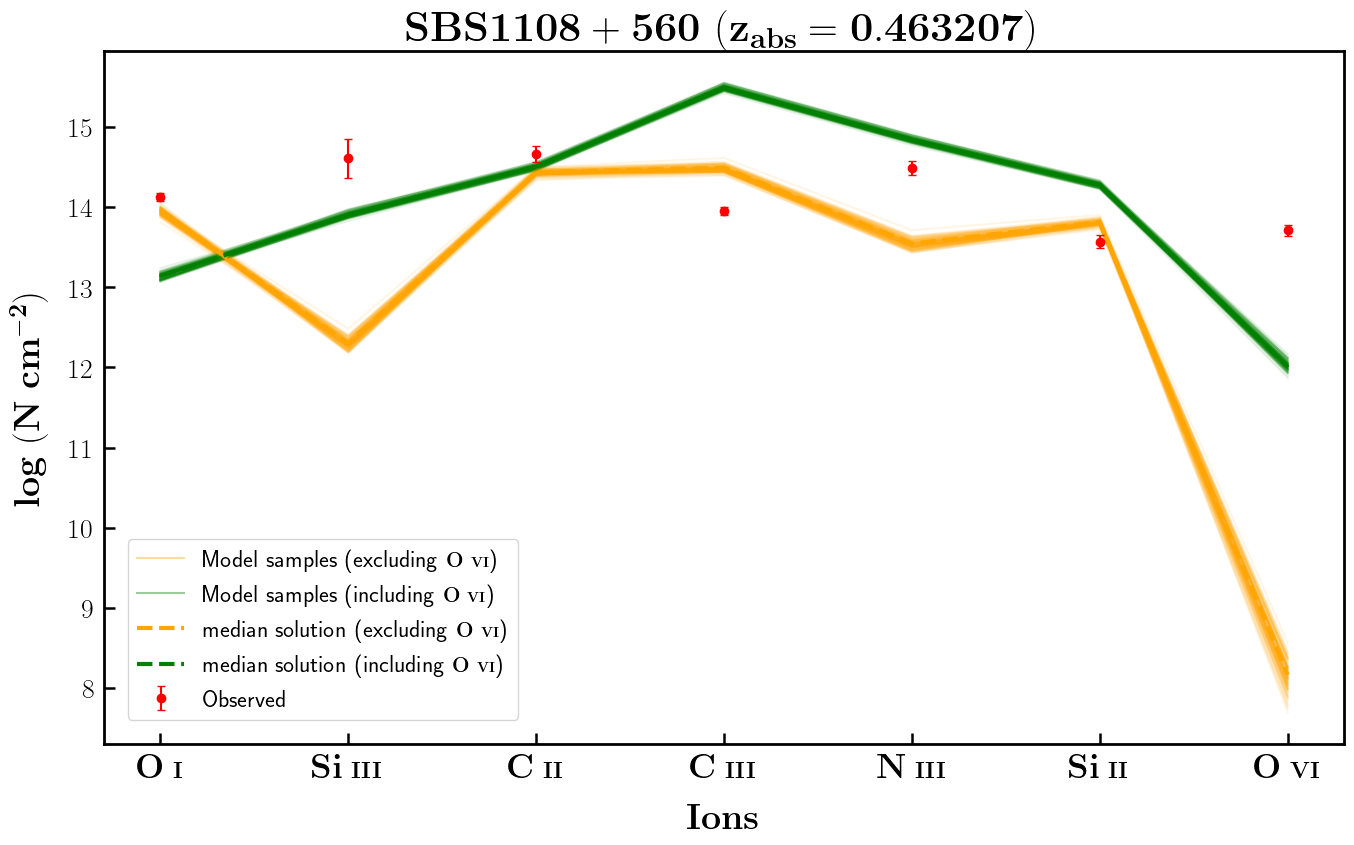
\includegraphics[width=0.85\linewidth]{Ionisation-Modelling-Plots/sbs1108-z=0.463207-compIII_logZ=1.png}
    \caption{N(\ion{H}{i})=18.10, log $Z_{ref}$=1}
\end{figure}


\begin{figure}[!b]
    \centering
    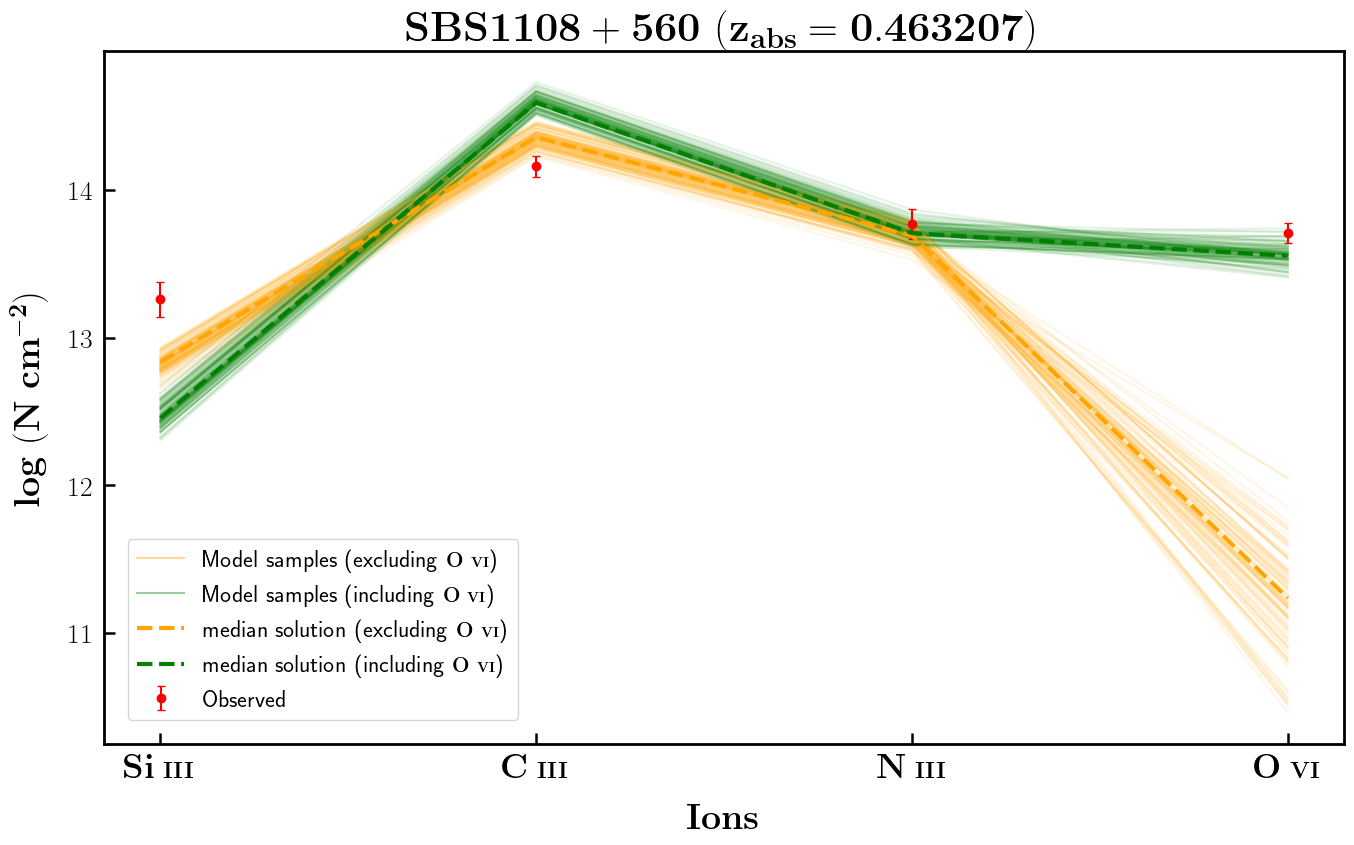
\includegraphics[width=0.85\linewidth]{Ionisation-Modelling-Plots/sbs1108-z=0.463207-compII_logZ=1.png}
    \caption{N(\ion{H}{i})=15.79, log $Z_{ref}$=1}
\end{figure}


\newpage

\textbf{Comments}
\\\\
\begin{itemize}
    \item Smaller \emph{b} values for all 3 components
    \item Not much good solution for component III ((N(\ion{H}{i})=18.10)), as there are many ions. Only few can be explained.
    \item Modelled using both logZ=-1 and logZ=1 for both the components
    \item For component II ((N(\ion{H}{i})=15.79)), when using logZ=1 model, the metallicity is coming -ve. And the solution is better when logZ=-1 model is used.
    \item Ionisation : CI
    \item BLA : tentative
\end{itemize}



\newpage

\begin{landscape}

\begin{figure}
    \centering
    \vspace{-20mm}
    \hspace*{-35mm}
    \captionsetup{oneside,margin={0cm,35mm}}
    \includegraphics[width=1.25\linewidth]{System-Plots/PG1222+216_z=0.378389_sys_plot.png}
\end{figure}

\end{landscape}


\begin{center} 

\begin{tabular}{cccc} 

    \hline \hline \tabularnewline 
    \head{Ion} & \head{v (km s\textsuperscript{$\mathbf{-1}$})} & \head{b (km s\textsuperscript{$\mathbf{-1}$})} & \head{log [N cm\textsuperscript{$\mathbf{-2}$}]}
    \tabularnewline \tabularnewline \hline \tabularnewline 
 
    \ion{O}{iii}   &    7 $\pm$ 5    &    61 $\pm$ 8    &     14.51 $\pm$ 0.04 \\
    \ion{Si}{iii}   &    0 $\pm$ 2    &    30 $\pm$ 3    &     12.98 $\pm$ 0.03 \\
    \ion{C}{iii}   &    -261 $\pm$ 3    &    17 $\pm$ 5    &     13.54 $\pm$ 0.06 \\
    \ion{C}{iii}   &    -215 $\pm$ 5    &    22 $\pm$ 6    &     13.40 $\pm$ 0.08 \\
    \ion{C}{iii}   &    0 $\pm$ 2    &    32 $\pm$ 3    &     13.79 $\pm$ 0.02 \\
    \ion{C}{iii}   &    63 $\pm$ 3    &    13 $\pm$ 6    &     13.12 $\pm$ 0.07 \\
    \ion{O}{vi}   &    -439 $\pm$ 3    &    28 $\pm$ 5    &     13.42 $\pm$ 0.06 \\
    \ion{O}{vi}   &    -264 $\pm$ 6    &    24 $\pm$ 6    &     13.75 $\pm$ 0.2 \\
    \ion{O}{vi}   &    -223 $\pm$ 14    &    34 $\pm$ 13    &     13.68 $\pm$ 0.24 \\
    \ion{O}{vi}   &    -24 $\pm$ 12    &    14 $\pm$ 18    &     13.00 $\pm$ 0.11 \\
    \ion{O}{vi}   &    13 $\pm$ 4    &    29 $\pm$ 13    &     13.95 $\pm$ 0.16 \\
    \ion{O}{vi}   &    59 $\pm$ 6    &    18 $\pm$ 7    &     13.42 $\pm$ 0.23 \\
    \ion{H}{i}   &    -455 $\pm$ 3    &    26 $\pm$ 4    &     13.40 $\pm$ 0.06 \\
    \ion{H}{i}   &    -353 $\pm$ 9    &    64 $\pm$ 19    &     13.54 $\pm$ 0.11 \\
    \ion{H}{i}   &    -268 $\pm$ 1    &    16 $\pm$ 6    &     13.70 $\pm$ 0.14 \\
    \ion{H}{i}   &    -227 $\pm$ 5    &    52 $\pm$ 4    &     14.34 $\pm$ 0.05 \\
    \ion{H}{i}   &    -27 $\pm$ 2    &    23 $\pm$ 1    &     14.73 $\pm$ 0.08 \\
    \ion{H}{i}   &    31 $\pm$ 2    &    43 $\pm$ 1    &     15.43 $\pm$ 0.04 \\
    
    \tabularnewline \hline \hline \tabularnewline 

\end{tabular}

\end{center}

N(\ion{H}{I})=15.43 \\

Excluding \ion{O}{vi} : $n_H$ = -2.66 $\pm$ 0.05 \hspace{10mm} $Z$ = -0.25 $\pm$ 0.06

Including \ion{O}{vi} : $n_H$ = -3.16 $\pm$ 0.03 \hspace{10mm} $Z$ = -0.66 $\pm$ 0.02
\\\\
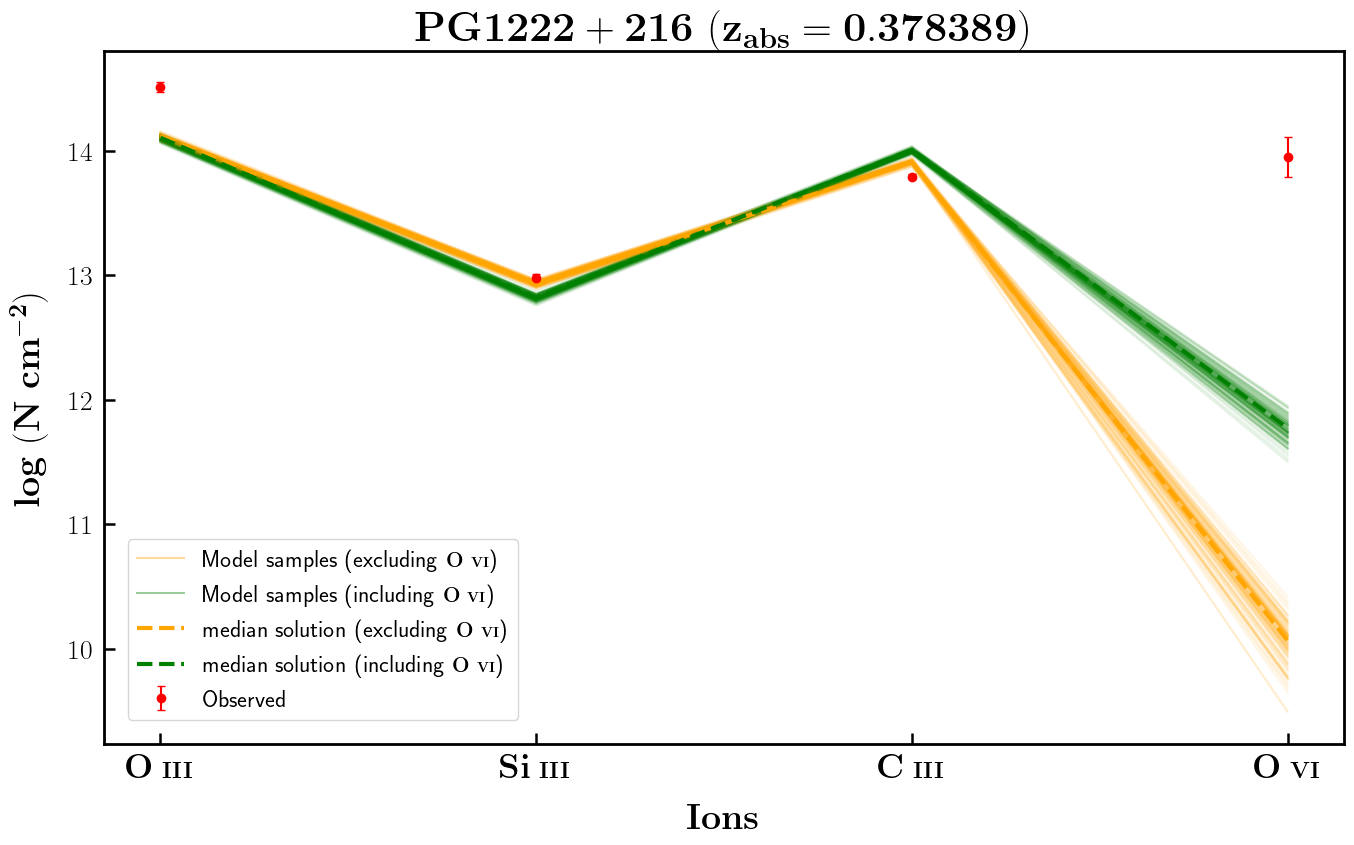
\includegraphics[width=1\linewidth]{Ionisation-Modelling-Plots/pg1222-z=0.378389-compVI.png}


\newpage

\textbf{Comments}
\\\\
\begin{itemize}
    \item All ions couldn't be xplained together
    \item When excluded, \ion{O}{vi} is underproduced. However, column density of \ion{O}{iii} is also off by around 0.5 dex from predicted value 
    \item Ionisation : CI
    \item BLA : +ve
\end{itemize}


\newpage

\begin{landscape}

\begin{figure}
    \centering
    \vspace{-20mm}
    \hspace*{-35mm}
    \captionsetup{oneside,margin={0cm,35mm}}
    \includegraphics[width=1.25\linewidth]{System-Plots/PG1116+215_z=0.138527_sys_plot.png}
\end{figure}

\end{landscape}


\begin{center} 

\begin{tabular}{cccc} 

    \hline \hline \tabularnewline 
    \head{Ion} & \head{v (km s\textsuperscript{$\mathbf{-1}$})} & \head{b (km s\textsuperscript{$\mathbf{-1}$})} & \head{log [N cm\textsuperscript{$\mathbf{-2}$}]}
    \tabularnewline \tabularnewline \hline \tabularnewline 
 
    \ion{N}{v}   &    -7 $\pm$ 3    &    12 $\pm$ 6    &     12.84 $\pm$ 0.09 \\
    \ion{N}{ii}   &    -5 $\pm$ 1    &    6 $\pm$ 3    &     13.62 $\pm$ 0.11 \\
    \ion{N}{ii}   &    33 $\pm$ 6    &    8 $\pm$ 13    &     12.85 $\pm$ 0.15 \\
    \ion{P}{ii}   &    -44 $\pm$ 5    &    19 $\pm$ 8    &     12.94 $\pm$ 0.09 \\
    \ion{Si}{ii}   &    -13 $\pm$ 1    &    9 $\pm$ 1    &     12.46 $\pm$ 0.06 \\
    \ion{Si}{ii}   &    13 $\pm$ 1    &    23 $\pm$ 3    &     12.31 $\pm$ 0.04 \\
    \ion{Si}{iii}   &    -9 $\pm$ 1    &    10 $\pm$ 1    &     12.92 $\pm$ 0.04 \\
    \ion{Si}{iv}   &    -13 $\pm$ 2    &    4 $\pm$ 3    &     12.84 $\pm$ 0.09 \\
    \ion{O}{vi}   &    -1 $\pm$ 1    &    35 $\pm$ 3    &     13.84 $\pm$ 0.02 \\
    \ion{C}{iv}   &    -10 $\pm$ 3    &    13 $\pm$ 4    &     13.17 $\pm$ 0.07 \\
    \ion{C}{ii}   &    -7 $\pm$ 1    &    9 $\pm$ 1    &     13.85 $\pm$ 0.04 \\
    \ion{H}{i}   &    -8 $\pm$ 3    &    27 $\pm$ 2    &     14.97 $\pm$ 0.05 \\
    \ion{H}{i}   &    -5 $\pm$ 9    &    71 $\pm$ 14    &     13.6 $\pm$ 0.23 \\
    \ion{H}{i}   &    31 $\pm$ 2    &    6 $\pm$ 2    &     16.04 $\pm$ 1.77 \\

    \tabularnewline \hline \hline \tabularnewline 

\end{tabular}

\end{center}

N(\ion{H}{I})=13.60   \\ 

log $Z_{ref}=-1$ \\

Excluding \ion{O}{vi} : $n_H$ = -3.24 $\pm$ 0.03 \hspace{10mm} $Z$ = 1.92 $\pm$ 0.03

Including \ion{O}{vi} : $n_H$ = -3.88 $\pm$ 0.01 \hspace{10mm} $Z$ = 1.87 $\pm$ 0.02 \\
\\\\
log $Z_{ref}=1$ \\

Excluding \ion{O}{vi} : $n_H$ = -3.92 $\pm$ 0.02 \hspace{10mm} $Z$ = 2.0 $\pm$ 0.0

Including \ion{O}{vi} : $n_H$ = -4.35 $\pm$ 0.0 \hspace{10mm} $Z$ = 2.0 $\pm$ 0.0

NOTE : logZ coming near 2 for both the cases and for logZ=1 also, \ion{P}{ii} is not Included

\newpage 

\begin{figure}[!h]
    \centering
    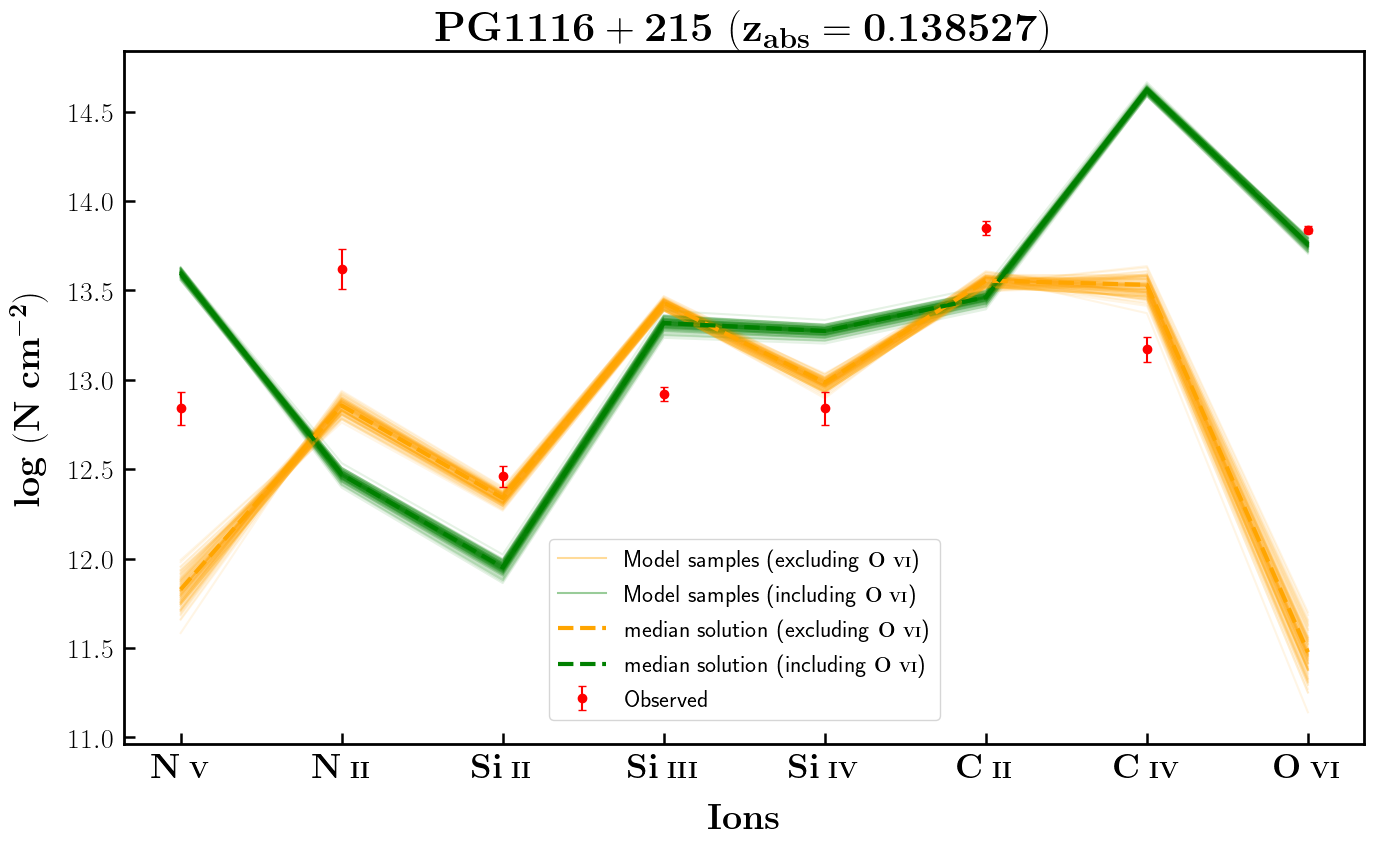
\includegraphics[width=0.85\linewidth]{Ionisation-Modelling-Plots/pg1116-z=0.138527-compII_logZ=-1.png}
    \caption{N(\ion{H}{i})=13.60, log $Z_{ref}=-1$}
\end{figure}

\begin{figure}[!b]
    \centering
    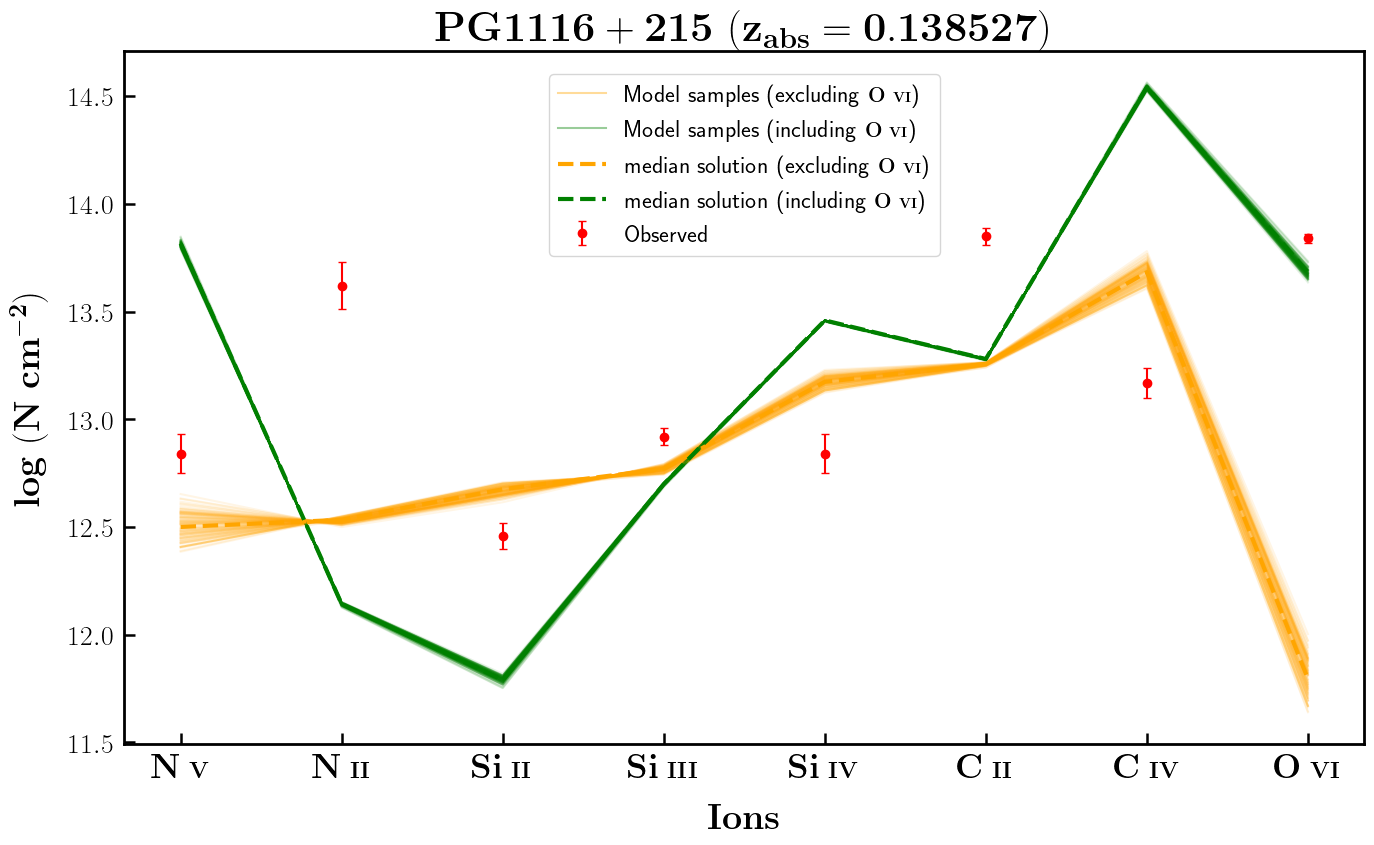
\includegraphics[width=0.85\linewidth]{Ionisation-Modelling-Plots/pg1116-z=0.138527-compII_logZ=1.png}
    \caption{N(\ion{H}{i})=13.60, log $Z_{ref}=1$}
\end{figure}


\newpage

\textbf{Comments}
\\\\
\begin{itemize}
    \item Not good solution as there are many ions.
    \item metallicity is coming 2, which is the upper bound taken in flat priors
    \item Ionisation : tentative CI (since \ion{O}{vi} can't be explained, even though the solution is not good)
    \item BLA : +ve
\end{itemize}



\newpage

\begin{landscape}

\begin{figure}
    \centering
    \vspace{-20mm}
    \hspace*{-35mm}
    \captionsetup{oneside,margin={0cm,35mm}}
    \includegraphics[width=1.25\linewidth]{System-Plots/H1821+643_z=0.170006_sys_plot.png}
\end{figure}

\end{landscape}


\begin{center} 

\begin{tabular}{cccc} 

    \hline \hline \tabularnewline 
    \head{Ion} & \head{v (km s\textsuperscript{$\mathbf{-1}$})} & \head{b (km s\textsuperscript{$\mathbf{-1}$})} & \head{log [N cm\textsuperscript{$\mathbf{-2}$}]}
    \tabularnewline \tabularnewline \hline \tabularnewline 
 
    \ion{Si}{iii}   &    7 $\pm$ 3    &    17 $\pm$ 5    &     12.05 $\pm$ 0.07 \\
    \ion{Si}{iii}   &    52 $\pm$ 6    &    14 $\pm$ 10    &     11.62 $\pm$ 0.17 \\
    \ion{N}{v}   &    47 $\pm$ 3    &    31 $\pm$ 5    &     13.29 $\pm$ 0.05 \\
    \ion{N}{v}   &    122 $\pm$ 7    &    21 $\pm$ 11    &     12.74 $\pm$ 0.14 \\
    \ion{O}{vi}   &    3 $\pm$ 28    &    152 $\pm$ 20    &     13.94 $\pm$ 0.06 \\
    \ion{O}{vi}   &    107 $\pm$ 9    &    48 $\pm$ 12    &     13.29 $\pm$ 0.11 \\
    \ion{H}{i}   &    -92 $\pm$ 1    &    36 $\pm$ 1    &     13.85 $\pm$ 0.02 \\
    \ion{H}{i}   &    0 $\pm$ 2    &    63 $\pm$ 3    &     13.68 $\pm$ 0.02 \\
    \ion{H}{i}   &    120 $\pm$ 1    &    28 $\pm$ 1    &     13.35 $\pm$ 0.02 \\

    \tabularnewline \hline \hline \tabularnewline 

\end{tabular}

\end{center}

log $Z_{ref}$ = -1

N(\ion{H}{I})= 13.68  \\ 

Excluding \ion{O}{vi} : $n_H$ = -4.10 $\pm$ 0.02 \hspace{10mm} $Z$ = 0.91 $\pm$ 0.04

Including \ion{O}{vi} : $n_H$ = -4.14 $\pm$ 0.02 \hspace{10mm} $Z$ = 0.94 $\pm$ 0.04 \\

N(\ion{H}{I})= 13.35  \\ 

Excluding \ion{O}{vi} : $n_H$ = -4.07 $\pm$ 0.06 \hspace{10mm} $Z$ = 0.75 $\pm$ 0.11

Including \ion{O}{vi} : $n_H$ = -4.11 $\pm$ 0.05 \hspace{10mm} $Z$ = 0.79 $\pm$ 0.10 \\

log $Z_{ref}$ = 1

N(\ion{H}{I})= 13.68  \\ 

Excluding \ion{O}{vi} : $n_H$ = -4.33 $\pm$ 0.02 \hspace{10mm} $Z$ = 1.30 $\pm$ 0.05

Including \ion{O}{vi} : $n_H$ = -4.43 $\pm$ 0.01 \hspace{10mm} $Z$ = 1.25 $\pm$ 0.05
\\\\

N(\ion{H}{I})= 13.35  \\ 

Excluding \ion{O}{vi} : $n_H$ = -4.30 $\pm$ 0.05 \hspace{10mm} $Z$ = 1.18 $\pm$ 0.13

Including \ion{O}{vi} : $n_H$ = -4.41 $\pm$ 0.02 \hspace{10mm} $Z$ = 1.15 $\pm$ 0.12


\newpage

\begin{figure}[!h]
    \centering
    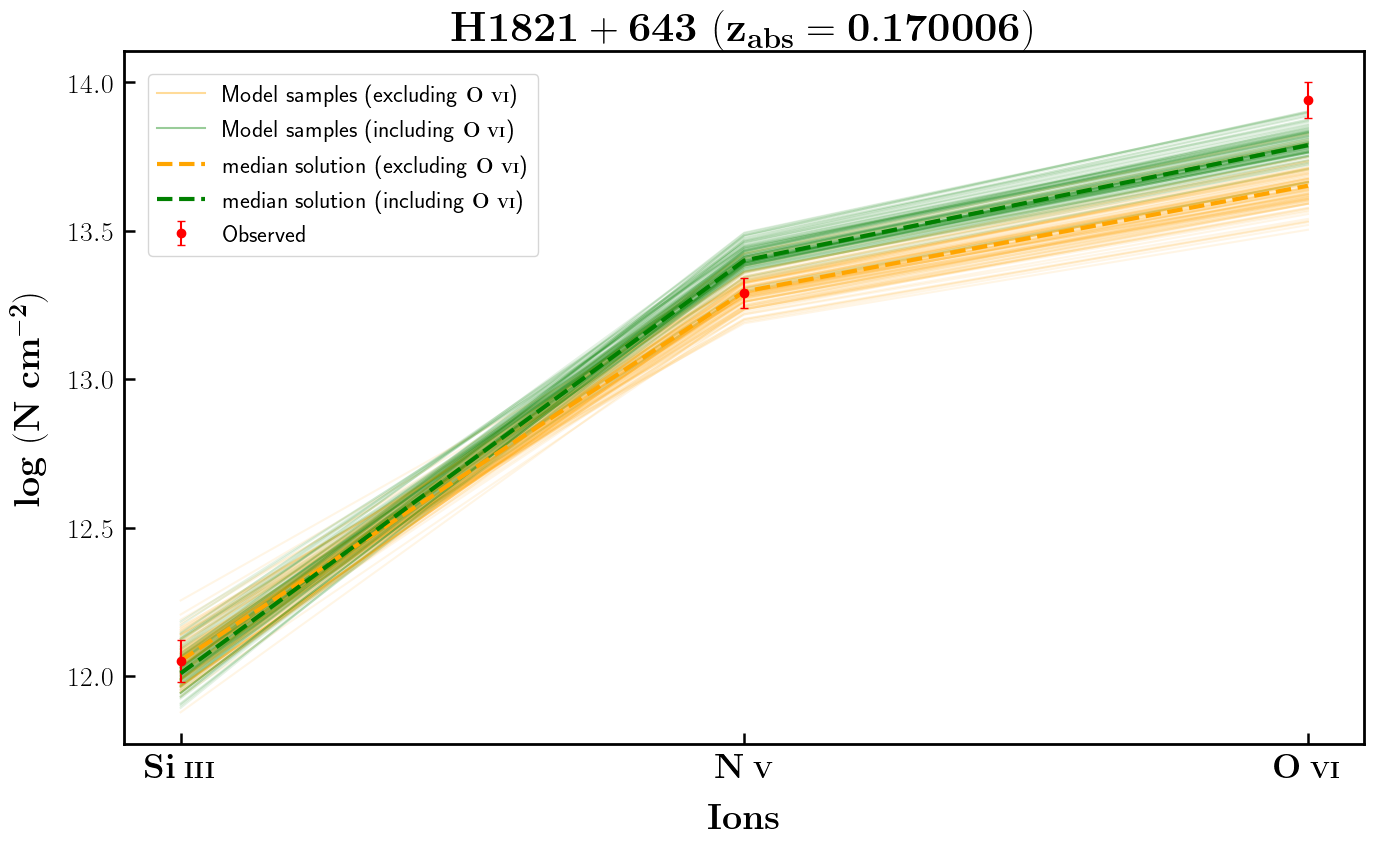
\includegraphics[width=0.85\linewidth]{Ionisation-Modelling-Plots/h1821-z=0.170006-compII_logZ=-1.png}
    \caption{N(\ion{H}{i})=13.68, log $Z_{ref}$ = -1}
\end{figure}

\begin{figure}[!b]
    \centering
    \includegraphics[width=0.85\linewidth]{Ionisation-Modelling-Plots/h1821-z=0.170006-compIII_logZ=-1.png}
    \caption{N(\ion{H}{i})=13.35, log $Z_{ref}$ = -1}
\end{figure}


\newpage

\begin{figure}[!h]
    \centering
    \includegraphics[width=0.85\linewidth]{Ionisation-Modelling-Plots/h1821-z=0.170006-compII.png}
    \caption{N(\ion{H}{i})=13.68, log $Z_{ref}$ = 1}
\end{figure}

\begin{figure}[!b]
    \centering
    \includegraphics[width=0.85\linewidth]{Ionisation-Modelling-Plots/h1821-z=0.170006-compIII.png}
    \caption{N(\ion{H}{i})=13.35, log $Z_{ref}$ = 1}
\end{figure}


\newpage

\textbf{Non-detections}

\begin{figure}[!h]
    \centering
    \includegraphics[width=0.85\linewidth]{Ionisation-Modelling-Plots/h1821-z=0.170006-compII_logZ=1_non_detection.png}
    \caption{N(\ion{H}{i})=13.68, log $Z_{ref}$=1}
\end{figure}

\begin{figure}[!h]
    \centering
    \includegraphics[width=0.85\linewidth]{Ionisation-Modelling-Plots/h1821-z=0.170006-compIII_logZ=1_non_detection.png}
    \caption{N(\ion{H}{i})=13.35, log $Z_{ref}$=1}
\end{figure}


\newpage

\textbf{Comments}
\\\\
\begin{itemize}
    \item For component II (N(\ion{H}{i})=13.68), solution very close to explaining all 3 ions but not exactly when using logZ=-1 models, but clearly, can't explain the 3 ions together when logZ=1 models are used.
    \item Similarly, for component III (N(\ion{H}{i})=13.68), all 3 ions can be explained when using logZ=-1 models, but not with logZ=1 models.
    \item Ionisation : CI
    \item BLA : +ve
\end{itemize}



\newpage

\begin{landscape}

\begin{figure}
    \centering
    \vspace{-20mm}
    \hspace*{-35mm}
    \captionsetup{oneside,margin={0cm,35mm}}
    \includegraphics[width=1.25\linewidth]{System-Plots/H1821+643_z=0.224981_sys_plot.png}
\end{figure}

\end{landscape}


\begin{center} 

\begin{tabular}{cccc} 

    \hline \hline \tabularnewline 
    \head{Ion} & \head{v (km s\textsuperscript{$\mathbf{-1}$})} & \head{b (km s\textsuperscript{$\mathbf{-1}$})} & \head{log [N cm\textsuperscript{$\mathbf{-2}$}]}
    \tabularnewline \tabularnewline \hline \tabularnewline 
 
    \ion{Si}{iii}   &    -59 $\pm$ 13    &    31 $\pm$ 18    &     12.23 $\pm$ 0.15 \\
    \ion{Si}{iii}   &    -1 $\pm$ 6    &    22 $\pm$ 9    &     12.71 $\pm$ 0.13 \\
    \ion{C}{iii}   &    -31 $\pm$ 1    &    24 $\pm$ 2    &     13.36 $\pm$ 0.07 \\
    \ion{C}{iii}   &    12 $\pm$ 1    &    36 $\pm$ 2    &     13.84 $\pm$ 0.02 \\
    \ion{C}{iii}   &    81 $\pm$ 3    &    15 $\pm$ 5    &     12.6 $\pm$ 0.09 \\
    \ion{C}{iii}   &    335 $\pm$ 7    &    20 $\pm$ 10    &     12.13 $\pm$ 0.11 \\
    \ion{O}{vi}   &    0 $\pm$ 1    &    45 $\pm$ 1    &     14.24 $\pm$ 0.01 \\
    \ion{O}{vi}   &    57 $\pm$ 2    &    3 $\pm$ 3    &     13.12 $\pm$ 0.1 \\
    \ion{O}{vi}   &    330 $\pm$ 1    &    13 $\pm$ 2    &     13.42 $\pm$ 0.03 \\
    \ion{H}{i}   &    -109 $\pm$ 3    &    33 $\pm$ 0    &     13.87 $\pm$ 0.09 \\
    \ion{H}{i}   &    -38 $\pm$ 1    &    30 $\pm$ 1    &     15.16 $\pm$ 0.02 \\
    \ion{H}{i}   &    -19 $\pm$ 10   &    84 $\pm$ 13    &     13.64 $\pm$ 0.11 \\
    \ion{H}{i}   &    18 $\pm$ 1    &    19 $\pm$ 1    &     15.13 $\pm$ 0.03 \\
    \ion{H}{i}   &    276 $\pm$ 7    &    62 $\pm$ 11    &     13.48 $\pm$ 0.06 \\
    
    \tabularnewline \hline \hline \tabularnewline 

\end{tabular}

\end{center}


N(\ion{H}{I})= 15.16  \\ 

Excluding \ion{O}{vi} : $n_H$ = -3.29 $\pm$ 0.08 \hspace{10mm} $Z$ = -0.95 $\pm$ 0.07

Including \ion{O}{vi} : $n_H$ = -4.36 $\pm$ 0.02 \hspace{10mm} $Z$ = -0.81 $\pm$ 0.04 \\

N(\ion{H}{I})= 15.13  \\ 

Excluding \ion{O}{vi} : $n_H$ = -3.29 $\pm$ 0.03 \hspace{10mm} $Z$ = -0.44 $\pm$ 0.03

Including \ion{O}{vi} : $n_H$ = -3.83 $\pm$ 0.04 \hspace{10mm} $Z$ = -0.77 $\pm$ 0.03 \\

NOTE : Solution using $\chi^2$, MCMC didn't converge good, shows hint of two solution, another solution with high density and metallicity for both the components


\newpage

\begin{figure}[!h]
    \centering
    \includegraphics[width=0.85\linewidth]{Ionisation-Modelling-Plots/h1821-z=0.224981-compII.png}
    \caption{N(\ion{H}{i})=15.16}
\end{figure}

\begin{figure}[!b]
    \centering
    \includegraphics[width=0.85\linewidth]{Ionisation-Modelling-Plots/h1821-z=0.224981-compIV.png}
    \caption{N(\ion{H}{i})=15.13}
\end{figure}


\newpage

\textbf{Non-detections}

\begin{figure}[!h]
    \centering
    \includegraphics[width=0.8\linewidth]{Ionisation-Modelling-Plots/h1821-z=0.224981-compII_logZ=-1_non_detection.png}
    \caption{N(\ion{H}{i})=15.16, log $Z_{ref}$=-1}
\end{figure}

\begin{figure}[!h]
    \centering
    \includegraphics[width=0.8\linewidth]{Ionisation-Modelling-Plots/h1821-z=0.224981-compIV_logZ=-1_non_detection.png}
    \caption{N(\ion{H}{i})=15.13, log $Z_{ref}$=-1}
\end{figure}




\newpage

\textbf{Comments}
\\\\
\begin{itemize}
    \item All 3 ions couldn't be explained for both component II (N(\ion{H}{i})=15.16) and IV (N(\ion{H}{i})=15.13)
    \item Ionisation : CI
    \item BLA : +ve
\end{itemize}



\newpage

\begin{landscape}

\begin{figure}
    \centering
    \vspace{-20mm}
    \hspace*{-35mm}
    \captionsetup{oneside,margin={0cm,35mm}}
    \includegraphics[width=1.25\linewidth]{System-Plots/PG1121+422_z=0.192393_sys_plot.png}
\end{figure}

\end{landscape}


\begin{center} 

\begin{tabular}{cccc} 

    \hline \hline \tabularnewline 
    \head{Ion} & \head{v (km s\textsuperscript{$\mathbf{-1}$})} & \head{b (km s\textsuperscript{$\mathbf{-1}$})} & \head{log [N cm\textsuperscript{$\mathbf{-2}$}]}
    \tabularnewline \tabularnewline \hline \tabularnewline 
 
    \ion{Si}{iii}   &    -11 $\pm$ 13    &    10 $\pm$ 3    &     12.62 $\pm$ 0.10 \\
    \ion{Si}{iii}   &    9 $\pm$ 13    &    18 $\pm$ 4    &     13.14 $\pm$ 0.04 \\
    \ion{C}{iii}   &    -26 $\pm$ 10    &    10 $\pm$ 7    &     13.04 $\pm$ 0.09 \\
    \ion{C}{iii}   &    8 $\pm$ 5    &    18 $\pm$ 6    &     13.74 $\pm$ 0.11 \\
    \ion{C}{ii}   &    -9 $\pm$ 3    &    17 $\pm$ 5    &     13.69 $\pm$ 0.08 \\
    \ion{C}{ii}   &    9 $\pm$ 2    &    16 $\pm$ 3    &     13.93 $\pm$ 0.05 \\
    \ion{Si}{iv}   &    10 $\pm$ 7    &    22 $\pm$ 11    &     12.86 $\pm$ 0.13 \\
    \ion{Si}{ii}   &    -3 $\pm$ 1    &    15 $\pm$ 2    &     13.04 $\pm$ 0.06 \\
    \ion{Si}{ii}   &    27 $\pm$ 19    &    42 $\pm$ 1    &     12.48 $\pm$ 0.23 \\
    \ion{O}{vi}   &    -7 $\pm$ 13    &    11 $\pm$ 16    &     12.84 $\pm$ 0.19 \\
    \ion{O}{vi}   &    20 $\pm$ 3    &    3 $\pm$ 4    &     13.37 $\pm$ 0.12 \\
    \ion{H}{i}   &    1 $\pm$ 2    &    60 $\pm$ 6    &     14.34 $\pm$ 0.09 \\
    \ion{H}{i}   &    5 $\pm$ 1    &    19 $\pm$ 1    &     17.7 $\pm$ 0.11 \\

    \tabularnewline \hline \hline \tabularnewline 

\end{tabular}

\end{center}


N(\ion{H}{I})=14.34   \\ 

log $Z_{ref}$ = -1

Excluding \ion{O}{vi} : $n_H$ = -1.78 $\pm$ 0.05 \hspace{10mm} $Z$ = 1.97 $\pm$ 0.04

Including \ion{O}{vi} : $n_H$ = -3.00 $\pm$ 0.04 \hspace{10mm} $Z$ = 1.25 $\pm$ 0.04 \\

log $Z_{ref}$ = 1 

Excluding \ion{O}{vi} : $n_H$ = -3.12 $\pm$ 0.07 \hspace{10mm} $Z$ = 1.62 $\pm$ 0.07

Including \ion{O}{vi} : $n_H$ = -3.7 $\pm$ 0.03 \hspace{10mm} $Z$ = 1.33 $\pm$ 0.04 \\\\

N(\ion{H}{I})= 17.70  

Excluding \ion{O}{vi} : $n_H$ = -2.35 $\pm$ 0.05 \hspace{10mm} $Z$ = -1.66 $\pm$ 0.06

Including \ion{O}{vi} : $n_H$ = -3.08 $\pm$ 0.04 \hspace{10mm} $Z$ = -2.08 $\pm$ 0.05 \\

NOTE : Since very high N(\ion{H}{i}), so low metallicity. And solutions aren't much good.


\newpage

\begin{figure}[!h]
    \centering
    \includegraphics[width=0.85\linewidth]{Ionisation-Modelling-Plots/pg1121-z=0.192393-compI_logZ=-1.png}
    \caption{N(\ion{H}{i})=14.34, log $Z_{ref}$=-1}
\end{figure}

\begin{figure}[!b]
    \centering
    \includegraphics[width=0.85\linewidth]{Ionisation-Modelling-Plots/pg1121-z=0.192393-compI.png}
    \caption{N(\ion{H}{i})=14.34, log $Z_{ref}$=1}
\end{figure}

\newpage

\begin{figure}[!h]
    \centering
    \includegraphics[width=0.85\linewidth]{Ionisation-Modelling-Plots/pg1121-z=0.192393-compII.png}
    \caption{N(\ion{H}{i})=17.70, log $Z_{ref}$=-1}
\end{figure}


\newpage

\textbf{Non-detections}

\begin{figure}[!h]
    \centering
    \includegraphics[width=0.8\linewidth]{Ionisation-Modelling-Plots/pg1121-z=0.192393-compI_logZ=1_non_detection.png}
    \caption{N(\ion{H}{i})=14.34, log $Z_{ref}$=1}
\end{figure}

\begin{figure}[!h]
    \centering
    \includegraphics[width=0.8\linewidth]{Ionisation-Modelling-Plots/pg1121-z=0.192393-compII_logZ=-1_non_detection.png}
    \caption{N(\ion{H}{i})=17.70, log $Z_{ref}$=-1}
\end{figure}


\newpage

\textbf{Comments}
\\\\
\begin{itemize}
    \item For component I (N(\ion{H}{i})=14.34), solution is little better when logZ=-1 model is used, where other ions than \ion{O}{vi} could be explained upto some level. And solution is not good in case of logZ=1 model
    \item For component II (N(\ion{H}{i})=17.70), no good solution is obtained, possibly due to more no. of ions. 
    \item All the solutions underproduce \ion{O}{vi}
    \item Ionisation : CI
    \item BLA : +ve
\end{itemize}





\newpage

\begin{landscape}

\begin{figure}
    \centering
    \vspace{-20mm}
    \hspace*{-35mm}
    \captionsetup{oneside,margin={0cm,35mm}}
    \includegraphics[width=1.25\linewidth]{System-Plots/PKS0405-123_z=0.167125_sys_plot.png}
\end{figure}

\end{landscape}


\begin{center} 

\begin{tabular}{cccc} 

    \hline \hline \tabularnewline 
    \head{Ion} & \head{v (km s\textsuperscript{$\mathbf{-1}$})} & \head{b (km s\textsuperscript{$\mathbf{-1}$})} & \head{log [N cm\textsuperscript{$\mathbf{-2}$}]}
    \tabularnewline \tabularnewline \hline \tabularnewline 
 
    \ion{O}{i}   &    -14 $\pm$ 5    &    23 $\pm$ 7    &     13.52 $\pm$ 0.08 \\
    \ion{C}{ii}   &    -37 $\pm$ 2    &    16 $\pm$ 2    &     13.76 $\pm$ 0.02 \\
    \ion{C}{ii}   &    -1 $\pm$ 1    &    6 $\pm$ 1    &     16.27 $\pm$ 0.12 \\
    \ion{C}{iii}   &    -136 $\pm$ 2    &    32 $\pm$ 2    &     13.45 $\pm$ 0.02 \\
    \ion{C}{iii}   &    -26 $\pm$ 0    &    37 $\pm$ 2    &     14.33 $\pm$ 0.04 \\
    \ion{N}{ii}   &    -27 $\pm$ 6    &    44 $\pm$ 5    &     13.47 $\pm$ 0.09 \\
    \ion{N}{ii}   &    -7 $\pm$ 1    &    12 $\pm$ 1    &     14.11 $\pm$ 0.02 \\
    \ion{N}{iii}   &    -7 $\pm$ 0    &    9 $\pm$ 4    &     14.06 $\pm$ 0.08 \\
    \ion{N}{iii}   &    5 $\pm$ 0    &    50 $\pm$ 2    &     14.43 $\pm$ 0.02 \\
    \ion{N}{v}   &    -276 $\pm$ 3    &    30 $\pm$ 0    &     13.25 $\pm$ 0.05 \\
    \ion{N}{v}   &    -116 $\pm$ 0    &    59 $\pm$ 9    &     13.32 $\pm$ 0.08 \\
    \ion{N}{v}   &    -79 $\pm$ 13    &    24 $\pm$ 12    &     12.77 $\pm$ 0.19 \\
    \ion{N}{v}   &    -3 $\pm$ 2    &    43 $\pm$ 3    &     13.89 $\pm$ 0.03 \\
    \ion{Si}{iii}   &    -41 $\pm$ 3    &    13 $\pm$ 4    &     12.66 $\pm$ 0.10 \\
    \ion{Si}{iii}   &    -1 $\pm$ 2    &    22 $\pm$ 2    &     13.28 $\pm$ 0.03 \\
    \ion{Si}{iv}   &    -128 $\pm$ 0    &    25 $\pm$ 5    &     12.61 $\pm$ 0.06 \\
    \ion{Si}{iv}   &    2 $\pm$ 1    &    31 $\pm$ 2    &     13.25 $\pm$ 0.02 \\
    \ion{Si}{ii}   &    -48 $\pm$ 5    &    26 $\pm$ 8    &     12.54 $\pm$ 0.09 \\
    \ion{Si}{ii}   &    -4 $\pm$ 1    &    15 $\pm$ 0    &     13.24 $\pm$ 0.02 \\
    \ion{O}{vi}   &    -268 $\pm$ 0    &    74 $\pm$ 5    &     14.05 $\pm$ 0.02 \\
    \ion{O}{vi}   &    -129 $\pm$ 8    &    41 $\pm$ 3    &     14.05 $\pm$ 0.10 \\
    \ion{O}{vi}   &    -64 $\pm$ 5    &    32 $\pm$ 2    &     14.11 $\pm$ 0.17 \\
    \ion{O}{vi}   &    -2 $\pm$ 4    &    43 $\pm$ 3    &     14.49 $\pm$ 0.05 \\
    \ion{H}{i}   &    -158 $\pm$ 0    &    56 $\pm$ 9    &     13.09 $\pm$ 0.06 \\
    \ion{H}{i}   &    -127 $\pm$ 4    &    26 $\pm$ 3    &     13.46 $\pm$ 0.04 \\
    \ion{H}{i}   &    -80 $\pm$ 1    &    18 $\pm$ 2    &     13.54 $\pm$ 0.04 \\
    \ion{H}{i}   &    -30 $\pm$ 0    &    18 $\pm$ 2    &     15.98 $\pm$ 0.34 \\
    \ion{H}{i}   &    8 $\pm$ 49    &    19 $\pm$ 0    &     17.53 $\pm$ 0.07 \\
    \ion{H}{i}   &    54 $\pm$ 90    &    30 $\pm$ 2    &     13.66 $\pm$ 0.04 \\
    
    \tabularnewline \hline \hline \tabularnewline 

\end{tabular}

\end{center}


\newpage


N(\ion{H}{I})= 13.46  \\ 

Excluding \ion{O}{vi} : $n_H$ = -3.98 $\pm$ 0.03 \hspace{10mm} $Z$ = 0.62 $\pm$ 0.02

Including \ion{O}{vi} : $n_H$ = -4.17 $\pm$ 0.02 \hspace{10mm} $Z$ = 0.63 $\pm$ 0.02
\\\\

N(\ion{H}{I})= 15.98  \\ 

Excluding \ion{O}{vi} : $n_H$ = -2.73 $\pm$ 0.04 \hspace{10mm} $Z$ = -0.18 $\pm$ 0.02

Including \ion{O}{vi} : $n_H$ = -3.27 $\pm$ 0.03 \hspace{10mm} $Z$ = -0.33 $\pm$ 0.02
\\\\



\newpage

\begin{figure}[!h]
    \centering
    \includegraphics[width=0.85\linewidth]{Ionisation-Modelling-Plots/pks0405-z=0.167125-compII.png}
    \caption{N(\ion{H}{i})=13.46}
\end{figure}

\begin{figure}[!b]
    \centering
    \includegraphics[width=0.85\linewidth]{Ionisation-Modelling-Plots/pks0405-z=0.167125-compIV.png}
    \caption{N(\ion{H}{i})=15.98}
\end{figure}


\newpage

\textbf{Comments}
\\\\
\begin{itemize}
    \item Not a good solution for component II (N(\ion{H}{i})=13.46)
    \item For component IV (N(\ion{H}{i})=15.98), excluding \ion{O}{vi} case explains all ions except \ion{Si}{iii} and \ion{O}{vi} is underproduced in this case.
    \item Ionisation : CI
    \item BLA : +ve
\end{itemize}


\newpage


{\Large{\textbf{Non \ion{O}{vi} absorbers}}}


\newpage

\begin{landscape}

\begin{figure}
    \centering
    \vspace{-20mm}
    \hspace*{-35mm}
    \captionsetup{oneside,margin={0cm,35mm}}
    \includegraphics[width=1.25\linewidth]{System-Plots/HE0056-3622_z=0.043265_sys_plot.png}
\end{figure}

\end{landscape}


\begin{center} 

\begin{tabular}{cccc} 

    \hline \hline \tabularnewline 
    \head{Ion} & \head{v (km s\textsuperscript{$\mathbf{-1}$})} & \head{b (km s\textsuperscript{$\mathbf{-1}$})} & \head{log [N cm\textsuperscript{$\mathbf{-2}$}]}
    \tabularnewline \tabularnewline \hline \tabularnewline 
 
    \ion{Si}{iii}   &    27 $\pm$ 6   &    34 $\pm$ 9    &     12.37 $\pm$ 0.07 \\
    \ion{N}{v}   &    -26 $\pm$ 4   &    1 $\pm$ 8    &     13.42 $\pm$ 0.46 \\
    \ion{C}{iv}   &    30 $\pm$ 2   &    31 $\pm$ 0    &     13.64 $\pm$ 0.03 \\
    \ion{H}{i}   &    0 $\pm$ 3   &    85 $\pm$ 6    &     14.02 $\pm$ 0.07 \\
    \ion{H}{i}   &    12 $\pm$ 1   &    32 $\pm$ 4    &     15.3 $\pm$ 0.1 \\

    \tabularnewline \hline \hline \tabularnewline 

\end{tabular}

\end{center}


Ionisation modelling to be done.


\newpage

\begin{landscape}

\begin{figure}
    \centering
    \vspace{-20mm}
    \hspace*{-35mm}
    \captionsetup{oneside,margin={0cm,35mm}}
    \includegraphics[width=1.25\linewidth]{System-Plots/PG1216+069_z=0.006328_sys_plot.png}
\end{figure}

\end{landscape}


\begin{center} 

\begin{tabular}{cccc} 

    \hline \hline \tabularnewline 
    \head{Ion} & \head{v (km s\textsuperscript{$\mathbf{-1}$})} & \head{b (km s\textsuperscript{$\mathbf{-1}$})} & \head{log [N cm\textsuperscript{$\mathbf{-2}$}]}
    \tabularnewline \tabularnewline \hline \tabularnewline 
 
    \ion{O}{i}   &    8 $\pm$ 2   &    7 $\pm$ 5    &     14.07 $\pm$ 0.16 \\
    \ion{O}{i}   &    25 $\pm$ 12   &    50 $\pm$ 13    &     14.0 $\pm$ 0.11 \\
    \ion{C}{ii}   &    0 $\pm$ 3   &    7 $\pm$ 5    &     13.98 $\pm$ 0.08 \\
    \ion{C}{ii}   &    24 $\pm$ 19   &    17 $\pm$ 6    &     13.43 $\pm$ 0.09 \\
    \ion{Si}{ii}   &    -68 $\pm$ 4   &    21 $\pm$ 6    &     12.51 $\pm$ 0.06 \\
    \ion{Si}{ii}   &    6 $\pm$ 1   &    18 $\pm$ 0    &     13.2 $\pm$ 0.02 \\
    \ion{H}{i}   &    -233 $\pm$ 110   &    95 $\pm$ 15    &     13.56 $\pm$ 0.06 \\
    \ion{H}{i}   &    -68 $\pm$ 0   &    81 $\pm$ 8    &     14.76 $\pm$ 0.12 \\
    \ion{H}{i}   &    0 $\pm$ 0   &    106 $\pm$ 15    &     14.79 $\pm$ 0.08 \\
    \ion{H}{i}   &    24 $\pm$ 0   &    20 $\pm$ 12    &     19.09 $\pm$ 0.03 \\

    \tabularnewline \hline \hline \tabularnewline 

\end{tabular}

\end{center}


N(\ion{H}{I}) = 14.79   \\ 

Solution : $n_H$ = -1.90 $\pm$ 0.07 \hspace{10mm} $Z$ = 1.97 $\pm$ 0.05 \\

NOTE : logZ near 2 \newline 

Tried excluding \ion{O}{i} also, still not good solution. \\

Excluding \ion{O}{i} : $n_H$ = -2.10 $\pm$ 0.25 \hspace{10mm} $Z$ = 1.84 $\pm$ 0.14

Including \ion{O}{i} : $n_H$ = -1.90 $\pm$ 0.07 \hspace{10mm} $Z$ = 1.97 $\pm$ 0.05

log $Z_{ref}$=1 \\

Solution : $n_H$ = -2.69 $\pm$ 0.05 \hspace{10mm} $Z$ = 1.97 $\pm$ 0.04 \newline  

Excluding \ion{O}{i} : $n_H$ = -2.87 $\pm$ 1.32 \hspace{10mm} $Z$ = 1.82 $\pm$ 0.29

Including \ion{O}{i} : $n_H$ = -2.69 $\pm$ 0.05 \hspace{10mm} $Z$ = 1.97 $\pm$ 0.04

\newpage


\begin{figure}[!t]
    \centering
    \includegraphics[width=0.9\linewidth]{Ionisation-Modelling-Plots/pg1216-z=0.006328-compIII_logZ=-1_OI.png}
    \caption{N(\ion{H}{i})=14.79, shows solution excluding \ion{O}{i}, log $Z_{ref}$=-1}
\end{figure}


\begin{figure}[!b]
    \centering
    \includegraphics[width=0.9\linewidth]{Ionisation-Modelling-Plots/pg1216-z=0.006328-compIII_logZ=-1.png}
    \caption{N(\ion{H}{i})=14.79, log $Z_{ref}$=-1}
\end{figure}


\begin{figure}[!t]
    \centering
    \includegraphics[width=0.9\linewidth]{Ionisation-Modelling-Plots/pg1216-z=0.006328-compIII_logZ=1_OI.png}
    \caption{N(\ion{H}{i})=14.79, shows solution excluding \ion{O}{i}, log $Z_{ref}$=1}
\end{figure}

\begin{figure}[!b]
    \centering
    \includegraphics[width=0.9\linewidth]{Ionisation-Modelling-Plots/pg1216-z=0.006328-compIII_logZ=1.png}
    \caption{N(\ion{H}{i})=14.79, log $Z_{ref}$=1}
\end{figure}

\newpage

\begin{landscape}

\begin{figure}
    \centering
    \vspace{-20mm}
    \hspace*{-35mm}
    \captionsetup{oneside,margin={0cm,35mm}}
    \includegraphics[width=1.25\linewidth]{System-Plots/3C263_z=0.063397_sys_plot.png}
\end{figure}

\end{landscape}


\begin{center} 

\begin{tabular}{cccc} 

    \hline \hline \tabularnewline 
    \head{Ion} & \head{v (km s\textsuperscript{$\mathbf{-1}$})} & \head{b (km s\textsuperscript{$\mathbf{-1}$})} & \head{log [N cm\textsuperscript{$\mathbf{-2}$}]}
    \tabularnewline \tabularnewline \hline \tabularnewline 
 
    \ion{Si}{ii}   &    26 $\pm$ 2   &    8 $\pm$ 4    &     12.29 $\pm$ 0.06 \\
    \ion{Si}{iii}   &    -39 $\pm$ 1   &    21 $\pm$ 2    &     12.64 $\pm$ 0.03 \\
    \ion{Si}{iii}   &    34 $\pm$ 1   &    12 $\pm$ 1    &     12.91 $\pm$ 0.04 \\
    \ion{Si}{iv}   &    25 $\pm$ 1   &    22 $\pm$ 0    &     13.57 $\pm$ 0.02 \\
    \ion{C}{iv}   &    -35 $\pm$ 1   &    12 $\pm$ 3    &     13.42 $\pm$ 0.06 \\
    \ion{C}{iv}   &    0 $\pm$ 2   &    13 $\pm$ 3    &     13.63 $\pm$ 0.06 \\
    \ion{C}{iv}   &    38 $\pm$ 2   &    17 $\pm$ 2    &     13.86 $\pm$ 0.04 \\
    \ion{C}{ii}   &    34 $\pm$ 2   &    17 $\pm$ 3    &     13.37 $\pm$ 0.04 \\
    \ion{H}{i}   &    -146 $\pm$ 2   &    25 $\pm$ 2    &     13.87 $\pm$ 0.04 \\
    \ion{H}{i}   &    -35 $\pm$ 0   &    50 $\pm$ 6    &     14.88 $\pm$ 0.12 \\
    \ion{H}{i}   &    0 $\pm$ 0   &    54 $\pm$ 6    &     14.42 $\pm$ 0.2 \\
    \ion{H}{i}   &    38 $\pm$ 0   &    12 $\pm$ 3    &     16.46 $\pm$ 0.13 \\

    \tabularnewline \hline \hline \tabularnewline 

\end{tabular}

\end{center}


N(\ion{H}{I}) = 16.46   \\ 

Solution : $n_H$ = -3.72 $\pm$ 0.02 \hspace{10mm} $Z$ = -0.99 $\pm$ 0.02 \\  


\begin{figure}[!htbp]
    \centering
    \includegraphics[width=1\linewidth]{Ionisation-Modelling-Plots/3c263-z=0.063397-compIV_logZ=-1.png}
    \caption{N(\ion{H}{i})=16.46, log $Z_{ref}$=-1}
\end{figure}



\newpage

\begin{landscape}

\begin{figure}
    \centering
    \vspace{-20mm}
    \hspace*{-35mm}
    \captionsetup{oneside,margin={0cm,35mm}}
    \includegraphics[width=1.25\linewidth]{System-Plots/PG1222+216_z=0.054479_sys_plot.png}
\end{figure}

\end{landscape}


\begin{center} 

\begin{tabular}{cccc} 

    \hline \hline \tabularnewline 
    \head{Ion} & \head{v (km s\textsuperscript{$\mathbf{-1}$})} & \head{b (km s\textsuperscript{$\mathbf{-1}$})} & \head{log [N cm\textsuperscript{$\mathbf{-2}$}]}
    \tabularnewline \tabularnewline \hline \tabularnewline 
 
    \ion{Si}{iii}   &    -12 $\pm$ 3   &    20 $\pm$ 3    &     13.19 $\pm$ 0.05 \\
    \ion{Si}{iii}   &    40 $\pm$ 5   &    27 $\pm$ 5    &     13.04 $\pm$ 0.07 \\
    \ion{Si}{iv}   &    0 $\pm$ 1   &    25 $\pm$ 8    &     12.89 $\pm$ 0.08 \\
    \ion{Si}{iv}   &    41 $\pm$ 4   &    10 $\pm$ 7    &     12.39 $\pm$ 0.13 \\
    \ion{C}{iv}   &    -2 $\pm$ 1   &    29 $\pm$ 6    &     13.55 $\pm$ 0.1 \\
    \ion{C}{iv}   &    41 $\pm$ 8   &    34 $\pm$ 6    &     13.5 $\pm$ 0.11 \\
    \ion{C}{iv}   &    182 $\pm$ 10   &    26 $\pm$ 15    &     12.86 $\pm$ 0.15 \\
    \ion{C}{ii}   &    7 $\pm$ 4   &    26 $\pm$ 6    &     13.51 $\pm$ 0.07 \\
    \ion{C}{ii}   &    51 $\pm$ 4   &    10 $\pm$ 6    &     12.98 $\pm$ 0.09 \\
    \ion{H}{i}   &    -12 $\pm$ 23   &    74 $\pm$ 11    &     14.08 $\pm$ 0.15 \\
    \ion{H}{i}   &    5 $\pm$ 4   &    24 $\pm$ 3    &     17.91 $\pm$ 0.15 \\
                 &                &                  &                     \\
    \ion{H}{i}   &    0 $\pm$ 0   &    23 $\pm$ 1    &     17.9 $\pm$ 0.14 \\
    \ion{H}{i}   &    41 $\pm$ 0   &    13 $\pm$ 2    &     17.22 $\pm$ 0.19 \\

    \tabularnewline \hline \hline \tabularnewline 

\end{tabular}

\end{center}

In table last two rows are from fits without BLA (fixed redshift). \\

N(\ion{H}{I}) = 14.08 \\
Solution : $n_H$ = -3.45 $\pm$ 0.06 \hspace{10mm} $Z$ = 1.25 $\pm$ 0.05 \\  

log $Z_{ref}=1$ : \\

Solution : $n_H$ = -3.85 $\pm$ 0.04 \hspace{10mm} $Z$ = 1.92 $\pm$ 0.06 \newline  

N(\ion{H}{I}) = 17.91   \\ 
Solution : $n_H$ = -3.86 $\pm$ 0.08 \hspace{10mm} $Z$ = -2.91 $\pm$ 0.07 \newline  

With Non-BLA fits : \\ 

N(\ion{H}{I}) = 17.90   \\ 
Solution : $n_H$ = -3.62 $\pm$ 0.06 \hspace{10mm} $Z$ = -2.47 $\pm$ 0.06 \newline  

N(\ion{H}{I}) = 17.91   \\ 
Solution : $n_H$ = -3.73 $\pm$ 0.08 \hspace{10mm} $Z$ = -2.36 $\pm$ 0.06 \newline  



\begin{figure}[!h]
    \centering
    \includegraphics[width=0.7\linewidth]{Ionisation-Modelling-Plots/pg1222-z=0.054479-compI_logZ=-1.png}
    \caption{N(\ion{H}{i})=14.08, log $Z_{ref}$=-1}
\end{figure}


\begin{figure}[!b]
    \centering
    \includegraphics[width=0.7\linewidth]{Ionisation-Modelling-Plots/pg1222-z=0.054479-compI_logZ=1.png}
    \caption{N(\ion{H}{i})=14.08, log $Z_{ref}$=1}
\end{figure}

\newpage

\begin{figure}[!h]
    \centering
    \includegraphics[width=0.8\linewidth]{Ionisation-Modelling-Plots/pg1222-z=0.054479-compII_logZ=-1.png}
    \caption{N(\ion{H}{i})=17.91, log $Z_{ref}$=-1}
\end{figure}

With non-BLA fits

\begin{figure}[!b]
    \centering
    \includegraphics[width=0.8\linewidth]{Ionisation-Modelling-Plots/pg1222-z=0.054479-compIII_logZ=-1.png}
    \caption{N(\ion{H}{i})=17.90, log $Z_{ref}$=-1}
\end{figure}

\begin{figure}[!t]
    \centering
    \includegraphics[width=1\linewidth]{Ionisation-Modelling-Plots/pg1222-z=0.054479-compIV_logZ=-1.png}
    \caption{N(\ion{H}{i})=17.91, log $Z_{ref}$=-1}
\end{figure}


\newpage

\begin{landscape}

\begin{figure}
    \centering
    \vspace{-20mm}
    \hspace*{-35mm}
    \captionsetup{oneside,margin={0cm,35mm}}
    \includegraphics[width=1.25\linewidth]{System-Plots/RXJ0439.6-5311_z=0.005568_sys_plot.png}
\end{figure}

\end{landscape}


\begin{center} 

\begin{tabular}{cccc} 

    \hline \hline \tabularnewline 
    \head{Ion} & \head{v (km s\textsuperscript{$\mathbf{-1}$})} & \head{b (km s\textsuperscript{$\mathbf{-1}$})} & \head{log [N cm\textsuperscript{$\mathbf{-2}$}]}
    \tabularnewline \tabularnewline \hline \tabularnewline 
 
    \ion{Si}{iii}   &    16 $\pm$ 1   &    11 $\pm$ 3    &     13.01 $\pm$ 0.12 \\
    \ion{Si}{iv}   &    -3 $\pm$ 4   &    20 $\pm$ 6    &     12.77 $\pm$ 0.08 \\
    \ion{C}{iv}   &    4 $\pm$ 3   &    13 $\pm$ 5    &     13.5 $\pm$ 0.07 \\
    \ion{H}{i}   &    0 $\pm$ 2   &    53 $\pm$ 6    &     14.3 $\pm$ 0.09 \\
    \ion{H}{i}   &    5 $\pm$ 3   &    15 $\pm$ 6    &     16.11 $\pm$ 0.26 \\

    \tabularnewline \hline \hline \tabularnewline 

\end{tabular}

\end{center}


N(\ion{H}{I})= 16.11  \\ 

Solution : $n_H$ = -3.69 $\pm$ 0.07 \hspace{10mm} $Z$ = -1.07 $\pm$ 0.1 \newline


\begin{figure}[!htbp]
    \centering
    \includegraphics[width=1\linewidth]{Ionisation-Modelling-Plots/rxj0439-z=0.005568-compII_logZ=-1.png}
    \caption{N(\ion{H}{i})=16.11, log $Z_{ref}$=-1}
\end{figure}



\newpage

\begin{landscape}

\begin{figure}
    \centering
    \vspace{-20mm}
    \hspace*{-35mm}
    \captionsetup{oneside,margin={0cm,35mm}}
    \includegraphics[width=1.25\linewidth]{System-Plots/UKS0242-724_z=0.063850_sys_plot.png}
\end{figure}

\end{landscape}


\begin{center} 

\begin{tabular}{cccc} 

    \hline \hline \tabularnewline 
    \head{Ion} & \head{v (km s\textsuperscript{$\mathbf{-1}$})} & \head{b (km s\textsuperscript{$\mathbf{-1}$})} & \head{log [N cm\textsuperscript{$\mathbf{-2}$}]}
    \tabularnewline \tabularnewline \hline \tabularnewline 
 
    \ion{Fe}{ii}   &    -90 $\pm$ 4   &    9 $\pm$ 9    &     13.49 $\pm$ 0.14 \\
    \ion{C}{ii}   &    -84 $\pm$ 2   &    7 $\pm$ 5    &     13.46 $\pm$ 0.11 \\
    \ion{C}{ii}   &    0 $\pm$ 3   &    3 $\pm$ 7    &     13.55 $\pm$ 0.16 \\
    \ion{C}{ii}   &    24 $\pm$ 5   &    9 $\pm$ 6    &     13.32 $\pm$ 0.1 \\
    \ion{Si}{ii}   &    -78 $\pm$ 3   &    25 $\pm$ 5    &     12.6 $\pm$ 0.05 \\
    \ion{Si}{ii}   &    10 $\pm$ 2   &    15 $\pm$ 4    &     12.52 $\pm$ 0.06 \\
    \ion{H}{i}   &    -84 $\pm$ 0   &    30 $\pm$ 5    &     14.61 $\pm$ 0.06 \\
    \ion{H}{i}   &    0 $\pm$ 0   &    46 $\pm$ 6    &     15.17 $\pm$ 0.1 \\
    \ion{H}{i}   &    24 $\pm$ 0   &    19 $\pm$ 6    &     15.34 $\pm$ 1.33 \\

    \tabularnewline \hline \hline \tabularnewline 

\end{tabular}

\end{center}


N(\ion{H}{I}) = 14.61   \\ 

Solution : $n_H$ = -1.28 $\pm$ 0.12 \hspace{10mm} $Z$ = 1.96 $\pm$ 0.06 \\

NOTE : logZ near 2 and density also coming higher than usual. \newline

Tried with excluding \ion{Fe}{ii} also \\

Excluding \ion{Fe}{ii} : $n_H$ = -1.8 $\pm$ 0.55 \hspace{10mm} $Z$ = 1.54 $\pm$ 0.32

Including \ion{Fe}{ii} : $n_H$ = -1.28 $\pm$ 0.11 \hspace{10mm} $Z$ = 1.96 $\pm$ 0.07 \\

NOTE : Excluding \ion{Fe}{II} MCMC hints towards 2 sol. Didn't converge satisfactorily.  \\

log $Z_{ref}=1$ : \\

Solution : $n_H$ = -2.23 $\pm$ 0.13 \hspace{10mm} $Z$ = 1.92 $\pm$ 0.10 \newline  

Excluding \ion{Fe}{ii} : $n_H$ = -2.42 $\pm$ 0.58 \hspace{10mm} $Z$ = 1.69 $\pm$ 0.42

Including \ion{Fe}{ii} : $n_H$ = -2.23 $\pm$ 0.13 \hspace{10mm} $Z$ = 1.92 $\pm$ 0.10 \\

NOTE : Same note as above.

\newpage


\begin{figure}[!t]
    \centering
    \includegraphics[width=0.9\linewidth]{Ionisation-Modelling-Plots/uks0242-z=0.06385-compI_logZ=-1_FeII.png}
    \caption{N(\ion{H}{i})=14.61, shows solution with excluding \ion{Fe}{ii}, log $Z_{ref}$=-1}
\end{figure}

\begin{figure}[!b]
    \centering
    \includegraphics[width=0.9\linewidth]{Ionisation-Modelling-Plots/uks0242-z=0.06385-compI_logZ=-1.png}
    \caption{N(\ion{H}{i})=14.61, log $Z_{ref}$=-1}
\end{figure}


\begin{figure}[!t]
    \centering
    \includegraphics[width=0.9\linewidth]{Ionisation-Modelling-Plots/uks0242-z=0.06385-compI_logZ=1_FeII.png}
    \caption{N(\ion{H}{i})=14.61, shows solution with excluding \ion{Fe}{ii}, log $Z_{ref}$=1}
\end{figure}


\begin{figure}[!b]
    \centering
    \includegraphics[width=0.9\linewidth]{Ionisation-Modelling-Plots/uks0242-z=0.06385-compI_logZ=1.png}
    \caption{N(\ion{H}{i})=14.61, log $Z_{ref}$=1}
\end{figure}

\newpage

\begin{landscape}

\begin{figure}
    \centering
    \vspace{-20mm}
    \hspace*{-35mm}
    \captionsetup{oneside,margin={0cm,35mm}}
    \includegraphics[width=1.25\linewidth]{System-Plots/PG1259+593_z=0.046284_sys_plot.png}
\end{figure}

\end{landscape}


\begin{center} 

\begin{tabular}{cccc} 

    \hline \hline \tabularnewline 
    \head{Ion} & \head{v (km s\textsuperscript{$\mathbf{-1}$})} & \head{b (km s\textsuperscript{$\mathbf{-1}$})} & \head{log [N cm\textsuperscript{$\mathbf{-2}$}]}
    \tabularnewline \tabularnewline \hline \tabularnewline 
 
    \ion{C}{iv}   &    -34 $\pm$ 2   &    31 $\pm$ 3    &     13.7 $\pm$ 0.03 \\
    \ion{C}{iv}   &    42 $\pm$ 2   &    16 $\pm$ 3    &     13.56 $\pm$ 0.05 \\
    \ion{Si}{iv}   &    -43 $\pm$ 4   &    35 $\pm$ 6    &     12.67 $\pm$ 0.05 \\
    \ion{Si}{iii}   &    -50 $\pm$ 2   &    29 $\pm$ 3    &     12.87 $\pm$ 0.03 \\
    \ion{Si}{iii}   &    67 $\pm$ 3   &    40 $\pm$ 5    &     12.78 $\pm$ 0.04 \\
    \ion{H}{i}   &    -590 $\pm$ 8   &    47 $\pm$ 12    &     12.79 $\pm$ 0.08 \\
    \ion{H}{i}   &    -23 $\pm$ 7   &    26 $\pm$ 3    &     17.79 $\pm$ 0.07 \\
    \ion{H}{i}   &    0 $\pm$ 5   &    61 $\pm$ 7    &     14.86 $\pm$ 0.06 \\
    \ion{H}{i}   &    140 $\pm$ 3   &    27 $\pm$ 4    &     13.43 $\pm$ 0.07 \\

    \tabularnewline \hline \hline \tabularnewline 

\end{tabular}

\end{center}


N(\ion{H}{I}) = 17.79   \\ 

Solution : $n_H$ = -4.23 $\pm$ 0.04 \hspace{10mm} $Z$ = -3.18 $\pm$ 0.04 \newline

NOTE : Used logZ range from -4 because of low Z

\begin{figure}[!htbp]
    \centering
    \includegraphics[width=0.8\linewidth]{Ionisation-Modelling-Plots/pg1259-z=0.046284-compII_logZ=-1.png}
    \caption{N(\ion{H}{i})=17.79, log $Z_{ref}$=-1}
\end{figure}


\newpage

\begin{landscape}

\begin{figure}
    \centering
    \vspace{-20mm}
    \hspace*{-35mm}
    \captionsetup{oneside,margin={0cm,35mm}}
    \includegraphics[width=1.25\linewidth]{System-Plots/PKS1302-102_z=0.094839_sys_plot.png}
\end{figure}

\end{landscape}


\begin{center} 

\begin{tabular}{cccc} 

    \hline \hline \tabularnewline 
    \head{Ion} & \head{v (km s\textsuperscript{$\mathbf{-1}$})} & \head{b (km s\textsuperscript{$\mathbf{-1}$})} & \head{log [N cm\textsuperscript{$\mathbf{-2}$}]}
    \tabularnewline \tabularnewline \hline \tabularnewline 
 
    \ion{Si}{iii}   &    0 $\pm$ 2   &    22 $\pm$ 3    &     12.82 $\pm$ 0.04 \\
    \ion{Si}{iii}   &    45 $\pm$ 3   &    16 $\pm$ 4    &     12.48 $\pm$ 0.08 \\
    \ion{Si}{ii}   &    11 $\pm$ 5   &    34 $\pm$ 7    &     12.48 $\pm$ 0.06 \\
    \ion{C}{ii}   &    7 $\pm$ 8   &    21 $\pm$ 8    &     13.27 $\pm$ 0.09 \\
    \ion{C}{ii}   &    46 $\pm$ 4   &    10 $\pm$ 5    &     13.25 $\pm$ 0.09 \\
    \ion{H}{i}   &    -229 $\pm$ 1   &    29 $\pm$ 2    &     14.81 $\pm$ 0.14 \\
    \ion{H}{i}   &    0 $\pm$ 0   &    46 $\pm$ 2    &     14.96 $\pm$ 0.1 \\
    \ion{H}{i}   &    45 $\pm$ 0   &    31 $\pm$ 4    &     14.25 $\pm$ 0.14 \\

    \tabularnewline \hline \hline \tabularnewline 

\end{tabular}

\end{center}


N(\ion{H}{I}) = 14.96   \\ 

Solution : $n_H$ = -2.65 $\pm$ 0.06 \hspace{10mm} $Z$ = 0.62 $\pm$ 0.06 \newline

log $Z_{ref}=1$ \\

Solution : $n_H$ = -4.14 $\pm$ 0.04 \hspace{10mm} $Z$ = 0.64 $\pm$ 0.03 \newline  

NOTE : Density changed considerably in the two cases.

\newpage

\begin{figure}[!t]
    \centering
    \includegraphics[width=0.9\linewidth]{Ionisation-Modelling-Plots/pks1302-z=0.094839-compII_logZ=-1.png}
    \caption{N(\ion{H}{i})=14.96, log $Z_{ref}$=-1}
\end{figure}

\begin{figure}[!b]
    \centering
    \includegraphics[width=0.9\linewidth]{Ionisation-Modelling-Plots/pks1302-z=0.094839-compII_logZ=1.png}
    \caption{N(\ion{H}{i})=14.96, log $Z_{ref}$=1}
\end{figure}



\newpage

\begin{landscape}

\begin{figure}
    \centering
    \vspace{-20mm}
    \hspace*{-35mm}
    \captionsetup{oneside,margin={0cm,35mm}}
    \includegraphics[width=1.25\linewidth]{System-Plots/3C57_z=0.077430_sys_plot.png}
\end{figure}

\end{landscape}


\begin{center} 

\begin{tabular}{cccc} 

    \hline \hline \tabularnewline 
    \head{Ion} & \head{v (km s\textsuperscript{$\mathbf{-1}$})} & \head{b (km s\textsuperscript{$\mathbf{-1}$})} & \head{log [N cm\textsuperscript{$\mathbf{-2}$}]}
    \tabularnewline \tabularnewline \hline \tabularnewline 
 
    \ion{C}{iv}   &    -12 $\pm$ 6   &    32 $\pm$ 9    &     13.43 $\pm$ 0.08 \\
    \ion{Si}{iv}   &    -4 $\pm$ 4   &    7 $\pm$ 6    &     12.54 $\pm$ 0.09 \\
    \ion{Si}{iv}   &    37 $\pm$ 4   &    22 $\pm$ 6    &     12.92 $\pm$ 0.07 \\
    \ion{Si}{iii}   &    -38 $\pm$ 5   &    34 $\pm$ 7    &     12.67 $\pm$ 0.06 \\
    \ion{H}{i}   &    -50 $\pm$ 2   &    8 $\pm$ 4    &     13.3 $\pm$ 0.08 \\
    \ion{H}{i}   &    0 $\pm$ 4   &    50 $\pm$ 4    &     13.86 $\pm$ 0.04 \\

    \tabularnewline \hline \hline \tabularnewline 

\end{tabular}

\end{center}


N(\ion{H}{I}) = 13.30   \\ 

Solution : $n_H$ = -3.73 $\pm$ 0.05 \hspace{10mm} $Z$ = 1.38 $\pm$ 0.05 \\

log $Z_{ref}=1$ \\

Solution : $n_H$ = -4.04 $\pm$ 0.04 \hspace{10mm} $Z$ = 1.98 $\pm$ 0.03 \newline  

\newpage

\begin{figure}[!t]
    \centering
    \includegraphics[width=0.9\linewidth]{Ionisation-Modelling-Plots/3c57-z=0.07743-compI_logZ=-1.png}
    \caption{N(\ion{H}{i})=13.30, log $Z_{ref}$=-1}
\end{figure}

\begin{figure}[!b]
    \centering
    \includegraphics[width=0.9\linewidth]{Ionisation-Modelling-Plots/3c57-z=0.07743-compI_logZ=1.png}
    \caption{N(\ion{H}{i})=13.3, log $Z_{ref}$=1}
\end{figure}


\newpage

\begin{landscape}

\begin{figure}
    \centering
    \vspace{-20mm}
    \hspace*{-35mm}
    \captionsetup{oneside,margin={0cm,35mm}}
    \includegraphics[width=1.25\linewidth]{System-Plots/PMNJ1103-2329_z=0.003934_sys_plot.png}
\end{figure}

\end{landscape}


\begin{center} 

\begin{tabular}{cccc} 

    \hline \hline \tabularnewline 
    \head{Ion} & \head{v (km s\textsuperscript{$\mathbf{-1}$})} & \head{b (km s\textsuperscript{$\mathbf{-1}$})} & \head{log [N cm\textsuperscript{$\mathbf{-2}$}]}
    \tabularnewline \tabularnewline \hline \tabularnewline 
 
    \ion{Si}{iii}   &    23 $\pm$ 3   &    4 $\pm$ 3    &     15.02 $\pm$ 0.22 \\
    \ion{Si}{iv}   &    13 $\pm$ 3   &    23 $\pm$ 5    &     12.96 $\pm$ 0.06 \\
    \ion{N}{v}   &    22 $\pm$ 5   &    52 $\pm$ 8    &     13.65 $\pm$ 0.05 \\
    \ion{C}{iv}   &    10 $\pm$ 1   &    24 $\pm$ 2    &     14.26 $\pm$ 0.04 \\
    \ion{H}{i}   &    -68 $\pm$ 6   &    10 $\pm$ 7    &     13.37 $\pm$ 0.09 \\
    \ion{H}{i}   &    0 $\pm$ 12   &    19 $\pm$ 2    &     16.29 $\pm$ 0.19 \\
    \ion{H}{i}   &    60 $\pm$ 27   &    28 $\pm$ 4    &     13.95 $\pm$ 0.05 \\

    \tabularnewline \hline \hline \tabularnewline 

\end{tabular}

\end{center}

N(\ion{H}{I}) = 16.29   \\ 

Solution : $n_H$ = -4.17 $\pm$ 0.03 \hspace{10mm} $Z$ = -1.08 $\pm$ 0.04 \newline 

Tried excluding \ion{Si}{iii} also \\

Excluding \ion{Si}{iii} : $n_H$ = -4.24 $\pm$ 0.03 \hspace{10mm} $Z$ = -1.19 $\pm$ 0.04

Including \ion{Si}{iii} : $n_H$ = -4.17 $\pm$ 0.03 \hspace{10mm} $Z$ = -1.08 $\pm$ 0.04

\newpage

\begin{figure}[!t]
    \centering
    \includegraphics[width=0.9\linewidth]{Ionisation-Modelling-Plots/p1103-z=0.003934-compII_logZ=-1.png}
    \caption{N(\ion{H}{i})=16.29, log $Z_{ref}$=-1}
\end{figure}

\begin{figure}[!b]
    \centering
    \includegraphics[width=0.9\linewidth]{Ionisation-Modelling-Plots/p1103-z=0.003934-compII_logZ=-1_SiIII.png}
    \caption{N(\ion{H}{i})=16.29, shows excluding \ion{Si}{iii} case, log $Z_{ref}$=-1}
\end{figure}



\newpage

\begin{landscape}

\begin{figure}
    \centering
    \vspace{-20mm}
    \hspace*{-35mm}
    \captionsetup{oneside,margin={0cm,35mm}}
    \includegraphics[width=1.25\linewidth]{System-Plots/PHL1811_z=0.080928_sys_plot.png}
\end{figure}

\end{landscape}


\begin{center} 

\begin{tabular}{cccc} 

    \hline \hline \tabularnewline 
    \head{Ion} & \head{v (km s\textsuperscript{$\mathbf{-1}$})} & \head{b (km s\textsuperscript{$\mathbf{-1}$})} & \head{log [N cm\textsuperscript{$\mathbf{-2}$}]}
    \tabularnewline \tabularnewline \hline \tabularnewline 
 
    \ion{O}{i}   &    -6 $\pm$ 1   &    15 $\pm$ 2    &     14.29 $\pm$ 0.05 \\
    \ion{C}{ii}   &    -1 $\pm$ 1   &    16 $\pm$ 1    &     14.15 $\pm$ 0.02 \\
    \ion{N}{ii}   &    -1 $\pm$ 1   &    13 $\pm$ 1    &     14.06 $\pm$ 0.03 \\
    \ion{C}{iv}   &    -49 $\pm$ 2   &    16 $\pm$ 3    &     13.38 $\pm$ 0.04 \\
    \ion{C}{iv}   &    -1 $\pm$ 1   &    11 $\pm$ 1    &     13.93 $\pm$ 0.04 \\
    \ion{Si}{iv}   &    -2 $\pm$ 1   &    11 $\pm$ 1    &     13.46 $\pm$ 0.03 \\
    \ion{Fe}{ii}   &    -4 $\pm$ 1   &    7 $\pm$ 3    &     13.7 $\pm$ 0.07 \\
    \ion{Si}{ii}   &    -10 $\pm$ 1   &    3 $\pm$ 1    &     14.24 $\pm$ 0.07 \\
    \ion{Si}{ii}   &    7 $\pm$ 1   &    4 $\pm$ 1    &     13.33 $\pm$ 0.08 \\
    \ion{H}{i}   &    -875 $\pm$ 1   &    32 $\pm$ 1    &     14.6 $\pm$ 0.06 \\
    \ion{H}{i}   &    -528 $\pm$ 0   &    30 $\pm$ 2    &     15.38 $\pm$ 0.05 \\
    \ion{H}{i}   &    -34 $\pm$ 1   &    29 $\pm$ 1    &     18.02 $\pm$ 0.11 \\
    \ion{H}{i}   &    0 $\pm$ 19   &    126 $\pm$ 23    &     13.62 $\pm$ 0.07 \\

    \tabularnewline \hline \hline \tabularnewline 

\end{tabular}

\end{center}


N(\ion{H}{I}) = 18.02   \\ 

Using all ions :

Solution : $n_H$ = -3.11 $\pm$ 0.01 \hspace{10mm} $Z$ = -1.28 $\pm$ 0.01 \newline  

Using \ion{C}{ii}, \ion{C}{iv}, \ion{Si}{ii} and \ion{Si}{iv} :

Solution : $n_H$ = -3.44 $\pm$ 0.02 \hspace{10mm} $Z$ = -1.7 $\pm$ 0.02 \newline 

\newpage

\begin{figure}[!t]
    \centering
    \includegraphics[width=0.85\linewidth]{Ionisation-Modelling-Plots/phl1811-z=0.080928-compIII_logZ=-1.png}
    \caption{N(\ion{H}{i})=18.02, all ions, log $Z_{ref}$=-1}
\end{figure}

\begin{figure}[!b]
    \centering
    \includegraphics[width=0.85\linewidth]{Ionisation-Modelling-Plots/phl1811-z=0.080928-compIII_logZ=-1_ions.png}
    \caption{N(\ion{H}{i})=18.02, \ion{C}{ii}, \ion{C}{iv}, \ion{Si}{ii} and \ion{Si}{iv}, log $Z_{ref}$=-1}
\end{figure}

\newpage

{\Large{\textbf{Some statistics}} }\\

\ion{O}{vi} absorbers \\ 

Total no. of absorbers : 16 \\

CI : 14 + 1 tentative 

PI : 1 (one component is PI and other is CI, so this is included in above 14 CI absorbers)

BLA +ve : 14 

BLA -ve or tentative : 2 - one has \emph{b} values of 23, 9 and other absorber has 22,16,16 

For, one absorber ionisation state (PG0003 $z_{abs}$=0.386089) couldn't be inferred. \\\\

\newpage

\begin{figure}[!t]
\centering
\includegraphics[width=0.8\linewidth]{Distribution_NH_b.png}
\caption{Distribution of column density and doppler parameters of the Lyman lines in the 17 absorbers}
\end{figure}

\begin{figure}[!b]
\centering
\includegraphics[width=0.8\linewidth]{Result_plots/NHi_vs_bHi_danforth.png}
\caption{ Doppler parameter vs. Column density. Horizontal black dashed line shows the doppler parameter of 40 km s$^{-1}$}
\end{figure}

\newpage

\begin{figure}[!htbp]
\centering
\includegraphics[width=0.8\linewidth]{Result_plots/bHi_vs_BOvi_danforth.png}
\caption{\emph{b}(\ion{O}{vi}) vs. \emph{b}(\ion{H}{i}). Grey filled circles are measurements from Danforth et al. (2016).}
\end{figure}

\begin{figure}[!htbp]
\centering
\includegraphics[width=0.7\linewidth]{Result_plots/T_histogram.png}
\caption{Distribution of temperature calculated from Doppler parameters of \ion{H}{i} and \ion{O}{vi} lines.}
\end{figure}

\begin{figure}[!htbp]
\centering
\includegraphics[width=0.8\linewidth]{Result_plots/Z_vs_nH.png}
\caption{Ionisation modelling solutions ($\text{n}_\text{H}, Z$) for all 26 components of \ion{O}{vi} absorbers.}
\end{figure} 

\begin{figure}[!htbp]
\centering
\includegraphics[width=0.8\linewidth]{Result_plots/Ovi_cases.png}
\caption{\ion{O}{vi} column density predictions.}
\end{figure}  

\begin{figure}[!htbp]
\centering
\includegraphics[width=0.8\linewidth]{Result_plots/NHi_vs_nH.png}
\caption{Variation of N(\ion{H}{i}) with $\text{n}_\text{H}$}
\end{figure}  

\begin{figure}[!htbp]
\centering
\includegraphics[width=0.8\linewidth]{Result_plots/NHi_vs_Z.png}
\caption{Variation of N(\ion{H}{i}) with $Z$}
\end{figure}  



\end{document}

